\documentclass[a4paper,10pt
,draft
%, final
]{article}%


% ---- Commands on draft --------

\usepackage[dvipsnames]{xcolor}% adds colors
\usepackage{ifdraft}[pos=0.8]
\ifdraft{
  \color[RGB]{63,63,63}
%  \pagecolor[RGB]{220,220,204}
  \usepackage[notref]{showkeys}
  \usepackage{todonotes}
}
{
  \usepackage[disable]{todonotes}
}

\pdfcompresslevel=0
\pdfobjcompresslevel=0

%\usepackage{xr-hyper}
\usepackage[pagebackref, colorlinks, citecolor=PineGreen, linkcolor=PineGreen]{hyperref}
\hypersetup{
  final,
  pdftitle={Equivariant dendroidal sets and simplicial operads},
  pdfauthor={Bonventre, P. and Pereira, L. A.},
  linktoc=page
}

%\externaldocument*[HGOP-]{HtpyGOp} % cite using names from other half

\usepackage{amsmath, amsthm}% {amsfonts, amssymb}

% ------ New Characters --------------------------------------

\usepackage[latin1]{inputenc}%
\usepackage{MnSymbol}
\DeclareMathAlphabet\mathbb{U}{msb}{m}{n}
%\usepackage{stmaryrd}
%\usepackage{upgreek}
\usepackage{mathrsfs}
% \usepackage[T1]{fontenc}
% \usepackage[english]{babel}
% \usepackage{fouriernc}
% \DeclareMathAlphabet{\mathscr}{U}{mathrsfs}{m}{n}`
%\usepackage{pifont}
%\newcommand{\cmark}{\text{\ding{51}}}
%\newcommand{\xmark}{\text{\ding{55}}}

\usepackage[normalem]{ulem}%
\usepackage{dsfont}%
\usepackage{bbm}%


%----- Enumerate ---------------------------------------------
% \usepackage{paralist} % for inparaenum
% \usepackage{enumerate}%
\usepackage[inline,shortlabels]{enumitem}%
\setenumerate{label=(\roman*)}

% ---------- Page Typesetting ----------
\usepackage[final]{microtype}
\usepackage{relsize}
\usepackage{geometry}

%-------- Tikz ---------------------------

\usepackage{tikz}%
\usetikzlibrary{matrix,arrows,decorations.pathmorphing,
cd,patterns,calc}
\tikzset{%
  % treenode/.style = {shape=rectangle, rounded corners, draw, align=center, font=\footnotesize,
  %                    top color=white, bottom color=blue!20},%
  % root/.style     = {treenode, font=\Large, bottom color=red!30},%
  % env/.style      = {treenode, font=\ttfamily\normalsize},%
  dummy/.style    = {circle,draw,inner sep=0pt,minimum size=2mm}%
}%

\usetikzlibrary[decorations.pathreplacing]




% ----- Labels Changed? --------

\makeatletter

\def\@testdef #1#2#3{%
  \def\reserved@a{#3}\expandafter \ifx \csname #1@#2\endcsname
  \reserved@a  \else
  \typeout{^^Jlabel #2 changed:^^J%
    \meaning\reserved@a^^J%
    \expandafter\meaning\csname #1@#2\endcsname^^J}%
  \@tempswatrue \fi}

\makeatother

%%%%%%%%%%%%%%%%%%%%%%%%% INTERNAL REFERENCES %%%%%%%%%%%%%%%%%%%%%%%%%%%%%%%%%%%

\numberwithin{equation}{section} 
\numberwithin{figure}{section}

\usepackage{mathtools}
\mathtoolsset{showonlyrefs,showmanualtags} % Only number equations which are referenced with eqref


% ------- New Theorems/ Definition/ Names-----------------------

 % \theoremstyle{plain} % bold name, italic text
\newtheorem{theorem}[equation]{Theorem}%
\newtheorem*{theorem*}{Theorem}%
\newtheorem{lemma}[equation]{Lemma}%
\newtheorem{proposition}[equation]{Proposition}%
\newtheorem{corollary}[equation]{Corollary}%
\newtheorem{conjecture}[equation]{Conjecture}%
\newtheorem*{conjecture*}{Conjecture}%
\newtheorem{claim}[equation]{Claim}%

%%%%%% Fancy Numbering for Theorems
\newtheorem{innercustomgeneric}{\customgenericname}
\providecommand{\customgenericname}{}
\newcommand{\newcustomtheorem}[2]{%
  \newenvironment{#1}[1]
  {%
   \renewcommand\customgenericname{#2}%
   \renewcommand\theinnercustomgeneric{##1}%
   \innercustomgeneric
  }
  {\endinnercustomgeneric}
}

\newcustomtheorem{customthm}{Theorem}
\newcustomtheorem{customcor}{Corollary}
%%%%%%%%%%%%%

\theoremstyle{definition} % bold name, plain text
\newtheorem{definition}[equation]{Definition}%
\newtheorem*{definition*}{Definition}%
\newtheorem{example}[equation]{Example}%
\newtheorem{remark}[equation]{Remark}%
\newtheorem{notation}[equation]{Notation}%
\newtheorem{convention}[equation]{Convention}%
\newtheorem{assumption}[equation]{Assumption}%
\newtheorem{exercise}{Exercise}%


% %%%%%%%%%%%%%%%%%%%%%%%%%%%%%%%%%%%%%%%%%%%%%%%%%%%%%%%%%%%%%%%%%%%%%%%%%%%%%%%%
% ------------------------------ COMMANDS ------------------------------

% ---------- macros

\newcommand{\set}[1]{\left\{#1\right\}}%
\newcommand{\sets}[2]{\left\{ #1 \;|\; #2\right\}}%
\newcommand{\longto}{\longrightarrow}%
\newcommand{\into}{\hookrightarrow}%
\newcommand{\onto}{\twoheadrightarrow}%

\usepackage{harpoon}
\newcommand{\vect}[1]{\text{\overrightharp{\ensuremath{#1}}}}


% ---------- operators

\newcommand{\Sym}{\ensuremath{\mathsf{Sym}}}%
\newcommand{\Fin}{\mathsf{F}}%
\newcommand{\Set}{\ensuremath{\mathsf{Set}}}
\newcommand{\Top}{\ensuremath{\mathsf{Top}}}
\newcommand{\sSet}{\ensuremath{\mathsf{sSet}}}%
\newcommand{\Cat}{\mathsf{Cat}}
\newcommand{\sCat}{\mathsf{sCat}}
\newcommand{\Op}{\mathsf{Op}}%
\newcommand{\sOp}{\ensuremath{\mathsf{sOp}}}%
\newcommand{\sSym}{\ensuremath{\mathsf{sSym}}}%
\newcommand{\fgt}{\ensuremath{\mathsf{fgt}}}%
\newcommand{\dSet}{\mathsf{dSet}}
\newcommand{\sdSet}{\mathsf{sdSet}}
\newcommand{\PreOp}{\mathsf{PreOp}}
\newcommand{\Fun}{\mathsf{Fun}}
\newcommand{\Fib}{\mathsf{Fib}}
\newcommand{\Alg}{\mathsf{Alg}}
\newcommand{\Kl}{\mathsf{Kl}}



\DeclareMathOperator{\hocmp}{hocmp}%
\DeclareMathOperator{\cmp}{cmp}%
\DeclareMathOperator{\hofiber}{hofiber}%
\DeclareMathOperator{\fiber}{fiber}%
\DeclareMathOperator{\hocofiber}{hocof}%
\DeclareMathOperator{\hocof}{hocof}%
\DeclareMathOperator{\holim}{holim}%
\DeclareMathOperator{\hocolim}{hocolim}%
\DeclareMathOperator{\colim}{colim}%
\DeclareMathOperator{\Lan}{Lan}%
\DeclareMathOperator{\Ran}{Ran}%
\DeclareMathOperator{\Map}{Map}%
\DeclareMathOperator{\Id}{Id}%
\DeclareMathOperator{\mlf}{mlf}%
\DeclareMathOperator{\Hom}{Hom}%
\DeclareMathOperator{\Ho}{Ho}
\DeclareMathOperator{\Aut}{Aut}%
\DeclareMathOperator{\Stab}{Stab}
\DeclareMathOperator{\Iso}{Iso}
\DeclareMathOperator{\Ob}{Ob}

% ---------- shortcuts

\newcommand{\F}{\ensuremath{\mathcal F}}
\newcommand{\V}{\ensuremath{\mathcal V}}
\newcommand{\Q}{\ensuremath{\mathcal Q}}
\renewcommand{\O}{\ensuremath{\mathcal O}}
\renewcommand{\P}{\ensuremath{\mathcal P}}
\newcommand{\C}{\ensuremath{\mathcal C}}
\newcommand{\A}{\ensuremath{\mathcal A}}

\newcommand{\del}{\partial}%

\newcommand{\ki}{\chi}
\newcommand{\ksi}{\xi}
\newcommand{\Ksi}{\Xi}

\newcommand{\lltimes}{\underline{\ltimes}}

% detecting $\V$-categories:

\newcommand{\I}{\mathbb I}
\newcommand{\J}{\mathbb J}
\newcommand{\1}{\ensuremath{\mathbbm 1}}%{\ensuremath{\mathbb{id}}} %\eta

% lazy shortcuts

\newcommand{\SC}{\Sigma_{\mathfrak C}}
\newcommand{\OC}{\Omega_{\mathfrak C}}
\newcommand{\UV}{\underline{\mathcal V}}
\newcommand{\UC}{\underline{\mathfrak C}}











% %%%%%%%%%%%%%%%%%%%%%%%%%%%%%%%%%%%%%%%%%%%%%%%%%%%%%%%%%%%%%%%%%%%%%%%%%%%%%%%%%%%%%%%%%%%%%%%%%%%%
% ------------------------------ MAIN BODY ------------------------------

% ---- Title --------

\title{Equivariant dendroidal sets and simplicial operads}

\author{Peter Bonventre, Lu\'is A. Pereira}%

\date{\today}


% ---- Document body --------

\begin{document}

\maketitle

\begin{abstract}
      Things and stuff
\end{abstract}

\tableofcontents


\section{Introduction}

This paper is the last in a series of four
(after \cite{Per18,BP_edss,BP_HGOP})
and concludes a project to establish a homotopy theoretical equivalence
between equivariant colored simplicial operads with norm maps
and equivariant dendroidal sets,
thus generalizing the analogous 
Cisinski-Moerdijk project 
\cite{CM13a,CM13b,CM11}
in the non-equivariant setting.

The key novelty (and difficulty) faced in the equivariant setting is that the homotopy theory of operads
then needs to account for an 
extra piece of structure,
the so called \emph{norm maps},
which we now briefly recall
(for a more extensive discussion, 
see the introductions to any of
\cite{Per18},\cite{BP_geo},\cite{BP_HGOP}).

For simplicity,
let us focus on the category
$\mathsf{sOp}_{\**}$
of single colored simplicial operads.
Letting $G$ be a fixed finite group,
a $G$-equivariant (single colored simplicial) operad
is a $G$-object
$\O \in \mathsf{sOp}_{\**}^G$.
Crucially, 
note that the $n$-th level
$\O(n)$ then admits commuting actions
by $\Sigma_n$ and $G$ or, equivalently,
a $G \times \Sigma_n$ action.
One upshot of Blumberg and Hill's work in 
\cite{BH15}
is then that the preferred notion of equivalence
in $\mathsf{sOp}_{\**}^G$
is that of \emph{graph equivalence},
by which we mean maps
$\mathcal{O} \to \mathcal{P}$
in $\mathsf{sOp}_{\**}^G$
such that the fixed point maps
\begin{equation}\label{NORMMAP EQ}
	\mathcal{O}(n)^{\Gamma}
	\xrightarrow{\sim}
	\mathcal{P}(n)^{\Gamma}
\qquad
	\text{for }
	\Gamma \leq G \times \Sigma_n
	\text{ such that }
	\Gamma \cap \Sigma_n = \**
\end{equation}
are Kan equivalences.
%\begin{remark}
%	For $\mathfrak C = \**$ and $\Gamma \leq G \times \Sigma_n$ a $G$-graph subgroup corresponding to some homomorphism $H \to \Sigma_n$,
%	$\O(n)^{\Gamma}$ corresponds to a space of \textit{norm multiplications}:
%	For any $\O$-algebra $E$, the action map descends to an $H$-equivariant map
%\[
%	\O(n)^{\Gamma} \longto \Hom^H(N^\Gamma E, E)
%\]
%	where $N^\Gamma E = \alpha^{\**}E^{\times n}$ is the \textit{norm of $E$}, with $\alpha \colon H \xrightarrow{\simeq} \Gamma$ the isomorphism of groups.
%	Equivalently, $N^\Gamma E \simeq N^A E$ for $A$ the $H$-set structure on $\set{1,\dots, n}$ induced by $\Gamma$.
%
%	Thus, we refer to the fixed-point spaces $\O(n)^\Gamma$,
%	and more generally $\O(\vect C)^\Gamma$ for $\Gamma$ a graph subgroup which stabilizes the $\mathfrak C_\O$-signature $\vect C$,
%	as \textit{spaces of norm maps}.
%\end{remark}
The term \emph{graph} is motivated by a description of such $\Gamma$:
they are necessarily of the form
$\Gamma = \{(h,\phi(H)) | h \in H\}$
for some subgroup $H \leq G$
and homomorphism $\phi \colon H \to \Sigma_n$.
Such fixed points $\mathcal{O}(n)^{\Gamma}$
are called 
\emph{spaces of norm maps}
since, for $X$ an $\O$-algebra,
the algebra multiplication maps
on the left below
\[
	\O(n) \times X^n \to X
\qquad
	\O(n)^{\Gamma} \times N_{\Gamma} X \to X
\]
induce $H$-equivariant maps as on the right above,
where 
$N_{\Gamma} X$ is a so called 
\emph{norm object},
which denotes $X^n$ together with the $H$-action induced by the identification $H \simeq \Gamma$.


The cornerstone of this project was the discovery by the authors of 
a category $\Omega_G$ of $G$-trees 
whose objects encode compositions of norm maps
in a $G$-operad $\O$,
and which extends the Moerdijk-Weiss category $\Omega$
of trees (whose objects encode composition in an operad).
This category $\Omega_G$
then allowed us to build model structures
on the categories
$\mathsf{dSet}^G = \mathsf{Set}^{\Omega^{op} \times G}$
of \emph{equivariant dendroidal sets}
\cite{Per18}
and 
$\mathsf{sOp}^G$
of 
\emph{equivariant colored simplicial operads}
\cite{BP_HGOP},
where in both cases the notion of weak equivalence
depends on (a colored variant of) the norm map data as in 
\eqref{NORMMAP EQ}.
Our main result in this paper is then the following,
generalizing \cite[Thm. 8.15]{CM13b}.
\begin{customthm}{I}\label{QE THM}
	There is a Quillen equivalence
	\begin{equation}
	\label{QE_EQ}
	W_! \colon \dSet^G \rightleftarrows \sOp^G \colon hcN
	\end{equation}
	between equivariant dendroidal sets and
	equivariant simplicial operads.
\end{customthm}
Here the right adjoint $hcN$
is a variant of the nerve that accounts for homotopy information,
called the \emph{homotopy coherent nerve},
while the left adjoint $W_!$
is a ``fattened operadification'' 
which is related to the Boardman-Vogt resolution of operads.

We note that though, at the level of categories,
the adjunction in Theorem \ref{QE THM}
is obtained from that in the non-equivariant analogue result
\cite[Thm. 8.15]{CM13b},
Theorem \ref{QE THM} is not a formal consequence of 
\cite[Thm. 8.15]{CM13b}
since none of our model structures 
are built formally from those in \cite[Thm. 8.15]{CM13b}.

The conclusion to the proof of Theorem \ref{QE THM}
is given at the end of 
\S \ref{PFMNTHM SEC}.
However, this proof requires some background, which we now recall.
Just as in \cite{CM13b},
we makes us of two additional categories,
the category 
$\mathsf{sdSet}^G
= \mathsf{Set}^{\Omega^G\times \Delta^{op} \times G}$
of \emph{equivariant dendroidal simplicial sets}
and its 
subcategory
$\mathsf{PreOp}^G$
of \emph{equivariant preoperads}, which fit into a diagram
\begin{equation}\label{ADJSQ EQ}
	\begin{tikzcd}
	\mathsf{PreOp}^G \ar{d}[swap]{\gamma^{\**}}&
	\mathsf{sOp}^G \ar{l}[swap]{N} \ar{d}{hcN}
\\
	\mathsf{sdSet}^G &
	\mathsf{dSet}^G \ar{l}{c_{!}}
	\end{tikzcd}
\end{equation}
where $N$ is the \emph{nerve functor}
and $\gamma^{\**}$, $c_!$ are the natural inclusions.

The model structures on the categories featured in 
\eqref{ADJSQ EQ}
were built in previous work:
more specifically
\cite[Thm. 2.1]{Per18} provides the model structure on
$\mathsf{dSet}^G$,
\cite[Thm. I]{BP_HGOP} provides the model structure on
$\mathsf{sOp}^G$,
\cite[Def. 4.22]{BP_edss} gives the model structure on 
$\mathsf{sdSet}^G$,
and \cite[Thm. 4.39]{BP_edss} provides the model structure on
$\mathsf{PreOp}^G$.
These model structures generalize those in the work of Cisinski-Moerdijk
in the non-equivariant operadic context,
which in turn generalize corresponding model structures in the categorical context.
The following table summarizes the relevant model structures, along with the nomenclature for the fibrant objects.
\begin{table}[htbp]
	\label{TABLE}
	\centering
	\resizebox{\columnwidth}{!}{%
		\begin{tabular}{|c|c|c|}
			\hline
			``categories up to htpy'' & ``operads up to htpy'' & ``equivariant operads up to htpy''
			\\ \hline
			simplicial sets $\sSet$ & dendroidal sets $\dSet$ & equivariant dendroidal sets $\dSet^G$
			\\
			Joyal model structure & model str. from \cite{CM11} & model structure from \cite{Per18}
			\\
			$\infty$-categories & $\infty$-operads & $G$-$\infty$-operads
			\\ \hline
			bisimplicial sets $\mathsf{ssSet}$ & simp. dend. sets $\mathsf{sdSet}$ & equiv. simp. dend. sets $\mathsf{sdSet}^G$
			\\
			Rezk model structure & model str. from \cite{CM13a} & model structure from \cite{BP_edss}
			\\
			complete Segal spaces & complete dend. Segal spaces & complete equiv. dend. Segal spaces
			\\ \hline
			Segal precategories $\mathsf{SeCat}$ & Segal preoperads $\mathsf{PreOp}$ & equiv. Segal preoperads $\mathsf{PreOp}^G$
			\\
			Hirschowitz-Simpson & model str. from \cite{CM13a} & model structure from \cite{BP_edss}
			\\
			Segal categories & Segal operads & equiv. Segal operads
			\\ \hline
			simplicial categories $\mathsf{sCat}$ & simplicial operads $\sOp$ & equiv. simplicial operads $\sOp^G$
			\\
			Bergner model structure & model str. from \cite{CM13b} & model structure from \cite{BP_HGOP}
			\\ \hline
		\end{tabular}
	}
	\caption{A summary of models for $\infty$-categories, $\infty$-operads, and $G$-$\infty$-operads.}
\end{table}

Considering now the functors in 
\eqref{ADJSQ EQ},
we have previously established that 
$c_!$ and $\gamma^{\**}$
are both left adjoints in a Quillen equivalence
\cite[Thms. 4.30 and 4.41]{BP_edss}.


The proof strategy for establishing 
Theorem \ref{QE THM}
can then be summarized as follows.

First, the $(W_!,hcN)$ adjunction
is shown to be Quillen (cf. Proposition \ref{W!_LEFTQ_PROP}).

Second, the square 
\eqref{ADJSQ EQ}
is shown to commute at the level of homotopy categories 
(this is what is actually shown at the end of 
\S \ref{PFMNTHM SEC}, 
by establishing the zigzag of weak equivalences in 
\eqref{BIGZIG EQ}).

Third and last, it thus suffices to show that the top horizontal 
functor $N$ in \eqref{ADJSQ EQ}
induces an equivalence of homotopy categories.
This last step requires some care.
The functor $N$ preserves all weak equivalences 
({\color{red} ref for this})
(and is thus already a derived functor),
but is not quite right Quillen 
due to $\mathsf{PreOp}^G$ not having enough fibrant objects 
or, dually, having too many cofibrant objects.
To address this, we show in \S \ref{TAMEDEFEX SEC}
that $\mathsf{PreOp}^G$
admits an alternative model structure, 
called the \emph{tame model structure} 
(cf. Theorem \ref{TAMEMS_THM}),
with the same weak equivalences but
less cofibrant objects.
Using this alternative model structure,
is can then be shown 
(Theorem \ref{PREQUIEQUIV THM})
that $N$ becomes the right adjoint in a Quillen equivalence,
concluding the argument.








\subsection{Outline}


\S 2 mostly recalls 
some previous notions that are use throughout.
Namely, 
\S \ref{FORESTS_SEC},\ref{GTREES SEC}
recalls the key properties of the categories 
$\Omega$ of trees and 
$\Omega_G$ of $G$-trees needed throughout,
while 
\S \ref{EDS_SEC}
recalls the category 
$\mathsf{dSet}^G$
of equivariant dendroidal sets.

The overall goal of \S \ref{TAME_SEC}
is to produce the alternative \emph{tame model structure}
on $\mathsf{PreOp}^G$.
\S \ref{JT_SEC},\ref{SPREOP_SEC}
are again expository in nature, 
recalling the model structures on 
$\mathsf{sdSet}^G$, 
$\mathsf{PreOp}^G$.
Section \S \ref{FIBTENS_SEC}
introduces a somewhat novel construction,
which we call the \emph{fibered tensored product}
$\otimes_{\mathfrak{C}_{\bullet}}$,
which is then used in 
\S \ref{TAMEDEFEX SEC}
to describe and build the tame model structure on 
$\mathsf{PreOp}^G$.
One advantage of framing our description 
of the tame model structure
in terms of $\otimes_{\mathfrak{C}_{\bullet}}$
is that the model structure
on $\mathsf{sOp}^G$
can be described using an analogous tensor product,
thus simplifying the task of showing that the 
$\tau \colon \mathsf{PreOp}^G_{tame}
\rightleftarrows
\mathsf{sOp}^G \colon N$
adjunction is Quillen.


The goal of \S \ref{QE_SEC} is to prove 
Theorem \ref{QE THM}
modulo a key lemma, Lemma \ref{KEYPRVAR LEM},
whose proof is postponed to \S \ref{KEYRES SEC}.
First,
\S \ref{GSOP_SEC} recalls the model structure on
$\mathsf{sOp}^G$ from \cite{BP_HGOP}.
Then, in 
\S \ref{PREOPOPEQUIV SEC}
we establish Theorem \ref{PREQUIEQUIV THM},
showing that the top functor $N$ in 
\eqref{ADJSQ EQ}
induces an equivalence of homotopy categories.
Lastly, \S \ref{PFMNTHM SEC}
concludes the proof of Theorem \ref{QE THM}
by showing that
\eqref{ADJSQ EQ}
commutes in a homotopical sense.


\S \ref{KEYRES SEC}
is dedicated to the rather technical proof of 
Lemma \ref{KEYPRVAR LEM},
which examines the homotopical properties
of certain pushouts in 
$\mathsf{Op}^G$
after applying the nerve functor
$N$, % \colon \mathsf{Op}^G \to \mathsf{dSet}^G$,
and is at the core of the proof of 
Theorem \ref{PREQUIEQUIV THM}
and thus, by extension, 
also of Theorem \ref{QE THM}.


In Appendix \ref{WCONS AP}
we provide an explicit description of the left adjoint
in the 
$W_! 
\colon 
\mathsf{dSet} 
\rightleftarrows 
\mathsf{Op}
\colon 
hcN$
adjunction,
extending work of Dugger-Spivak \cite{DS11}
from the categorical context to the operadic context.
This description plays a minor role in our proofs 
in \S \ref{PFMNTHM SEC},
being used to describe
$W_!$ when applied to an inner horn,
cf. Lemma \ref{WLEFTQPUSH LEM}
(this description is essentially left as an exercise to the reader in the proof of \cite[Prop. 4.5]{CM13b}).
Nonetheless, we believe our description is of intrinsic interest,
since our approach is quite different from that in \cite{DS11},
being focused on formal properties of the category
$\Omega$ of trees.



Lastly, in Appendix \ref{HGEO AP}
we give an explicit description of the discretization of
a $G$-$\infty$-operad $X \in \mathsf{dSet}^G$,
adapting the similar non-equivariant description
in \cite[\S 6]{MW09}.
This then allows us to
show that,
for a fibrant operad
$\O \in \mathsf{sOp}^G$,
the natural discretizations of
$hcN(\O) \in \mathsf{dSet}^G$
and
$N(\O) \in \mathsf{sdSet}^G$
coincide, 
cf. Proposition \ref{HOOPID_PROP},
thus generalizing the non-equivariant analogue result
\cite[Prop. 4.8]{CM13b}.
Just as in the non-equivariant story,
Proposition \ref{HOOPID_PROP} is closely related
to the proof of 
Proposition \ref{W!_LEFTQ_PROP},
which shows that 
$W_! 
\colon 
\mathsf{dSet} 
\rightleftarrows 
\mathsf{Op}
\colon 
hcN$
is a Quillen adjunction,
though Proposition \ref{W!_LEFTQ_PROP}
does not require the full strength of 
Proposition \ref{HOOPID_PROP}.
A more detailed discussion can be found in 
Remark \ref{TWOHOMOP REM}.






\section{Equivariant trees and dendroidal sets}
\label{EQTRDS SEC}

In this mostly expository section, 
we recall the categories of trees,
as well as the associated presheaf categories,
which will be needed throughout the paper.
A more detailed discussion can be found in \cite{Per18}, \cite{BP_edss}.


\subsection{Categories of trees and forests}
\label{FORESTS_SEC}


We first review the Cisinski-Moerdijk-Weiss category $\Omega$ of trees.
Its objects can be encoded by tree diagrams $U$ as below
(though a more formal definition is also possible:
in the prequels to this paper many of the {\color{red} key technical properties}
of $\Omega$
are proven using 
the \textit{broad posets} as introduced by Weiss in \cite{Wei12},
which are an algebraically flavored model for $\Omega$).
\begin{equation}\label{eq:TREE}
	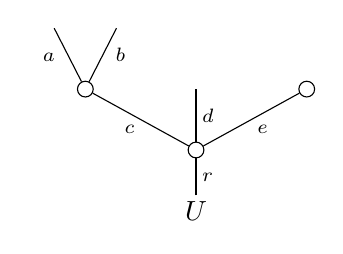
\begin{tikzpicture}[auto,grow=up, level distance = 2.2em,
	every node/.style={font=\scriptsize,inner sep = 2pt}]%
	\tikzstyle{level 2}=[sibling distance=4em]%
	\tikzstyle{level 3}=[sibling distance=2.25em]%
            \node [font=\normalsize] {$U$}
            child{node [dummy] {}
              child{node [dummy] {}
                edge from parent node [swap] {$e$}
              }
              child{edge from parent node [swap] {$d$}}
              child{node [dummy] {}
                child{edge from parent node [near end, swap] {$b$}}
                child{edge from parent node [near end] {$\phantom{b}a$}}
                edge from parent node {$c$}
              }
              edge from parent node [swap] {$r$}
            };        
      \end{tikzpicture}
\end{equation}
Edges with no vertices $\circ$ above them are called \textit{leaves}, the unique bottom edge is called the \textit{root},
and edges that are neither are called \textit{inner edges};
in the example above, $a$ and $b$ are leaves, $r$ is the root, and $c$ and $e$ are inner edges.
The sets of edges, inner edges, leaves, and vertices of a tree $U$ are denoted $\boldsymbol{E}(U)$, $\boldsymbol{E}^{\mathsf{i}}(U)$, and $\boldsymbol{V}(U)$ respectively.
If an edge $t$ is pictorially above (or equal to) an edge $s$, we write $t \leq_d s$.

A map of trees $\varphi \colon U \to V$ is defined to be
a map of edge sets 
$\varphi \colon \boldsymbol{E}(U) \to \boldsymbol{E}(V)$
which preserves
{\color{blue} the broad poset/operadic structure}
(see e.g. \cite[\S 2.1]{BP_edss} for a rigorous definition).

We will also find it convenient to assume that 
each tree $U \in \Omega$ 
is equipped with a \textit{planar structure}.
Informally, 
this means that each object $U$
has a preferred planar representation as in \eqref{eq:TREE}
(a more formal definition of planar structures as
suitable extensions of the partial order $\leq_d$ to a total order
can be found in \cite[\S 3.1]{BP_geo}).
Moreover, we will then prefer to work with a model of $\Omega$
for which the subcategory of planar maps is skeletal,
i.e. such that the only planar isomorphisms are the identities.




\begin{notation}
      We write $\eta$ for the \textit{stick} tree, the unique tree with a single edge and no vertices.
\end{notation}











\begin{example}
      \label{TREEMAP_EX}
      The labels on the edges of the tree diagrams below indicate a map to $\boldsymbol{E}(U)$ with $U$ defined as in \eqref{eq:TREE}.
      The maps determined by four leftmost trees are maps of trees, while the rightmost is not.
      \begin{equation}
            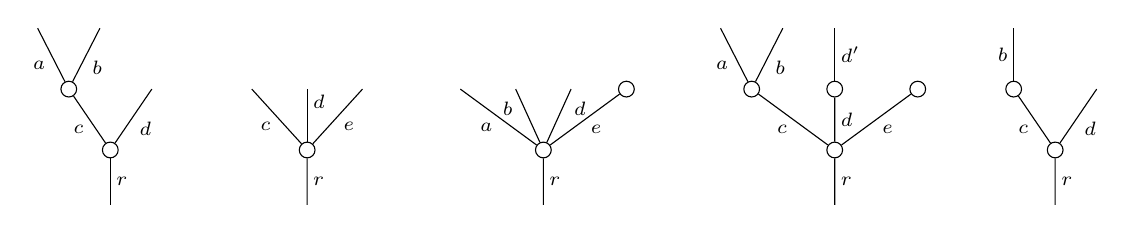
\begin{tikzpicture}[auto, grow=up, level distance = 2.2em,
                  every node/.style={font=\scriptsize,inner sep = 2pt}]
                  \tikzstyle{level 2}=[sibling distance=3em]%
                  \tikzstyle{level 3}=[sibling distance=2.25em]%
                  \node at (0,0) {} % {$T \setminus \set{e}$}
                  child{node [dummy] {}
                    child{edge from parent node [swap] {$d$}}
                    child{node [dummy] {}
                      child{edge from parent node [swap] {$b$}}
                      child{edge from parent node {$a$}}
                      edge from parent node {$c$}
                    }
                    edge from parent node [swap] {$r$}
                  };
                  \tikzstyle{level 2}=[sibling distance=2em]%
                  \node at (2.5,0) {} % {$\partial_{u,v}T$}
                  child{node [dummy] {}
                    child{edge from parent node [swap] {$e$}}
                    child{edge from parent node [swap,near end] {$d$}}
                    child{edge from parent node {$c$}}
                    edge from parent node [swap] {$r$}
                  };
                  \node at (5.5,0) {} % {$\partial_v(T \setminus \set{c})$}
                  child{node [dummy] {}
                    child{node [dummy] {}
                      edge from parent node [swap] {$e$}
                    }
                    child{edge from parent node [swap, very near end] {$d$}}
                    child{edge from parent node [very near end] {$b$}}
                    child{edge from parent node {$a$}}
                    edge from parent node [swap] {$r$}
                  };
                  \tikzstyle{level 2}=[sibling distance=3em]%
                  \node at (9.2,0) {} % {$\sigma_d T$}
                  child{node [dummy] {}
                    child{node [dummy] {}
                      edge from parent node [swap] {$e$}
                    }
                    child{node [dummy] {}
                      child{edge from parent node [swap] {$d'$}}
                      edge from parent node [swap] {$d$}
                    }
                    child{node [dummy] {}
                      child{edge from parent node [swap] {$b$}}
                      child{edge from parent node {$a$}}
                      edge from parent node {$c$}
                    }
                    edge from parent node [swap] {$r$}
                  };                    
                  \node at (12,0) {}
                  child{node [dummy] {}
                    child{edge from parent node [swap] {$d$}}
                    child{node [dummy] {}
                      child{edge from parent node {$b$}}
                      edge from parent node {$c$}
                    }
                    edge from parent node [swap] {$r$}
                  };
            \end{tikzpicture}
      \end{equation}
\end{example}


A map of trees $\varphi \colon U \to V$ is called:
\begin{itemize}
\item a \textit{tall map} if
      $\varphi(\underline{l}_U) = \underline{l}_V$ and $\varphi(r_U) = r_V$,
      with $\underline{l}_{(-)}$ and $r_{(-)}$ denoting the tuple of leaf edges and the root edge;
\item a \textit{face map} if it is injective on edges;
      an \textit{inner face} if it is also tall, and
      an \textit{outer face} if it does not factor through a non-isomorphism inner face map;
\item a \textit{degeneracy} if is surjective on edges and preserves leaves
      (and is hence tall).
\end{itemize}

Pictorially, an inner face map 
$U\to V$ removes some edges in $V$
(while merging the vertices adjacent to those edges),
outer face maps remove some vertices of $V$ (necessarily outer vertices to ensure the tree remains connected),
and degeneracies collapse some of the unary vertices of $U$.


\begin{example}
      In Example \ref{TREEMAP_EX},
      the first map is an inner face, the second an outer face, the third is a general face, while the fourth is a degeneracy.
\end{example}


\begin{proposition}\label{TREEFACT_PROP}
	[{\cite[Prop. 2.2]{BP_edss}}]
	A map of trees $\varphi \colon U \to V$ has a factorization, unique up to unique isomorphisms,
\begin{equation}\label{TREEFACT_EQ}
	U \xrightarrow{\varphi^-} 
	U' \xrightarrow{\varphi^i} 
	U'' \xrightarrow{\varphi^o} V
\end{equation}
	as a degeneracy followed by an inner face map followed by an outer face map.
\end{proposition}


\begin{remark}\label{TODF REM}
	A map $\psi \colon U \to V$
	is tall (resp. a face)
	iff in the decomposition \eqref{TREEFACT_EQ}
	the component $\psi^o$ (resp. $\psi^-$)
	is an isomorphism.
	As such, by combining the 
	first two (resp. last two)
	maps in \eqref{TREEFACT_EQ}
	one recovers the 
	``tall-outer face'' 
	(resp. ``degeneracy-face'')
	factorization of the map $\varphi$.
\end{remark}


\begin{remark}\label{CNVXM REM}
	Following the previous remark, 
	it is natural to consider the class of maps
	$\psi \colon U \to V$ such that
	the factor $\psi^i$ in \eqref{TREEFACT_EQ}
	is an isomorphism.
	Equivalently, $\psi$ is convex precisely if
	the ``tall-outer face'' and ``degeneracy-face''
	factorizations coincide.
	
	We call these maps \textit{convex},
	since the are readily seen to be 
	characterized by the following property:
	if $e <_d e' <_d e''$
	in $V$ and $e,e''$ are in the image of $\psi$
	then so is $e'$.
	
	Notably, it follows from this characterization that convex maps are closed under composition.
\end{remark}


When accounting for planar structures,
one has the following refinement of \eqref{TREEFACT_EQ}.

\begin{proposition}
      A map of trees $\varphi \colon U \to V$ has a strictly unique factorization
      \begin{equation}
            \label{OMEGAFACT_EQ}
            U \xrightarrow{\varphi^{\simeq}} U_p \xrightarrow{\varphi^-} U' \xrightarrow{\varphi^i} U'' \xrightarrow{\varphi^o} V            
      \end{equation}
      as, in order, an isomorphism followed by
      a planar degeneracy, a planar inner face, and a planar outer face.
\end{proposition}


\begin{remark}
	Generalizing Remarks \ref{TODF REM} and \ref{CNVXM REM},
	one has that for any subset 
	of the symbols $\{\simeq,-,i,o\}$
	in \eqref{OMEGAFACT_EQ},
	the type of maps such that 
	the corresponding factors are identities 
	is closed under composition.
	
	For example, the maps $\psi$ such that 
	$\psi^{\simeq},\psi^{i}$
	are identities are the planar convex maps
	while those maps such that
	$\varphi^{-},\varphi^o$
	are identities are the (not necessarily planar) inner face maps,
	both of which are closed under composition.	
\end{remark}



\begin{remark}
      The subcategory of corollas and isomorphisms is isomorphic to the category $\Sigma$ of standard finite ordered sets and (non-ordered) isomorphisms.
\end{remark}


\begin{notation}
      \label{LR_NOT}
      For each $U \in \Omega$, there exists a unique corolla $\mathsf{lr}(U) \in \Sigma$ equipped with a planar tall map $\mathsf{lr}(U) \to U$,
      which we call the \textit{leaf-root} of $U$.
\end{notation}



Next, we consider categories of (colored) forests (cf. \cite[Defn. 2.56]{BP_HGOP}).

\begin{definition}
      The category $\Phi$ of \textit{forests} is the coproduct completion of the category $\Omega$ of trees:
      objects are formal coproducts 
      $F = \amalg_{i \in I} F_i$ with $F_i \in \Omega$,
      and an arrow 
      $\varphi \colon \amalg_{i \in I} F_i \to
      \amalg_{j \in J} F'_j$ is given by
      a map $\varphi \colon I \to J$ and
      maps $\varphi_i \colon F_i \to F'_{\varphi(i)}$ in $\Omega$ for each $i \in I$.

The sets of \emph{edges}, \emph{inner edges}, \emph{vertices}
of a forest $F = \amalg_i F_i$
are defined in the obvious way as
\[
	\boldsymbol{E}(F)
	\simeq
	\amalg_i \boldsymbol{E}(F_i),
\qquad
	\boldsymbol{E}^{\mathsf{i}}(F)
	\simeq
	\amalg_i \boldsymbol{E}^{\mathsf{i}}(F_i),
\qquad
	\boldsymbol{V}(F)
	\simeq
	\amalg_i \boldsymbol{V}(F_i).
\]
\end{definition}


\begin{definition}\label{CFOREST_DEF}
      Let $\mathfrak C$ be a set of colors.
      The category $\Phi_{\mathfrak C}$ of \textit{$\mathfrak C$-forests} has
      \begin{itemize}
      \item objects pairs $\vect F = (F, \mathfrak c)$ with
            $F \in \Phi$ a forest and
            $\mathfrak c \colon \boldsymbol{E}(F) \to \mathfrak C$ a coloring of its edges.
      \item arrows $\vect F = (F, \mathfrak c) \to (F', \mathfrak c') = \vect{F'}$ maps
            $\varphi \colon F \to F'$ in $\Phi$ such that $\mathfrak c = \mathfrak c' \varphi$.
      \end{itemize}      

      These naturally assemble into a category $\Phi_\bullet \to \Set$ fibered over $\Set$.
      Moreover, we denote by
      $\Phi_\bullet^0 \subseteq \Phi_\bullet$
      the wide subcategory of those arrows whose maps on uncolored forests are outer faces.
      
      Moreover, we write
      $\Omega_{\mathfrak{C}} \subset \Phi_{\mathfrak{C}}$,
      which we call the category of 
      \emph{$\mathfrak{C}$-trees},
      for the full subcategory spanned by the objects 
      whose underlying forest is a tree,
      and 
      $\Sigma_{\mathfrak{C}} \subset \Omega_{\mathfrak{C}}$,
      which we call the category of 
      \emph{$\mathfrak{C}$-corollas},
      for the further subcategory of objects whose underlying tree is a corolla
      and whose maps are isomorphisms.
\end{definition}




\subsection{The category of equivariant trees}
\label{GTREES SEC}

We now recall the category $\Omega_G$ of equivariant trees, which encodes the combinatorics of compositions of norm maps;
a thorough discussion can be found in \cite{Per18} or \cite[\S 2]{BP_edss}.

We begin with an explicit example.
Let $G = D_{4} = \set{1,\rho,\rho^2,\rho^3, \sigma, \rho\sigma, \rho^2\sigma, \rho^3\sigma}$
be the dihedral group with 8 elements,
and $L \leq K \leq H \leq G$ denote the subgroups
$H = \langle \rho^2,\sigma \rangle$, $K = \langle \rho^2 \rangle$, $L = \{1\}$.
Then we have a $G$-tree $T$ as below,
with the \textit{expanded representation} given by the two trees on the left below,
and the \textit{orbital representation} given by the single decorated tree on the right.
\begin{equation}
      \label{GTREE_EQ}
      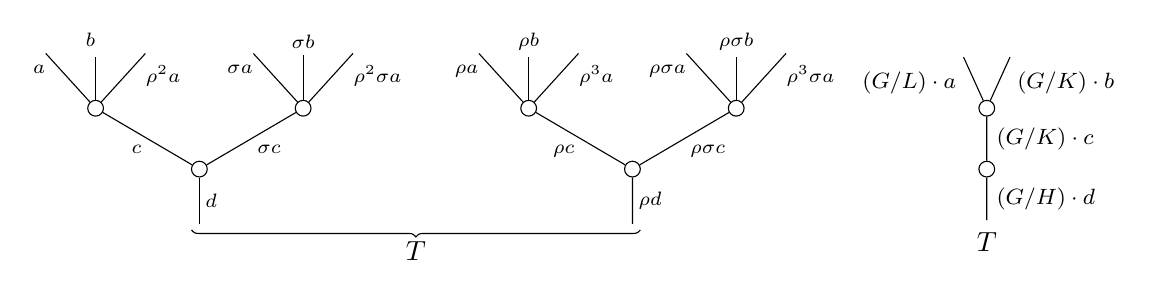
\begin{tikzpicture}[auto,grow=up, level distance = 2.2em,
            every node/.style={font=\scriptsize,inner sep = 2pt}]%
            \tikzstyle{level 2}=[sibling distance=7.5em]%
            \tikzstyle{level 3}=[sibling distance=2em]%
            \node at (5.5,0){}%	
            child{node [dummy] {}%
              child{node [dummy] {}%
                child{node {}%
                  edge from parent node [swap,very near end] {$\rho^3 \sigma a$}}%
                child[level distance = 2.4em]{node {$\rho\sigma b$}}%
                  % edge from parent node [swap,near end] {$\rho\sigma b$}}%
                child{node {}%
                  edge from parent node [very near end] {$\rho \sigma a$}}%
                edge from parent node [swap] {$\rho \sigma c$}}%
              child{node [dummy] {}%
                child{node {}%
                  edge from parent node [swap,very near end] {$\rho^3 a$}}%
                child[level distance = 2.4em]{node {$\rho b$}}%
                % edge from parent node [swap,near end] {$\rho b$}}%
                child{node {}%
                  edge from parent node [very near end] {$\rho a$}}%
                edge from parent node  {$\rho c$}}%
              edge from parent node [swap] {$\rho d$}};%
            \node at (0,0){}%	
            child{node [dummy] {}%
              child{node [dummy] {}%
                child{node {}%
                  edge from parent node [swap,very near end] {$\rho^2\sigma a$}}%
                child[level distance = 2.4em]{node {$\sigma b$}}%
                % edge from parent node [swap,near end] {$\sigma b$}}%
                child{node {}%
                  edge from parent node [very near end] {$\sigma a$}}%
                edge from parent node [swap] {$\sigma c$}}%
              child{node [dummy] {}%
                child{node {}%
                  edge from parent node [swap,very near end] {$\rho^2 a$}}%
                child[level distance = 2.4em]{node {$b\phantom{j}$}}%
                % edge from parent node [swap,near end] {$b\phantom{j}$}}%
                child{node {}%
                  edge from parent node [very near end] {$a$}}%
                edge from parent node  {$c$}}%
              edge from parent node [swap] {$d$}};%
            \begin{scope}[every node/.style={font=\footnotesize}]%
                  \node at (10,0) {}
                  child{node [dummy] {}%
                    child{node [dummy] {}%
                      child{node {}%
                        edge from parent node [swap,very near end] {$(G/K) \cdot b$}}%
                      child{node {}%
                        edge from parent node [very near end] {$(G/L) \cdot a$}}%
                      edge from parent node [right] {$(G/K) \cdot c$}}%
                    edge from parent node [right] {$(G/H) \cdot d$}};%
            \end{scope}%
            \draw[decorate,decoration={brace,amplitude=2.5pt}] (5.6,0) -- (-0.1,0) node[midway,inner sep=4pt,font=\normalsize]{$T$}; %
            \node at (10,-0.15) [font=\normalsize] {$T$}; 
     \end{tikzpicture}%
\end{equation}
The expanded representation is a planar representation of the $G$-sets of edges and vertices, equipped with names for the edges which indicate the group action on the set of edges (and hence also vertices).
In the orbital representation, each edge indicates an orbit worth of edges from the expanded representation,
and is labeled by the appropriate transitive $G$-set.

In general, we have the following.
\begin{definition}
      Let $\Phi^G$ denote the category of forests with $G$-action. 
      The category $\Omega_G$ of \textit{$G$-trees} is the full subcategory of $\Phi^G$ spanned by those $G$-forests whose
      $G$-set $I$ of tree components has a transitive $G$-action.
\end{definition}

\begin{remark}
      We can describe $G$-trees in $\Omega_G$ by
      $T = \amalg_{i \in I} T_i$ with $I$ a transitive $G$-set and $T_i$ trees.
      Alternatively, any choice of component $T_{\**}$ has a stabilizer $H \leq G$, and then we have a decomposition
      $T \simeq G \cdot_H T_{\**}$.
      Finally, if $\Gamma \leq G \times \Aut(T_{\**})$ is the {\color{blue}graph subgroup} \todo{graph subgroup hasn't been defined yet} encoding the $H$-action on $T_{\**}$, we have
      $T \simeq G \cdot T_{\**}/\Gamma$.
\end{remark}

For $T \in \Omega_G$, we write
$\boldsymbol{E}_G(T) = \boldsymbol{E}(T)/G$, $\boldsymbol{E}^i_G(T) = \boldsymbol{E}^i(T)/G$, $\boldsymbol{V}_G(T) = \boldsymbol{V}(T)/G$
for the set of \textit{edge orbits}, \textit{inner edge orbits}, and \textit{$G$-vertices}, respectively.

\begin{remark}
      $\Omega_G$ is fibered over the \textit{orbit category} $\mathsf O_G$ of transitive $G$-sets and $G$-maps,
      by the functor which sends a $G$-tree $T = \amalg_{i \in I} T_i$ to its $G$-set of tree components $I$.
\end{remark}


\begin{remark}
      The two representations of $G$-trees from \eqref{GTREE_EQ} play complementary roles in our analysis:
      the expanded representation displays all of the relevant edge information, and thus is often useful for describing maps between $G$-trees;
      conversely, the orbital representation compactly displays the relevant data for composing norm maps of operads (e.g. {\color{blue} Example \ref{GTREENORM_EX}}).
\end{remark}

As in $\Omega$,
maps $\varphi \colon S \to T$ between $G$-trees
can be built from a few basic types of maps.
In each fiber over $\mathsf O_G$ 
(i.e. if $\varphi$ is an identity between tree components), we say $\varphi$ is an
\textit{(inner, outer) face map}, \textit{degeneracy map}, \textit{tall map}, or \textit{planar map} if
$\varphi_j \colon S_j \to T_{\varphi(j)}$ is so for some (and thus all) $j \in J$.
The cartesian arrows are a new type of map, dubbed \textit{quotients},
which act as twisted fold maps on the forest components;
explicitly, $\varphi$ is a quotient iff $\varphi_j \colon S_j \to T_{\varphi(j)}$ is an isomorphism for some (and thus all) $j \in J$.

We give a minimal example of a quotient below. 
Further discussion and examples can be found in \cite[Rem. 5.49]{Per18}.
\begin{example}
      Let $G = \mathbb Z/ 2\mathbb Z$ be the cyclic group with two elements.
      We have the following quotient map on $G$-corollas,
      where $\alpha \mapsto a$, $\alpha^- \mapsto -a$, $\beta \mapsto b$, $\gamma \mapsto c$.
      \[
            \begin{tikzpicture}[grow=up,auto,level distance=2.4em,
                  every node/.style={font=\scriptsize,inner sep = 2pt}]%
                  \tikzstyle{level 2}=[sibling distance=4em]%
                  \begin{scope}[every node/.style={font=\footnotesize}]%
                        \node at (0,0) {}
                        child{node [dummy] {}
                          child{edge from parent node [swap,near end] {$G/e+\alpha^{-}$}}
                          child{node {$G/e + \beta$}}
                          child{edge from parent node [near end] {$G/e + \alpha$}}
                          edge from parent node [swap] {$G/2 + \gamma$}
                        };
                        % 
                        \node at (4.8,1) {$\xrightarrow{\qquad \qquad}$};
                        % 
                        \node at (8,0) {}
                        child{node [dummy] {}
                          child{edge from parent node [swap] {$G/G + b$}}
                          child{edge from parent node {$G/e+a$}}
                          edge from parent node [swap] {$G/G+c$}
                        };
                  \end{scope}%
                  \begin{scope}[level distance=2em]
                        \tikzstyle{level 2}=[sibling distance=3em]%
                        \node at (-2,-2.5) {}
                        child{node [dummy] {}
                          child{edge from parent node [swap, near end] {$\alpha^{-}$}}
                          child{edge from parent node [swap, very near end] {$\beta$}}
                          child{edge from parent node [near end] {$\alpha$}}
                          edge from parent node [swap] {$\gamma$}
                        };
                        \node at (2,-2.5) {}
                        child{node [dummy] {}
                          child{edge from parent node [swap, near end] {$-\alpha^{-}$}}
                          child{edge from parent node [swap, very near end] {$-\beta$}}
                          child{edge from parent node [near end] {$-\alpha$}}
                          edge from parent node [swap] {$-\gamma$}
                        };
                        \node at (4.8,-1.7) {$\xrightarrow{ \qquad \qquad}$};
                        \node at (8,-2.5) {}
                        child{node [dummy] {}
                          child{edge from parent node [swap, near end] {$-a$}}
                          child{edge from parent node [swap, very near end] {$b$}}
                          child{edge from parent node [near end] {$a$}}
                          edge from parent node [swap] {$c$}
                        };                  
                  \end{scope}
                  \draw[decorate,decoration={brace,amplitude=2.5pt}] (2.1,-2.5) -- (-2.1,-2.5) node[midway,inner sep=4pt,font=\normalsize]{$S$}; %
                  \node at (8,-2.65) [font=\normalsize] {$T$};
                  \node at (8,-.15) [font=\normalsize] {$T$};
                  \node at (0,-.15) [font=\normalsize] {$S$};
            \end{tikzpicture}
      \]
\end{example}

\begin{corollary}[{cf. \cite[Rem. 5.49]{Per18}}]
	A map $\phi \colon S \to T$ in $\Omega_G$ has a factorization, unique up to unique isomorphisms,
\[
	S \xrightarrow{\phi^-} 
	S' \xrightarrow{\phi^i} 
	S'' \xrightarrow{\phi^o} 
	q^{\**}T \xrightarrow{q} T
\]
	as, in order: a degeneracy map $\phi^-$, an inner face map $\phi^i$, an outer face map $\phi^o$, and a quotient map $q$.
\end{corollary}

\begin{definition}
      We denote by $\Omega_G^0 \subseteq \Omega_G$ the wide subcategory of $G$-trees and quotient maps.
      Further, we write $\Sigma_G \subseteq \Omega_G^0$ for the full subcategory spanned by \textit{$G$-corollas} and quotient maps,
      where $C \in \Omega_G$ is a $G$-corolla if $|\boldsymbol{V}_G(C)| = 1$.
\end{definition}
      
\begin{notation}
      \label{LRG_NOT}
      As in Notation \ref{LR_NOT}, 
      for any $T = \amalg_{i \in T}T_i \in \Omega_G$ there exists a unique $G$-corolla $\mathsf{lr}(T) \in \Sigma_G$ equipped with a planar tall map $\mathsf{lr}(T) \to T$
      called the \textit{leaf-root} of $T$.
      Explicitly, $\mathsf{lr}(T) = \amalg_{i \in I} \mathsf{lr}(T_i)$.
\end{notation}


Finally, contrasting with the above, we define the faces of a $G$-trees non-equivariantly.

\begin{definition}
	Let $T = \amalg_i T_i \in \Omega_G$ be a $G$-tree.
	An \textit{(outer) face} of $T$ is an (outer) face map $U \to T_i$ from some $U \in \Omega$ to a component $T_i$ of $T$.
	A face of $T$ is called \textit{planar} if the map $U \to T_i$ preserves the planar order.

	Let $\mathsf{Face}(T)$ denote the $G$-poset of planar faces of $T$,
	and let $\mathsf{Face}_{\mathsf{sc}}(T) \subseteq \mathsf{Face}(T)$ denote the subposet spanned by the planar outer faces of $T$ with no inner edges.
\end{definition}





\subsection{Equivariant dendroidal sets}
\label{EDS_SEC}

As {\color{red} discussed in the introduction},
recall that the category of 
\emph{dendroidal sets}
is the presheaf category
$\mathsf{dSet} = \mathsf{Set}^{\Omega^{op}}$.
Further for a (finite) group $G$,
the category of
\emph{$G$-equivariant dendroidal sets}
is then the $G$-object category
$\mathsf{dSet}^G = \mathsf{Set}^{G \times \Omega^{op}}$.


One key subtlety when working with 
$\mathsf{dSet}^G$
is that for each equivariant dendroidal set 
$X \in \mathsf{dSet}^G$
its levels $X(U)$ are indexed by
non-equivariant trees $U \in \Omega$,
while the key classes of maps in $\mathsf{dSet}^G$ are defined in terms
of $G$-trees $T \in \Omega_G$.

To make this precise, 
we first extend the Yoneda embedding
$\Omega[-]\colon \Omega \to \mathsf{dSet}$
notation
for the representable functors
$\Omega[U](V) = \Omega(V,U)$
to obtain extended Yoneda embeddings
(here the right embedding is simply obtained from the left embedding by taking $G$-objects)
\begin{equation}\label{FORESREP EQ}
\begin{tikzcd}[row sep=0]
	\Phi \ar{r}{\Omega[-]}
&
	\mathsf{dSet}
&&%%
	\Phi^G \ar{r}{\Omega[-]}
&
	\mathsf{dSet}^G
\\
	\amalg_i F_i
	\ar[mapsto]{r}
&
	\amalg_i \Omega[F_i]
&&%%
	\amalg_i F_i
	\ar[mapsto]{r}
&
	\amalg_i \Omega[F_i]
\end{tikzcd}
\end{equation}
Next, note that since $G$-trees $\Omega_G$
are defined as a subcategory of $G$-forests $\Phi^G$,
the right side of 
\eqref{FORESREP EQ}
defines representables 
$\Omega[T] \in \mathsf{dSet}^G$
for $T \in \Omega_G$.
These representable presheaves 
$\Omega[T]$
are then the basis for
generalizing several fundamental
presheaves in dendroidal sets $\mathsf{dSet}$
{\color{red} add some Moerdijk reference}
to equivariant dendroidal sets
$\mathsf{dSet}^G$
(cf. \cite[\S 6]{Per18}),
as follows.



\begin{definition}\label{DSETPRESHEAF_DEF}
	For $T = \amalg_i T_i$ a $G$-tree,
	we define the \emph{boundary}
	$\partial \Omega[T] \subseteq \Omega[T]$ by
\begin{equation}
	\partial \Omega[T] = 
	\amalg_i \partial \Omega[T_i]
	= \mathop{\colim}\limits_{U \in \mathsf{Face}(T), U \neq T} \Omega[U]
	= \bigcup_{U \in \mathsf{Face}(T), U \neq T} \Omega[U].
\end{equation}
	Next, for $\emptyset \neq E \subseteq \boldsymbol{E}^{\mathsf{i}}(T)$ a non-empty $G$-subset of inner edges, we write $E_i = E \cap \boldsymbol{E}(T_i)$
	and define the associated \textit{$G$-inner horn} by
\begin{equation}\label{GINNERHORN_EQ}
	\Lambda^{E}[T] = \amalg_i \Lambda^{E_i}[T_i]
	= \mathop{\colim}\limits_{U \in \mathsf{Face}(T), (T_i - E_i) \not\into U} \Omega[U]
	= \bigcup_{U \in \mathsf{Face}(T), (T_i - E_i) \not\into U} \Omega[U].
\end{equation}
	Finally, the \textit{Segal core} of $T$ is
\begin{equation}\label{eq:SC}
	Sc[T] = 
	\amalg_i Sc[T_i] =
	\mathop{\colim}\limits_{U \in \mathsf{Face}_{\mathsf{sc}}(T)} \Omega[U] =
	\bigcup_{U \in \mathsf{Face}_{\mathsf{sc}}(T)} \Omega[U].
\end{equation}
\end{definition}


\begin{remark}
For $T \in \Omega_G$, a decomposition $T \simeq G \cdot_H T_{\**}$ with $T_{\**} \in \Omega^H$ yields
\[
	\Omega[T] \simeq G \cdot_H \Omega[T_{\**}],
\qquad
	\partial\Omega[T] \simeq G \cdot_H \partial \Omega[T_{\**}],
\qquad
	\Lambda^{E}[T] \simeq G \cdot_H \Lambda^{E_{\**}}[T_{\**}],
\qquad
	Sc[T] \simeq G \cdot_H Sc[T_{\**}].
\]
      % where $E_{\**} = E \cap \boldsymbol{E}(T_{\**})$.
\end{remark}


Mimicking the non-equivariant story, the maps in Definition \ref{DSETPRESHEAF_DEF} are then the basis for a model structure on $\dSet^G$.

In the following, we recall that a class of maps is called \textit{saturated} if it is closed under pushouts, retracts, and transfinite compositions.

\begin{definition}
	The class of \textit{$G$-normal monomorphisms}
	in $\mathsf{dSet}^G$
	is the saturation of the boundary inclusions 
	$\partial \Omega[T] \into \Omega[T]$ for $T \in \Omega_G$.
	
	The class of \textit{$G$-inner anodyne extensions}
	in $\mathsf{dSet}^G$
	is the saturation of the $G$-inner horn inclusions
	$\Lambda^E [T] \into \Omega[T]$ 
	for $T \in \Omega_G$ and $G$-subset
	$\emptyset \neq E \subseteq
	\boldsymbol{E}^{\mathsf{i}}(T).$
\end{definition}



\begin{definition}
	A map $X \to Y$ in $\dSet^G$
	is called a \emph{$G$-inner fibration}
	if it has the right lifting property
	with respect to all $G$-inner horn inclusions
	$\Lambda^E[T] \to \Omega[T]$.
	
	Moreover, 
	if $X \to \**$
	is a $G$-inner fibration
	then 
	$X \in \dSet^G$ is called a \textit{$G$-$\infty$-operad}.
\end{definition}


Informally,
$G$-$\infty$-operads can be thought of as
``operads with weak composition laws for norm maps''.


%\begin{example}
%       We recall the setup of \eqref{GTREE_EQ}, with $G = D_8$, $H = \langle \sigma^2,\rho \rangle$, $K = \langle \sigma^2 \rangle$, $L = \**$, and $T$ the given tree diagram.
%       Let $X \in \dSet^G$. Then we have natural solid arrows
%       \[
%             \begin{tikzcd}
%                   X(H/K) \times X(K/L \amalg K/K) \arrow[r, start anchor = east, end anchor = west, dashed, bend left, shift left]
%                   &
%                   \Hom_{\dSet^G}(\Omega[T], X) \arrow[l, shift left] \arrow[r]
%                   &
%                   X(H/L \amalg H/K)
%             \end{tikzcd}
%      \]
%       given by the presheaf structure,
%       If $X$ is a $G$-$\infty$-operad, there exists a dashed section (possibly many) as written,
%       and the composite map provides a choice of a composition law.
%       providing a choice of composition.     
%\end{example}



To recall the model structure on $\mathsf{dSet}^G$,
we need two more ingredients.
First, we write
\begin{equation}\label{IOTASHADJ EQ}
	\iota_! \colon 
	\mathsf{sSet}
	\rightleftarrows
	\mathsf{dSet}
	\colon
	\iota^{\**}
\qquad
	\iota_! \colon 
	\mathsf{Cat}
	\rightleftarrows
	\mathsf{Op}
	\colon
	\iota^{\**}
\end{equation}
for the adjunctions
where the left adjoints $\iota_!$
are the natural inclusions.
Note that the left adjunction is induced by the natural inclusion
$\iota \colon \Delta \to \Omega$.
Second, we write
\begin{equation}\label{TAUADJ EQ}
	\tau \colon 
	\mathsf{sSet}
	\rightleftarrows
	\mathsf{Cat}
	\colon
	N
\qquad
	\tau \colon 
	\mathsf{dSet}
	\rightleftarrows
	\mathsf{Op}
	\colon
	N
\end{equation}
for the adjunctions where the right adjoints are the 
\emph{nerve functors}
described by
$(N \mathcal{C})(n) = 
\mathsf{Cat}\left([n],\mathcal{C}\right)$
for $\mathcal{C}\in \mathsf{Cat}$
and
$(N \mathcal{O})(T) = 
\mathsf{Op}\left(\Omega(T),\mathcal{O}\right)$
for $\mathcal{O}\in \mathsf{Op}$.
Recall \cite[Prop. 5.3 and Thm. 6.1]{MW09}
that the nerve functors $N$ are fully faithful, 
with their essential image characterized
as those presheaves 
that satisfy a Segal condition.



\begin{theorem}\label{DSETGMOD THM}
	{\cite[Thm 2.1]{Per18}}
There exists a left proper (cf. \cite[Prop. 8.8]{Per18}) model structure on $\dSet^G$ such that:
\begin{itemize}
	\item the cofibrations are the $G$-normal monomorphisms;
	\item the fibrant objects are the $G$-$\infty$-operads;
	\item the fibrations between
	$G$-$\infty$-operads 
	are the $G$-inner fibrations $X \to Y$
	such the induced maps on 
	fixed-point homotopy categories 
	$\tau \iota^{\**}(X^H \to Y^H)$ are isofibrations of categories for all $H \leq G$;
	\item the weak equivalences are the smallest class of maps closed under 2-out-of-3 which
	contains the $G$-inner anodyne extensions and the trivial fibrations
	(i.e. those maps with the right lifting property against the $G$-normal monomorphisms).
\end{itemize}
\end{theorem}

In addition to the category
$\mathsf{dSet}^G = \mathsf{Set}^{G \times \Omega^{op}}$
of equivariant dendroidal sets,
there is also a category
$\mathsf{dSet}_G = \mathsf{Set}^{\Omega_G^{op}}$,
which we call the category of 
\emph{genuine dendroidal sets}.
As it turns out,
some natural constructions in the non-equivariant setting 
generalize to produce objects in 
$\mathsf{dSet}_G$
rather than in 
$\mathsf{dSet}^G$
(e.g. $\mathsf{dSet}_G$ is essential to establishing the characterization
of the fibrant objects in $\mathsf{dSet}^G$,
cf. \cite[\S 8.2]{Per18}),
so we next recall the connection between the two categories.

Let $\mathsf{O}_G$
denote the \emph{orbital category},
i.e. the category of transitive $G$-sets $G/H$ for $H\leq G$ and $G$-set maps.
Regarding the group $G$ as a single object category,
one then has a fully faithful inclusion
$\iota \colon G^{op} \to \mathsf{O}_G$
sending the object of $G$ to the free $G$-set $G/e$. 
In addition, there is a fully faithful inclusion
$\Omega \times \mathsf{O}_G \to \Omega_G$
given by
$(T,G/H) \mapsto G/H \cdot T$.
Altogether, one obtains a commutative diagram of fully faithful inclusions as follows.
\begin{equation}
\begin{tikzcd}[row sep=9,column sep=11]
	&
	\Delta \times \mathsf{O}_G 
	\ar{rd}{\iota}
	\ar[bend left=10]{rrd}{\iota_G}
	&
\\
	\Delta \times G^{op} 
	\ar{ru}{\upsilon}
	\ar{rd}[swap]{\iota}
	&&
	\Omega \times \mathsf{O}_G
	\ar{r}
	&
	\Omega_G
\\
	&
	\Omega \times G^{op}
	\ar{ru}[swap]{\upsilon}
	\ar[bend right=10]{rru}[swap]{\upsilon_G}
	&
\end{tikzcd}
\end{equation}
The connection between 
$\mathsf{dSet}^G$ and $\mathsf{dSet}_G$
is then given by the right adjunction
\begin{equation}\label{UPSILONADJ EQ}
	\upsilon^{\**} \colon 
	\mathsf{sSet}^G
	\rightleftarrows
	\mathsf{sSet}^{\mathsf{O}_G^{op}}
	\colon
	\upsilon_{\**}
\qquad
	\upsilon_G^{\**} \colon 
	\mathsf{dSet}^G
	\rightleftarrows
	\mathsf{dSet}_G
	\colon
	\upsilon_{G,\**}
\end{equation}
where we note that the right adjoints 
$\upsilon_{\**}$, $\upsilon_{G,\**}$
are fully faithful inclusions.

The fully faithful functors appearing in 
\eqref{IOTASHADJ EQ},
\eqref{TAUADJ EQ},
\eqref{UPSILONADJ EQ}
then fit into commutative diagrams
as below where $\mathsf{Op}_G$
is the category of \emph{genuine equivariant operads}.
These are an extension of the notion of operad
which in the single colored context were 
first defined in \cite{BP_geo}
via algebraic means. 
However, to sidestep the technical work needed to extend 
the definition in \cite{BP_geo} 
to the colored context,
here we regard $\mathsf{Op}_G$
simply as the full subcategory of 
$\mathsf{dSet}_G$
of those objects satisfying a Segal condition,
so that the fact that
$N_G$ is fully faithful is tautological.
\begin{equation}\label{ALLFULL EQ}
\begin{tikzcd}
	\mathsf{Cat}^G
	\ar{r}{\iota_!}
	\ar{d}[swap]{N}
	&
	\mathsf{Op}^G
	\ar{r}{\upsilon_{G,\**}}
	\ar{d}[swap]{N}
	&
	\mathsf{Op}_G
	\ar{d}{N_G}
&&
	\mathsf{Cat}^G
	\ar{r}{\upsilon_{\**}}
	\ar{d}[swap]{N}
	&
	\mathsf{Cat}^{\mathsf{O}_G^{op}}
	\ar{r}{\iota_{G,!}}
	\ar{d}[swap]{N}
	&
	\mathsf{Op}_G
	\ar{d}{N_G}
\\
	\mathsf{sSet}^G
	\ar{r}[swap]{\iota_!}
	&
	\mathsf{dSet}^G
	\ar{r}[swap]{\upsilon_{G,\**}}
	&
	\mathsf{dSet}_G
	&&
	\mathsf{sSet}^G
	\ar{r}[swap]{\upsilon_{\**}}
	&
	\mathsf{sSet}^{\mathsf{O}_G^{op}}
	\ar{r}[swap]{\iota_{G,!}}
	&
\mathsf{dSet}_G
\end{tikzcd}
\end{equation}
By taking left adjoints of 
the vertical nerve functors above 
we obtain the following diagram
where those squares that include natural transformations
\emph{do not} commute. 
Here the existence of the dashed left adjoint 
$\tau_G$ to $N_G$
requires justification, 
with a full discussion of $\tau_G$
being the objective of Appendix \ref{HGEO AP}.
\begin{equation}\label{TAUFUNCTS EQ}
\begin{tikzcd}
	\mathsf{sSet}^G
	\ar{r}{\iota^{\**}}
	\ar{d}[swap]{\tau}
	&
	\mathsf{dSet}^G
	\ar{r}{\upsilon_{G,\**}}
	\ar{d}[swap]{\tau}
	&
	\mathsf{dSet}_G
	\ar[dashed]{d}{\tau_G}
	\ar[Rightarrow,dashed]{dl}
&&
	\mathsf{sSet}^G
	\ar{r}{\upsilon_{\**}}
	\ar{d}[swap]{\tau}
	&
	\mathsf{sSet}^{\mathsf{O}_G^{op}}
	\ar{r}{\iota^{\**}_G}
	\ar{d}[swap]{\tau}
	\ar[Rightarrow]{dl}
	&
	\mathsf{dSet}_G
	\ar[dashed]{d}{\tau_G}
\\
	\mathsf{Cat}^G
	\ar{r}[swap]{\iota^{\**}}
	&
	\mathsf{Op}^G
	\ar{r}[swap]{\upsilon_{G,\**}}
	&
	\mathsf{Op}_G
&&
	\mathsf{Cat}^G
	\ar{r}[swap]{\upsilon_{\**}}
	&
	\mathsf{Cat}^{\mathsf{O}_G^{op}}
	\ar{r}[swap]{\iota_{G}^{\**}}
	&
	\mathsf{Op}_G
\end{tikzcd}
\end{equation}





\section{The tame model structure on preoperads}
\label{TAME_SEC}


{\color{orange}
  In this section, we build an auxiliary model structure on pre-operads,
  Quillen equivalent to the model structure introduced in \cite{BP_edss} and recalled in \S \ref{SPREOP_SEC} below.
}

First, we review the model structures on
simplicial dendroidal sets $\mathsf{sdSet}^G$
and preoperads $\mathsf{PreOp}^G$ built in \cite{BP_edss}.


\subsection{Equivariant dendroidal Segal spaces}
\label{JT_SEC}


We now recall the several model structures on the category of
\textit{equivariant simplicial dendroidal sets}
$\mathsf{sdSet}^G = \Set^{\Delta^{op} \times \Omega^{op} \times G}$
introduced in \cite{BP_edss}.

We first recall some notation for objects in $\mathsf{sdSet}^G$.

\begin{notation}
      For $X \in \mathsf{sdSet}^G$, we write $X_n(U)$ for the evaluation at $n \in \Delta$ and $U \in \Omega$,
      and refer to $n$ and $U$ as the \textit{simplicial} and \textit{dendroidal} directions.
      More generally, we write
      \begin{equation}
            \label{SDSET_EQ}
            X_{(-)} \colon \sSet \to \dSet^G,
            \qquad
            X(-) \colon \dSet^G \to \sSet
      \end{equation}
      for the colimit-preserving functors
      such that $X_{\Delta[n]} = X_n$ and 
      $X\left(G \cdot\Omega[U]\right) = X(U)$ for $n \geq 0$, $U \in \Omega$.
      Explicitly, $X_K(U) = \sSet(K, X(U))$ and $X(A)_n = \dSet^G(A, X_n)$.
      
	Additionally, we have natural fully-faithful inclusions
	(as presheaves that are constant along one of the directions)
\[
	c_{!} \colon \dSet^G \longto \mathsf{sdSet}^G,
		\qquad
	c'_! \colon \sSet \longto \mathsf{sdSet}^G
\]
	and we will often identify presheaves with their images under $c_!$ or $c'_!$.

	Lastly, for $A \in \dSet^G$ and $K \in \sSet$ we write $A \times K$ for the presheaf $(A \times K)_n(U) = A(U) \times K_n$.
\end{notation}


The various model structures on $\mathsf{sdSet}^G$ arise
from the theory of (generalized) Reedy categories.


First, since $\Delta^{op}$ is a Reedy category,
the identification
$\mathsf{sdSet}^G \simeq 
\left(\mathsf{dSet}^G\right)^{\Delta^{op}}$
together with the model structure on 
$\mathsf{dSet}^G$ from \cite{Per18}
(cf. Theorem \ref{DSETGMOD THM})
yields the 
\textit{simplicial Reedy model structure} on $\mathsf{sdSet}^G$.
Note that the weak equivalences in this model structure
are the \textit{dendroidal equivalences},
i.e. the maps
$f \colon X \to Y$
such that $X_n \to Y_n$ is a weak equivalence in $\dSet^G$ for all $n \geq 0$.

Second, as discussed in 
\cite[Ex. A.7]{BP_edss},
$\Omega^{op} \times G$ is \emph{a generalized Reedy category}
and the family of {\color{blue} graph subgroups} is
\emph{Reedy admissible}
in the sense of \cite[Ex. A.2]{BP_edss}.
Hence, by \cite[Thm. A.8]{BP_edss},
the identification 
$\mathsf{sdSet}^G \simeq 
\mathsf{sSet}^{\Delta^{op} \times G}$
together with the Kan model structure on 
$\mathsf{sSet}$
yields the 
\textit{(equivariant) dendroidal Reedy model structure} on $\mathsf{sdSet}^G$.
The weak equivalences in this model structure are the
\emph{simplicial equivalences},
i.e. the maps $f \colon X \to Y$
such that 
$X(\Omega[T]) \to Y(\Omega[T])$
are Kan equivalences in $\mathsf{sSet}$
for each $T \in \Omega_G$.

Third, as the simplicial and dendroidal Reedy model structures
in $\mathsf{sdSet}^G$ above have the same cofibrations,
the joint left Bousfield localization framework in 
\cite[\S 4.1]{BP_edss}
yields the following.


\begin{theorem}\label{JB_THM}
	The simplicial and dendroidal Reedy model structures on 
	$\mathsf{sdSet}^G$
	have a smallest\footnote{Here ``smallest'' means that the class of weak equivalences is as small as possible.}
	common left Bousfield localization,
	which we call the \emph{joint Bousfield localization}.
	Moreover:
\begin{enumerate}[label = (\roman*)]
	\item \label{PROPER_LBL}
	the joint Bousfield localization is left proper;
	\item \label{SDEQUIV_LBL}
	both the dendroidal and simplicial equivalences in $\mathsf{sdSet}^G$ are also joint equivalences;
	\item \label{JTFIB_LBL}
	$X$ is joint fibrant iff $X$ is both simplicial and dendroidal Reedy fibrant;
	\item \label{SFIB_JEQ_LBL} if $X,Y$ are joint fibrant
	then a map $X \to Y$ is a joint equivalence iff it is a simplicial
	equivalence iff it is a dendroidal equivalence;
	\item \label{DFIB_JEQ_LBL} if $X,Y$ are dendroidal fibrant
	then a map $X \to Y$ is a joint equivalence iff 
	it is a dendroidal equivalence iff $X_0 \to Y_0$ is an equivalence in $\mathsf{dSet}^G$;
	\item \label{JTCFIB_MAP_LBL} 
	if $X \to Y$ is a joint (co)fibration,
	the level maps 
	$X_n \to Y_n, n \geq 0$
	are (co)fibrations in $\mathsf{dSet}^G$
	and the maps
	$X\left(\Omega[T]\right) \to Y\left(\Omega[T]\right), T \in \Omega_G$
	are (co)fibrations in $\mathsf{sSet}$.

	In particular, if 
	$X$ is joint fibrant
	then $X_n \in \dSet^G$ and $X(\Omega[T]) \in \sSet$ are fibrant.
\end{enumerate}
\end{theorem}



\begin{proof}
	The existence of a smallest common left Bousfield localization is 
	an application of \cite[Prop. 4.1]{BP_edss}
	with the hypothesis that the dendroidal/simplicial Reedy model structures admit localizations being guaranteed by 
	Hirchhorn's existence result 
	\cite[Thm. 4.1.1]{Hir03}.
	\ref{PROPER_LBL} then follows from \cite[Thm. 4.1.1(3)]{Hir03}.
	\ref{SDEQUIV_LBL} holds by definition.
	\ref{JTFIB_LBL} and \ref{SFIB_JEQ_LBL} are \cite[Prop. 4.1(i)(ii)]{BP_edss}.
	\ref{DFIB_JEQ_LBL} is \cite[Cor. 4.29(iii)]{BP_edss}.
	Lastly, \ref{JTCFIB_MAP_LBL} follows from \cite[Lemmas A.27(i), A.29(i)]{BP_edss}.
\end{proof}


Fourth (and last), one has the \textit{(equivariant) dendroidal Segal space} model structure on $\mathsf{sdSet}^G$,
which is the localization of the dendroidal Reedy model structure with respect to the Segal core inclusions
\[
	Sc[T] \longto \Omega[T],
\qquad
	T \in \Omega_G.
\]



\begin{lemma}\label{FCOLIM_WE_LEM}
	The weak equivalences in the dendroidal Reedy, dendroidal Segal space, and joint Reedy model structures 
	on $\mathsf{sdSet}^G$ are closed under filtered colimits.
\end{lemma}

\begin{proof}
	Weak equivalences in the dendroidal Reedy model structure are simplicial equivalences, 
	so in that case the result is inherited from the analogous claim for $\mathsf{sSet}$.
%	
	The result for the latter two model structures follows
	since they are left Bousfield localizations of the dendroidal Reedy model structure.
	{\color{red} not exactly obvious: this needs either a proper reference or a further argument}
\end{proof}






\subsection{Segal preoperads}
\label{SPREOP_SEC}


In this section we recall the normal model structure on preoperads
$\mathsf{PreOp}^G$
introduced and studied in \cite[\S 4 and \S 5]{BP_edss}.

\begin{definition}\label{PREOP DEF} 
	The category of \textit{(equivariant) preoperads} $\mathsf{PreOp}^G$ is the full subcategory of $\mathsf{sdSet}^G$ spanned by those $X$ such that
	$X(\eta)$ is a discrete simplicial set.
\end{definition}



\begin{definition}
	Given $X \in \mathsf{PreOp}^G$ we call $X(\eta)$ the 
	\emph{color set of $X$}
	and denote the associated \emph{color set functor} as follows.
	\begin{equation}\label{COLORSET EQ}
	\begin{tikzcd}[row sep=0]
	\mathsf{PreOp}^G \ar{r}{\mathfrak{C}_{\bullet}} &
	\mathsf{Set}^G
	\\
	X \ar[mapsto]{r} &
	\mathfrak{C}_X = X(\eta)
	\end{tikzcd}
	\end{equation}

Further, for each fixed $\mathfrak{C} \in \mathsf{Set}^G$ we write 
$\mathsf{PreOp}^G_{\mathfrak{C}} \subset \mathsf{PreOp}^G$
for the fiber subcategory of 
\eqref{COLORSET EQ}
over $\mathfrak{C}$,
consisting of those $X$
such that $X(\eta) = \mathfrak{C}$
and maps that are the identity on colors.	
	
	
	Lastly, for $f \colon \mathfrak{C} \to \mathfrak{D}$
	be a map of $G$-sets of colors
	we define adjoint functors
	\[
	f_{!} \colon
	\mathsf{PreOp}^{G}_{\mathfrak{C}}
	\rightleftarrows
	\mathsf{PreOp}^{G}_{\mathfrak{D}}
	\colon f^{\**}
	\]
	via the pushout and pullback squares below
	(note that 
	$\mathsf{sk}_{\eta} f_! A = \coprod_{\mathfrak{C}} \Omega[\eta]$ depends only on 
	$\mathfrak{C}$ while 
	$\mathsf{csk}_{\eta} f^{\**} X
	= \prod_{\mathfrak{D}} \Omega[\eta]$ depends only on
	$\mathfrak{D}$)
	\[
	\begin{tikzcd}
	\mathsf{sk}_{\eta} A \ar{r} \ar{d} \arrow[dr, phantom, "\ulcorner", very near start]  &
	\mathsf{sk}_{\eta} f_! A \ar{d}
	&&
	f^{\**} X \ar{r} \ar{d} &
	X \ar{d}
	\\
	A \ar{r} & 
	f_! A
	&&
	\mathsf{csk}_{\eta} f^{\**} X \ar{r} & 
	\mathsf{csk}_{\eta} X
	\arrow[ul, phantom, "\lrcorner", very near start]
	\end{tikzcd}
	\]
\end{definition}



The inclusion 
$\gamma^{\**} \colon \mathsf{PreOp}^G \to \mathsf{sdSet}^G$
admits a left adjoint $\gamma_!$
and a right adjoint $\gamma_{\**}$
\[
      \begin{tikzcd}[column sep =5em]
            \mathsf{PreOp}^G \ar{r}[swap]{\gamma^{\**}} 
            &
            \mathsf{sdSet}^G
            \ar[bend right]{l}[swap,midway]{\gamma_{!}}
            \ar[bend left]{l}{\gamma_{\**}}
      \end{tikzcd}
\]
described by the following pushout and pullback squares.
\begin{equation}\label{GAMMASTAR_EQ}
\begin{tikzcd}
	\mathsf{sk}_{\eta} X \ar{r} \ar{d} \arrow[dr, phantom, "\ulcorner", very near start]  
&
	\pi_0 \mathsf{sk}_{\eta} X \ar{d}
&& 
	\gamma_{\**}X \ar{r} \ar{d} 
&
	X \ar{d}
\\
	X \ar{r} 
&
	\gamma_! X 
&&
	\mathsf{csk}_{\eta} X_0
	\ar{r} 
&
	\mathsf{csk}_{\eta} X 
	\arrow[lu, phantom, "\lrcorner", very near start]
\end{tikzcd}
\end{equation}
More explicitly: 
$\gamma_{!}X (U) = X(U)$ if $U \not \in \Delta$
in not linear
while $\gamma_{!}X ([n])$ for $[n] \in \Delta$ linear is given by the pushout on the left below; 
$\gamma_{\**}X(U)$ is given by the pullback on the right below.
\begin{equation}\label{GAMMASTAR2_EQ}
      \begin{tikzcd}
            X(\eta) \ar{r} \ar{d} \arrow[dr, phantom, "\ulcorner", very near start]  &
            \pi_0 X(\eta) \ar{d}
            && 
            \gamma_{\**}X(U) \ar{r} \ar{d} & X(U) \ar{d}
            \\
            X([n]) \ar{r} & \gamma_! X([n]) 
            &&
            \prod_{\boldsymbol{E}(U)} X_0(\eta) \ar{r} &
            \prod_{\boldsymbol{E}(U)} X(\eta)
            \arrow[lu, phantom, "\lrcorner", very near start]
      \end{tikzcd}
\end{equation}


%Moreover, following \cite[Remark 4.33]{BP_edss}, % GAMMASH REM
%we have that any monomorphism $A \to B$ in $\mathsf{sdSet}^G$
%such that $A(\eta) \to B(\eta)$ is an isomorphism
%induces a pushout square
%\begin{equation}\label{GAMMASH EQ}
%\begin{tikzcd}
%	A \ar{r} \ar{d} \arrow[dr, phantom, "\ulcorner", very near start]
%&
%	\gamma^{\**}\gamma_! A \ar{d}
%\\
%	B \ar{r} 
%&
%	\gamma^{\**}\gamma_! B 
%\end{tikzcd}
%\end{equation}


By largely formal arguments, the joint model structure on 
$\mathsf{sdSet}^G$ in Theorem \ref{JB_THM}
induces a model structure on $\mathsf{PreOp}^G$,
as follows.
%
We say a map $X \to Y$ in $\PreOp^G$ is a 
\textit{joint equivalence} (resp. \textit{normal monomorphism}) if
$\gamma^{\**} X \to \gamma^{\**} Y$ is a joint equivalence 
(resp. normal monomorphism) in $\sdSet^G$.
%
The following is then \cite[Thms. 4.39 and 4.42]{BP_edss},
with the additional ``moreover'' claims 
inherited from the 
analogous conditions in $\mathsf{sdSet}^G$ in
Theorem \ref{JB_THM}\ref{PROPER_LBL}.
and Lemma \ref{FCOLIM_WE_LEM}.


\begin{theorem}\label{PREOPMS THM}
	There is a model structure on $\PreOp^G$, called the 
	\emph{normal model structure}, 
	such that weak equivalences (resp. cofibrations) are the joint equivalences (normal monomorphisms).
	
	Moreover, this model structure is left proper
	and weak equivalences are closed under filtered colimits.
	
	Lastly, the adjunction $\gamma^{\**} \colon \PreOp^G \rightleftarrows \sdSet^G \colon \gamma_{\**}$ is a Quillen equivalence
	between the normal model structure and the joint model structure on $\sdSet^G$.
\end{theorem}


For our purposes, we also need to recall
a convenient ``Dwyer-Kan'' description of the joint equivalences
between fibrant objects in $\PreOp^G$.
For this purpose, we first introduce the following new notation,
which extends notation in \cite[Def. 5.7]{BP_edss}
and {\color{blue} will simplify our discussion of the nerve functor}.



\begin{notation}\label{XUDECALT NOT}
	Let $X \in \mathsf{sdSet}^G$, 
	$A \in \mathsf{dSet}^G$,
	and $\mathfrak{c} \colon A(\eta) \to X(\eta)$ 
	be a $G$-equivariant map.
	
	We define $X_{\mathfrak{c}}(A)\in \mathsf{sSet}$
	as the pullback	
	(here the two squares are identical,
	providing only different descriptions of the bottom-right corner)
\begin{equation}\label{XUDECALT EQ}
\begin{tikzcd}
	X_{\mathfrak{c}}(A) \ar{r} \ar{d}
&
	X(A) \ar{d}
&%%
	X_{\mathfrak{c}}(A) \ar{r} \ar{d}
&
	X(A) \ar{d}
\\
	\** \ar{r}[swap]{\mathfrak{c}} 
&
	X \left( \mathsf{sk}_{\eta} A \right)
	\arrow[lu, phantom, "\lrcorner", very near start]
&%%
	\** \ar{r}[swap]{\mathfrak{c}} 
&
	\left(\prod_{A(\eta)} X(\eta)\right)^G.
	\arrow[lu, phantom, "\lrcorner", very near start]
\end{tikzcd}
\end{equation}
Further, when $A = G \cdot \Omega[U]$
for $U \in \Omega$,
we abbreviate
$X_{\mathfrak{c}}(G \cdot \Omega[U])$
as 
$X_{\mathfrak{c}}(U)$.
\end{notation}


\begin{remark}\label{COLDEC REM}
	One thus has a coproduct decomposition
\[
	X(A) \simeq 
	\coprod_{\mathfrak{c} \colon A(\eta) \to X(\eta)}
	X_{\mathfrak{c}}(A).
\]    
\end{remark}


\begin{remark}\label{PRIEX REM}
	Our primary examples of Notation \eqref{XUDECALT NOT}
	occur when $A=\Omega[T]$ for $T \in \Omega_G$,
	in which case 
	$\Omega[T](\eta) = \boldsymbol{E}(T)$
	so that
	$\mathfrak{c} \colon 
	\Omega[T](\eta) \to X(\eta)$
	can be regarded as a coloring of the edges 
	$\boldsymbol{E}(T)$
	of $T$ by the colors $X(\eta)$ of the preoperad $X$.
\end{remark}


\begin{remark}\label{MAPSPTRANS REM}
	Specifying Remark \ref{PRIEX REM} to the case 
	of $T=C$ a $G$-corolla, the coloring
	$\mathfrak{c} \colon 
	\Omega[C](\eta) \to X(\eta)$
	is tantamount to a map
	$\mathfrak{c} \colon \partial \Omega[C] \to X$,
	i.e. to a \emph{$C$-profile} in the sense of 
	\cite[Def. 5.6]{BP_edss}.
	Further, since there is an identification
	$X(\partial \Omega[C])
	\simeq
	\prod_{[e_i] \in \boldsymbol{E}_G(C)} X(\eta)^{H_i}$
	with $H_i \leq G$ the isotropy of the edge $e_i$,
	the data of the coloring $\mathfrak{c}$
	is equivalent to a choice of $x_i \in X(\eta)^{H_i}$.
	
	As such, one has an identification
\begin{equation}\label{MAPSPTRANS EQ}
	X_{\mathfrak{c}}(\Omega[C]) = X(x_1,\cdots,x_n;x_0)
\end{equation}
	where the \emph{mapping space}
	$X(x_1,\cdots,x_n;x_0)$
	is as defined in \cite[Defn. 5.7]{BP_edss}.
	Further, 
	the decomposition in Remark \ref{COLDEC REM}
	then extends the decomposition in 
	\cite[Rem. 5.14]{BP_edss}.
\end{remark}



\begin{remark}
	Fix $\mathfrak{C} \in \mathsf{Set}^G$
	and consider the fiber subcategory 
	$\mathsf{PreOp}^G_{\mathfrak{C}} \subset \mathsf{PreOp}^G$.
	
	For $U \in \Omega$, the decomposition
	$X(U) = \coprod_{\mathfrak{c} \colon \boldsymbol{E}(U) \to \mathfrak{C}} X_{\mathfrak{c}}(U)$
	in Remark \ref{COLDEC REM}
	(note that we are using the abbreviated notation at the end of
	Notation \ref{XUDECALT NOT})
	then induces an equivalence of categories
\begin{equation}\label{PREOPCOLFIXEQ EQ}
\begin{tikzcd}[row sep = 0]
	\mathsf{PreOp}^G_{\mathfrak{C}}
	\ar{r}{\simeq}
&
	\mathsf{Fun}_{\**}(G \ltimes \Omega^{op}_{\mathfrak{C}},\mathsf{sSet})
\\
	(U \mapsto X(U))
	\ar[mapsto]{r}
&
	((U,\mathfrak{c}) \mapsto X_{\mathfrak{c}}(U))
\end{tikzcd}
\end{equation}
	where $\Omega_{\mathfrak{C}}$
	denotes the $\mathfrak{C}$-colored trees of 
	Definition \ref{CFOREST_DEF} and 
	$\mathsf{Fun}_{\**}(G \ltimes \Omega^{op}_{\mathfrak{C}},\mathsf{sSet})
	\subset
	\mathsf{Fun}(G \ltimes \Omega^{op}_{\mathfrak{C}},\mathsf{sSet})$
	is the subcategory of pointed functors,
	i.e. functors $Y$ such that
	$Y(\eta_{\mathfrak{c}}) = \**$,
	where $\mathfrak{c} \in \mathfrak{C}$ is a color
	and $\eta_{\mathfrak{c}}$ denotes the stick tree colored by $\mathfrak{c}$.
\end{remark}


\begin{remark}
	Given the alternative notation
	$\vect{U} = (U,\mathfrak{c})$
	for $\mathfrak{C}$-trees and the equivalence
	\eqref{PREOPCOLFIXEQ EQ}, 
	it seems natural to abbreviate 
	$X_{\mathfrak{c}}(U)$ as just $X(\vect{U})$.
	However, we will have significant need for the notation
	$\Omega_{\mathfrak{c}}(\Omega[T])$
	in Remarks \ref{PRIEX REM},\ref{MAPSPTRANS REM},
	but this latter notation is not readily recovered from 
	\eqref{PREOPCOLFIXEQ EQ}.
	As such, when dealing with preoperads we work only with the 
	$X_{\mathfrak{c}}(A),X_{\mathfrak{c}}(U)$
	notations,
	reserving $\O(\vect{C})$ style notations for the context of operads (see \S \ref{GSOP_SEC}).
\end{remark}



\begin{remark}\label{SCTCOLPR REM}
	Let $X \in \mathsf{PreOp}^G$.
	For any $G$-tree $T \in \Omega_G$
	and coloring 
	$\mathfrak{c} \colon \boldsymbol{E}(T) \to X(\eta)$
	one has
	\[
	X_{\mathfrak{c}}(Sc[T]) 
	\simeq
	\prod_{v \in \boldsymbol{V}_G(T)}
	X_{\mathfrak{c}_v}(\Omega[T_v]) 
	\]
where $\mathfrak{c}_v$
denotes the restricted coloring given by the composite
$\boldsymbol{E}(T_v) \to \boldsymbol{E}(T) 
\xrightarrow{\mathfrak{c}} X(\eta)$. 
\end{remark}


We can now recall the notion of 
Segal operad, 
cf. \cite[Def. 5.5]{CM13b}, \cite[Def. 4.40]{BP_edss}.


\begin{definition}\label{SEGCOLCHAR DEF}
	A preoperad $X \in \mathsf{PreOp}^G$ is called a \emph{(equivariant) Segal operad} if
	$X\left( \Omega[T] \right) \to 
	X \left( Sc[T] \right)$
	is a Kan equivalence for each $T \in \Omega_G$.
%
	Equivalently, by Remarks \ref{COLDEC REM}
	and \ref{SCTCOLPR REM},
	this means that the natural maps
\begin{equation}\label{SEGCOLCHAR EQ}
	X_{\mathfrak{c}}(\Omega[T])
	\xrightarrow{\sim}
		\prod_{v \in \boldsymbol{V}_G(T)}
	X_{\mathfrak{c}_v}(\Omega[T_v])
\end{equation}
	are Kan equivalences for all 
	$T \in \Omega_G$
	and $G$-equivariant coloring
	$\mathfrak{c} \colon 
	\boldsymbol{E}(T) \to \mathfrak{C}_X = X(\eta)$.
	
	Further, a Segal operad $X$ is additionally called a
	\emph{Reedy fibrant Segal operad} 
	if $\gamma^{\**}X$ is dendroidal Reedy fibrant in $\sdSet^G$.
	Equivalently (\cite[Remark 4.41]{BP_edss}),
	this means that $\gamma^{\**}X$ is fibrant in the dendroidal Segal space model structure on $\sdSet^G$.
\end{definition}



\begin{remark}\label{REPSEGOPS REM}
Since discrete simplicial sets 
$X(\eta)$ are Kan complexes,
for any preoperad 
$X \in \mathsf{PreOp}^G$
one can form a dendroidal 
fibrant replacement 
$X \to \widetilde{X}$ in 
$\mathsf{sdSet}^G$
such that 
$X(\eta) = \widetilde{X}(\eta)$,
so that $\widetilde{X}$
is again a preoperad.
Moreover, since the maps
$X(\Omega[T]) \to \widetilde{X}(\Omega[T])$ for $T \in \Omega_G$
are Kan equivalences,
Remark \ref{COLDEC REM}
implies that so are the maps
$X_{\mathfrak{c}}(\Omega[T]) \to \widetilde{X}_{\mathfrak{c}}(\Omega[T])$
for any coloring
$\mathfrak{c} \colon \boldsymbol{E}(T) \to X(\eta)$.

Note that \eqref{SEGCOLCHAR EQ} 
then implies that $X$ is a Segal operad iff 
$\widetilde{X}$ is a Reedy fibrant Segal operad.
\end{remark}



We will show that joint equivalences 
between Segal operads
admit a Dwyer-Kan type description 
in terms of fully faithfulness and essential surjectivity 
conditions (cf. Theorem \ref{SOPG_THM}).
To describe essential surjectivity,
we need to recall a discrete 
algebraic structure associated to a Segal preoperad.
In the following, we make use of the category
$\mathsf{dSet}_G= \mathsf{Set}^{\Omega_G^{op}}$
of genuine dendroidal sets 
discussed in \S \ref{EDS_SEC}
as well as its obvious generalization
$\mathsf{sdSet}_G= \mathsf{sSet}^{\Omega_G^{op}}$.



\begin{definition}
	Given a Segal operad $X \in \mathsf{PreOp}^G$,
	define its \emph{homotopy genuine operad} $ho(X) \in \dSet_G$ by
\[
	ho(X) = \pi_0\left(\upsilon_{\**}\gamma^{\**}X\right)
\]
	with 
	$\upsilon_{\**}: \mathsf{sdSet}^G \to \mathsf{sdSet}_G$
	and 
	$\pi_0 \colon \mathsf{sdSet}_G \to \mathsf{dSet}_G$
	defined in the natural way. 
\end{definition}


\begin{remark}
	The ``genuine operad'' moniker for 
	$ho(X)\in \dSet_G$ refers to the fact that this presheaf satisfies a certain strict Segal condition, as shown in \cite[Prop. 5.9]{BP_edss}
	(technically the cited result only covers the case of $X$ Reedy fibrant, but it is immediate that for 
	$X,\widetilde{X}$ as in
	Remark \ref{REPSEGOPS REM} it is $ho(X) \simeq ho(\widetilde{X})$).
	
	However, for our immediate purposes we will not need the full strength of this statement, 
	but only a more familiar consequence.
	Writing
	$i_G \colon \Delta \times \mathsf{O}_G \to \Omega_G$
	for the inclusion
	$([n],G/H) \mapsto G/H \cdot [n]$,
	one has 
	$i_G^{\**}ho(X)
	\in \mathsf{sSet}^{\mathsf{O}_G^{op}}$
	and the Segal condition for $ho(X)$ implies that 
	$i_G^{\**}ho(X)$
	is a coefficient system of 
	nerves of categories \cite[Rem. 5.11]{BP_edss}.
\end{remark}


\begin{definition}
      A map $f \colon X \to Y$ of Segal operads in $\mathsf{PreOp}^G$ is called
\begin{enumerate}[label = (\roman*)]
	\item \textit{fully-faithful} if for all $G$-corollas $C$ and all $G$-equivariant coloring
	$\mathfrak{c} \colon \boldsymbol{E}(C) \to
	\mathfrak{C}_X  =X(\eta)$
	the induced map
\[
	X_{\mathfrak{c}}(\Omega[C]) \to 
	Y_{f\mathfrak{c}}(\Omega[C])
\]
            is a Kan equivalence in $\mathsf{sSet}$.
      \item \textit{essentially surjective} if the map 
      $i_G^{\**}ho(X) \to i_G^{\**}ho(Y)$ of $G$-coefficient systems of categories
            is levelwise essentially surjective.
      \item a \textit{Dwyer-Kan equivalence} if it is both fully-faithful and essentially surjective.
      \end{enumerate}
\end{definition}



The following then summarizes 
\cite[Thms. 5.51 and 5.48]{BP_edss}
({\color{blue} needs a little more discussion to convert terminology/notation}),
which the additional fact that the ``further'' claim
holds for all Segal operads, rather than just the Reedy fibrant ones, 
following from Remark \ref{REPSEGOPS REM}.


\begin{theorem}\label{FIBPREOP THM}
	The fibrant objects in the normal model structure on 
	$\mathsf{PreOp}^G$
	are precisely the Reedy fibrant Segal operads.
	
	Further, a map between Segal operads is a joint equivalence iff it is a Dwyer-Kan equivalence.
\end{theorem}







\subsection{Fibered simplicial tensor and cotensor}
\label{FIBTENS_SEC}


In this section we introduce an auxiliary 
simplicial tensoring on
$\mathsf{PreOp}^G$
that will play a major role in our definition of the tame model structure 
$\mathsf{PreOp}^G_{tame}$ in \S \ref{TAMEDEFEX SEC},
as well as streamline the comparison 
between
$\mathsf{PreOp}^G_{tame}$
and 
$\mathsf{sOp}^G$ in \S \ref{PREOPOPEQUIV SEC}.

We first define the adjoint simplicial cotensoring,
which admits a very simple description in terms
of the $X_{\mathfrak{c}}(U)$ construction introduced in
Notation \ref{XUDECALT NOT}
and the identification 
\eqref{PREOPCOLFIXEQ EQ}.

{\color{blue} should introduce $\mathsf{sk}_\eta X$, $\mathsf{csk}_\eta X$ notation earlier}.

\begin{definition}
	Given $X \in \mathsf{PreOp}^{G}_{\mathfrak{C}}$ 
	and $K \in \mathsf{sSet}$
	we define their
	\emph{fiber cotensor} 
	$\left\{K, X \right\}_{\mathsf{\mathfrak{C}_{\bullet}}} \in \mathsf{Preop}^G_{\mathfrak{C}}$
	by
	\begin{equation}\label{EASYCOTEN EQ}
	\left(
	\left\{ K, X \right\}_{\mathsf{\mathfrak{C}_{\bullet}}}
	\right)_{\mathfrak{c}} (U)
	=
	X_{\mathfrak{c}}(U)^K.
	\end{equation}	
	for $U \in \Omega$ a tree and 
	$\mathfrak{c} \colon \boldsymbol{E}(T) \to \mathfrak{C} =  X(\eta)$
	a coloring.
	
	Alternatively, 
	$\left\{K, X \right\}_{\mathsf{\mathfrak{C}_{\bullet}}}$
	is given by the pullback in $\mathsf{sdSet}^G$
	(where the left square simply evaluates the right square
	at $U \in \Omega$)
\begin{equation}
\begin{tikzcd}
	\left\{ K, X \right\}_{\mathsf{\mathfrak{C}_{\bullet}}} (U) \ar{r} \ar{d}
&
	X(U)^K \ar{d}
&%%
	\left\{ K, X \right\}_{\mathsf{\mathfrak{C}_{\bullet}}} \ar{r} \ar{d}
&
	X^K \ar{d}
\\
	\prod_{\boldsymbol{E}(U)} X(\eta) \ar{r}
&
	\left(\prod_{\boldsymbol{E}(U)} X(\eta)\right)^K
	\arrow[lu, phantom, "\lrcorner", very near start]
&%%
	\mathsf{csk}_{\eta} X  \ar{r}
&
	\left(\mathsf{csk}_{\eta} X\right)^K
	\arrow[lu, phantom, "\lrcorner", very near start]
\end{tikzcd}
\end{equation}
\end{definition}



\begin{definition}
	Given $X \in \mathsf{PreOp}^{G}_{\mathfrak{C}}$ 
	and $K \in \mathsf{sSet}$
	we define their
	\emph{fiber tensor}
	$X \otimes_{\mathfrak{C}_{\bullet}} K
	\in \mathsf{Preop}^G_{\mathfrak{C}}$
	by the pushout in $\mathsf{sdSet}^G$
\begin{equation}\label{PREOPTENS EQ}
\begin{tikzcd}
	\left(\mathsf{sk}_{\eta}X \right) \times K \ar{r} \ar{d} \arrow[dr, phantom, "\ulcorner", very near start]  
&
	\mathsf{sk}_{\eta}X \ar{d}
\\
	X \times K \ar{r} 
& 
	X \otimes_{\mathfrak{C}_{\bullet}} K.
\end{tikzcd}
\end{equation}
More explicitly, 
one has
$(X \otimes_{\mathfrak{C}_{\bullet}} K)(U) = X(U) \times K$
whenever $U$ is a non-linear tree 
(equivalently, $\Omega(U,\eta)=\emptyset$)
and that $(X \otimes_{\mathfrak{C}_{\bullet}} K)([n])$
is given by the following pushout when $U=[n]$ is linear.
\[
\begin{tikzcd}
	X(\eta) \times K \ar{r} \ar{d} \arrow[dr, phantom, "\ulcorner", very near start]  
&
	X(\eta) \ar{d}
\\
	X([n]) \times K \ar{r} 
& 
	(X \otimes_{\mathfrak{C}_{\bullet}} K)([n]) 
\end{tikzcd}
\]
\end{definition}


\begin{remark}\label{BYHAND1 REM}
	In \cite[\S 7.1]{CM13b}
	the objects
	$\Omega[T] \otimes_{\mathfrak{C}_{\bullet}} K$ were denoted 
	$\Omega[K,T]$
	and built by hand.
\end{remark}


\begin{remark}\label{OTIMCON REM}
	If $K \in \mathsf{sSet}$ is connected,
	comparing the left square in \eqref{GAMMASTAR_EQ}
	with the square \eqref{PREOPTENS EQ} yields an identification
	$\gamma_! \left(X \times K\right) \simeq 
	X \otimes_{\mathfrak{C}_{\bullet}} K$.
\end{remark}


\begin{remark}\label{TENSCOADJ REM}
	For each fixed $K \in \mathsf{sSet}$
	the fiber tensor and cotensor 
	determine an adjunction as on the left below.
\[
\begin{tikzcd}[column sep =50]
	\mathsf{PreOp}^G \ar[shift left=1]{r}
	{(-) \otimes_{\mathfrak{C}_{\bullet}} K}
&
	\mathsf{PreOp}^G \ar[shift left=1]{l}
	{\{K,-\}_{\mathfrak{C}_{\bullet}}}
&
	\mathsf{PreOp}^G_{\mathfrak{C}} \ar[shift left=1]{r}
	{(-) \otimes_{\mathfrak{C}_{\bullet}} K}
&
	\mathsf{PreOp}^G_{\mathfrak{C}} \ar[shift left=1]{l}
	{\{K,-\}_{\mathfrak{C}_{\bullet}}}
\end{tikzcd}
\]
Moreover, this adjunction is fibered over the color set functor
$\mathfrak{C}_{\bullet} \colon
\mathsf{PreOp}^G \to \mathsf{Set}^G$,
which in particular means that for each fixed set of colors
$\mathfrak{C}$
one has a restricted adjunction as on the right above.
\end{remark}


\begin{remark}\label{NOTTWOVARADJ REM}
	Remark \ref{TENSCOADJ REM} implies that the fiber cotensor
	$X \otimes_{\mathfrak{C}_{\bullet}} K$
	preserves colimits on the $X$ variable.
	However, some care is needed when dealing with the 
	$K$ variable.
	For each fixed color set $\mathfrak{C}$, one has that the functor
\[
\begin{tikzcd}[row sep = 0, column sep = 40pt]
	\mathsf{PreOp}^G_{\mathfrak{C}} \times \mathsf{sSet} \ar{r}{(-)\otimes_{\mathfrak{C}_{\bullet}}(-)} 
&
	\mathsf{PreOp}^G_{\mathfrak{C}}
\end{tikzcd}
\]
is part of a two-variable adjunction,
which in particular means that
$X \otimes_{\mathfrak{C}_{\bullet}} (-) \colon 
\mathsf{sSet} \to \mathsf{PreOp}^G_{\mathfrak{C}}$ 
(where $\mathfrak{C}=X(\eta)$)
preserves colimits.
On the other hand, this means that
$X \otimes_{\mathfrak{C}_{\bullet}} (-) \colon
\mathsf{sSet} \to \mathsf{PreOp}^G$
only preserves those colimits which coincide in
$\mathsf{PreOp}^G$ and $\mathsf{PreOp}^G_{\mathfrak{C}}$,
namely the connected colimits.
%
On the other hand, for coproducts one instead has that the canonical map
\[
\amalg_i X \otimes_{\mathfrak{C}_{\bullet}} K_i
	\to
X \otimes_{\mathfrak{C}_{\bullet}} (\amalg_i K_i)
\]
is a cocartesian arrow over the fold map
$\amalg_i \mathfrak{C} \to \mathfrak{C}$.
\end{remark}




\begin{remark}\label{COLORTENSGAM REM}
	Let $X \to Y$ be any map in $\mathsf{PreOp}^G$
	which is the identity on colors and 
	$K \in \mathsf{sSet}$. 
	Then the top horizontal maps in \eqref{PREOPTENS EQ}
	for $X,Y$ coincide, 
	and likewise for the 
	left square in \eqref{GAMMASTAR_EQ} for
	$X \times K, Y \times K$.
%
	It thus follows that the squares below are pushout squares in $\mathsf{sdSet}^G$.
\[
\begin{tikzcd}
	X \times K \ar{r} \ar{d} 
	\arrow[dr, phantom, "\ulcorner", very near start] 
&
	\gamma_! \left( X \times K \right) \ar{r} \ar{d} 
	\arrow[dr, phantom, "\ulcorner", very near start] 
&
	X \otimes_{\mathfrak{C}_{\bullet}} K \ar{d}
\\
	Y \times K \ar{r} 
&
	\gamma_! \left( Y \times K \right) \ar{r} 
&
	Y \otimes_{\mathfrak{C}_{\bullet}} K
\end{tikzcd}
\]
\end{remark}



\begin{lemma}\label{OTIMSETPUSH LEM}
	Let $f\colon X \to Y$ be a map in $\mathsf{PreOp}^G$
	and $k \colon K \to L$ be a map in $\mathsf{sSet}$.

	Then $\gamma^{\**}\left(f \square_{\mathfrak{C}_{\bullet}} k\right)$
	is a pushout in $\mathsf{sdSet}^G$
	of the map
\[
	\left(f_! X \to Y\right)
	\square
	\left( K \to L \right).
\]
\end{lemma}


\begin{proof}
Since the left square below is a pushout square
\[
\begin{tikzcd}
	X \otimes_{\mathfrak{C}_{\bullet}} K \ar{r} \ar{d} 
	\arrow[dr, phantom, "\ulcorner", very near start]
&
	f_! X \otimes_{\mathfrak{C}_{\bullet}} K \ar{r} \ar{d} 
&
	Y \otimes_{\mathfrak{C}_{\bullet}} K \ar{d}
\\
	X \otimes_{\mathfrak{C}_{\bullet}} L \ar{r} 
&
	f_! X \otimes_{\mathfrak{C}_{\bullet}} L \ar{r} 
&
	Y \otimes_{\mathfrak{C}_{\bullet}} L
\end{tikzcd}
\]
one has
$(X \to Y) \square_{\mathfrak{C}_{\bullet}} k 
\simeq 
(f_!X \to Y) \square_{\mathfrak{C}_{\bullet}} k$.
And since $f_!X \to Y$ is the identity on colors,
the result follows from Remark \ref{COLORTENSGAM REM}.
	{\color{blue} plus some mumbo jumbo about cubes and pushouts}
\end{proof}





\subsection{Definition and existence of the tame model structure}
\label{TAMEDEFEX SEC}

\begin{definition}\label{TAMEGENCOF DEF}
	The \emph{tame cofibrations} in $\mathsf{PreOp}^G$
	are the saturation of the following maps
	\begin{itemize}
		\item[(TC1)] $G/H \cdot \left(\emptyset \to\Omega[\eta]\right)$ for $H\leq G$;
		\item[(TC2)] 
		$\Omega[C] \otimes_{\mathfrak{C}_{\bullet}} \left(\partial \Delta[n] \to \Delta[n]\right)$ for $C \in \Sigma_G$, $n \geq 0$;
		\item[(TC3)] 
		$\left( Sc[T] \to \Omega[T] \right) 
		\square_{\mathfrak{C}_{\bullet}} 
		\left(\partial \Delta[n] \to \Delta[n]\right)$ for $T \in \Omega_G$, $n \geq 0$.
	\end{itemize}
\end{definition}


\begin{definition}\label{PSEUINT DEF}
	$I \in \mathsf{PreCat}\simeq \mathsf{PreOp} \downarrow \Omega[\eta]$ 
	is called a \emph{pseudo-interval}
	if $I(\eta) = \{0,1\}$,
	the map 
	$\Omega[\eta] \amalg \Omega[\eta]
	= \mathsf{sk}_{\eta} I \to I$
	is a tame cofibration and the map
	$I \to \Omega[\eta]$
	is a weak equivalence.
\end{definition}


\begin{definition}\label{TAMEGENANO DEF}
	The \emph{tame anodyne cofibrations} in $\mathsf{PreOp}^G$ 
	are the saturation of the following maps
	\begin{itemize}
		\item[(TA1)] $G/H \cdot 
		\left(\Omega[\eta] \to I \right)$ for $H \leq G$
		and $I \in \mathsf{PreCat}$
		a countable pseudo-interval;
		\item[(TA2)] $\Omega[C] \otimes_{\mathfrak{C}_{\bullet}} \left(\Lambda^i[n] \to \Delta[n]\right)$ for $C \in \Sigma_G$, $0 \leq i \leq n$, $1 \leq n$;
		\item[(TA3)] 
		$\left( Sc[T] \to \Omega[T] \right) 
		\square_{\mathfrak{C}_{\bullet}}
		\left(\partial \Delta[n] \to \Delta[n]\right)$ for $T \in \Omega_G$, $n \geq 0$.
	\end{itemize}
\end{definition}


We can now state the main result of this section.

\begin{theorem}[{cf. \cite[Thm. 7.19]{CM13b}}]\label{TAMEMS_THM}
	There is a model structure on 
	$\mathsf{PreOp}^G$,
	called the \emph{tame model structure},
	such that:
	\begin{itemize}
		\item the weak equivalences are the complete equivalences (i.e. detected by inclusion into 
		$\mathsf{sdSet}^G$);
		\item the generating cofibrations are the maps (TC1),(TC2),(TC3);
		\item $X \in \mathsf{PreOp}^G$ is fibrant iff
		the map $X \to \**$ has the right lifting property against 
		(TA1),(TA2),(TA3);
		\item a map $X \to Y$ between fibrant objects is a fibration iff
		it has the right lifting property against 
		(TA1),(TA2),(TA3).
	\end{itemize}
	Moreover, the identity adjunction
	$
	\mathsf{PreOp}^G_{tame} 
	\rightleftarrows
	\mathsf{PreOp}^G_{normal} 
	$
	is a Quillen equivalence.
\end{theorem}


Before proving Theorem \ref{TAMEMS_THM},
we collect a few lemmas.

\begin{lemma}\label{TAMECOFCOF_LEM}
	Tame cofibrations (resp. tame anodyne cofibrations) are  cofibrations (resp. trivial cofibrations) in the normal model structure on $\mathsf{PreOp}^G$.
\end{lemma}


\begin{proof}
	It suffices to check the given claims for the generating maps
	in Definitions \ref{TAMEGENCOF DEF}, \ref{TAMEGENANO DEF}.
	
	The (TC1) case is immediate.
	For (TC2),(TC3),(TA2),(TA3)
	we apply 
	Lemma \ref{OTIMSETPUSH LEM}
	(note that for (TC2),(TA2)
	the map $f\colon X \to Y$ is $\emptyset \to \Omega[C]$,
	so that $f_!X \to Y$ is the inclusion
	$\partial \Omega[C] \to \Omega[C]$)
	and in all such cases it is 
	straightforward that the 
	corresponding map $(f_!X \to Y) \square k$
	is a (trivial) cofibration in $\mathsf{sdSet}^G$.
	(TA1) follows by definition and the 
	(TC1),(TC2),(TC3) cases.
\end{proof}



\begin{lemma}\label{TAMETRIVFIB LEM}
	Any map $X \to Y$ which has the right lifting property against 
	(TC1),(TC2),(TC3)
	is a weak equivalence in 
	$\mathsf{PreOp}^G$.
\end{lemma}


\begin{proof}
Writing $f \colon \mathfrak{C} \to \mathfrak{D}$ for the underlying map of colors,
consider the factorization $X \to f^{\**}Y \to Y$.
%
Noting that lifting problems against (TC1) depend only on objects and both of (TC2) and (TC3) consist of maps which are identities on objects,
we see that $X \to Y$ has the right lifting property against (TC1) iff 
$f^{\**} Y \to Y$ does
and the right lifting property against 
(TC2),(TC3) iff $X \to f^{\**}Y$ does.
We argue separately that 
$f^{\**} Y \to Y$ and $X \to f^{\**}Y$
are joint equivalences.

Consider first the map $f^{\**} Y \to Y$. Note now that $f^{\**} Y \to Y$ has the right lifting proper against all maps 
$\left(\partial \Omega[T] \to \Omega[T] \right) \times \Delta[n]$.
Indeed, if $T \simeq G/H \cdot \eta$ is a stick $G$-tree,
this is precisely the lifting condition against (TC1), and otherwise it follows automatically since $\left(\partial \Omega[T] \to \Omega[T] \right) \times \Delta[n]$ is the identity on objects.
Therefore, the levels 
$\left(f^{\**} Y \right)_n \to Y_n$ are trivial fibrations in 
$\mathsf{dSet}^G$, showing that 
$f^{\**} Y \to Y$ is a dendroidal equivalence, 
and thus a joint equivalence. 

Consider now the map $X \to f^{\**} Y$.
The lifting property against (TC2) 
together with the decompositions in
Remark \ref{COLDEC REM}
then say that the maps
$X_{\mathfrak{c}}(\Omega[C]) \to 
(f^{\**} Y)_{\mathfrak{c}} (\Omega[C])$
are trivial Kan fibrations for all $G$-corollas $C \in \Sigma_G$
and colorings $\mathfrak{c} \colon \boldsymbol{E}(C) \to \mathfrak{C}$.
Now consider a $G$-tree $T$ and coloring
$\mathfrak{c} \colon \boldsymbol{E}(T) \to \mathfrak{C}$
and consider the following diagram.
\[
\begin{tikzcd}
X_{\mathfrak{c}}(\Omega[T]) \ar{r} \ar[->>]{d}{\sim}
&
X_{\mathfrak{c}}(Sc[T]) \ar{r}{\simeq} \ar[->>]{d}{\sim}
&
\prod_{v \in \boldsymbol{V}_G(T)} 
X_{\mathfrak{c}_v}(\Omega[T_v])
\ar[->>]{d}{\sim}
\\
(f^{\**} Y)_{\mathfrak{c}}(\Omega[T]) \ar{r}
&
(f^{\**} Y)_{\mathfrak{c}}(Sc[T]) \ar{r}{\simeq} 
&
\prod_{v \in \boldsymbol{V}_G(T)} 
(f^{\**} Y)_{\mathfrak{c}_v}
(\Omega[T_v]) 
\arrow[ul, phantom, "\lrcorner", very near start]
\end{tikzcd}
\]
The discussion above shows that the rightmost map is a trivial Kan fibration,
and thus so is 
$X(Sc[T]) \to f^{\**} Y (Sc[T])$.
But it now follows from the lifting property against
(TC3) that the maps 
$X(\Omega[T]) \to f^{\**} Y (\Omega[T])$
are trivial Kan fibrations for all $G$-trees,
showing that $X \to f^{\**} Y$ is a simplicial equivalence, and thus a joint equivalence. 
\end{proof}



\begin{remark}\label{TC2TC3REP REM}
	Tame cofibrant replacement in $\mathsf{PreOp}^G$
	can be performed without changing objects.
	Indeed, given any 
	$A \in \mathsf{PreOp}^G$,
	one has that
	$\mathsf{sk}_{\eta} A = 
	\coprod_{A(\eta)} \Omega[\eta]$
	is tame cofibrant by (TC1).
	Thus, the small object argument for (TC2),(TC3) 
	applied to the map 
	$\mathsf{sk}_{\eta} A \to A$
	gives a factorization
	$\mathsf{sk}_{\eta} A \to \widetilde{A} \to A$
	where:
	$\mathsf{sk}_{\eta} A \to \widetilde{A}$
	is in the saturation of (TC2),(TC3), so that
	$\widetilde{A}$ is tame cofibrant;
	$\widetilde{A} \to A$
	has the right lifting property against 
	(TC2),(TC3) by construction and against (TC1)
	since it is the identity on objects, 
	and is thus a weak equivalence by 
	Lemma \ref{TAMETRIVFIB LEM}.
\end{remark}



\begin{lemma}\label{SLIMOD LEM}
	Let $X \in \mathsf{PreOp}^G$
	be a Segal operad
	and $\Omega[1] \to X^H$
	be a $H$-equivalence for some $H \leq G$.
	Then there exists a countable
	pseudo-interval $I$
	and factorization
	$\Omega[1] \to I \to X^H$.
\end{lemma}

\begin{proof}
	Recall that one can find a simplicial equivalence
	$X \xrightarrow{\sim} \widetilde{X}$
	with $\widetilde{X}$ fibrant in the normal model structure on 
	$\mathsf{PreOp}^G$.
	Since Reedy fibrant preoperads are in particular
	Segal spaces, it is then well known that,
	for $J$ for the nerve of the contractible groupoid
	with two objects,
	one has a dashed arrow as on the left below
	(this is originally due to 
	Rezk \cite[Thm. 6.2]{Rez01}; 
	alternatively, see \cite[Prop. 5.26(iv)]{BP_edss}).
\[
\begin{tikzcd}
	\Omega[1] \ar{r} \ar{d} 
&
	X^H \ar{d}{\sim}
&&
	\Omega[1] \ar[dashed]{r}
&
	J' \ar[dashed,twoheadrightarrow]{r} \ar[dashed]{d}[swap]{\sim} 
&
	X^H \ar{d}{\sim}
\\
	J \ar[dashed]{r}{\sim}
&
	\widetilde{X}^H
&&&
	\widetilde{J} \ar[twoheadrightarrow]{r}
&
	\widetilde{X}^H
\end{tikzcd}
\]	
Writing 
$J \xrightarrow{\sim} 
\widetilde{J} \twoheadrightarrow 
\widetilde{X}^H$
for the trivial cofibration followed by fibration in the normal model structure
on $\mathsf{PreOp}$,
we now form the right diagram above, 
where the square is a pullback.
Here we note that
$X^H \to \widetilde{X}^H$
is a simplicial equivalence,
i.e. the maps
$X^H(T) \to \widetilde{X}^H(T)$
are Kan equivalences for each $T \in \Omega$,
while the maps 
$\widetilde{J}(T) \to \widetilde{X}^H(T)$
are Kan fibrations.
Hence, 
since $\mathsf{sSet}$ is proper, 
$J' \to J$ is again a simplicial equivalence.

By construction, the canonical map 
$J' \to \Omega[\eta]$
is a simplicial equivalence, 
but to obtain the required 
countability and the tame cofibrancy condition in 
Definition \ref{PSEUINT DEF}
we will need to replace $J'$.
Firstly, a countable replacement can be obtained by adapting
either the argument
between Lemmas 4.2 and 4.3 of
\cite{Ber07}
or the more refined argument in the proof of 
\cite[Lemma 5.1.7]{HSS}.
Briefly, since the spaces $J'(\vect{T})$
are all contractible,
one may build nested
countable subpresheaves
$I'^{,n} \subseteq J'$ as in
\[
\Omega[1] = 
I'^{,0} \subseteq
I'^{,1} \subseteq
I'^{,2} \subseteq
\cdots \subseteq
J'
\]
such that all maps 
$I'^{,n}(\vect{T}) \to I'^{,n+1}(\vect{T})$
are nullhomotopic
(informally, and given a countable $I'^{,n}$, 
one needs only countably many simplices of $J'$
to kill of the homotopy groups of $I'^{,n}$; 
hence by adding those simplices and closing under the presheaf operations one obtains $I'^{,n+1}$).
Thus, setting $I' = \bigcup_{n} I'^{,n}$
we still have that $I' \to \Omega[\eta]$
is a simplicial equivalence, 
but $I'$ is now countable.

Lastly, the small object argument for 
(TC2),(TC3) applied to 
$\Omega[1] \to I'$
gives a factorization 
$\Omega[1] \to I \to I'$
where the map $I \to I'$ is a complete equivalence
(see the argument in Remark \ref{TC2TC3REP REM}),
and the countable preoperad $I$
now has the tame cofibrancy property required by 
Definition \ref{PSEUINT DEF}.
\end{proof}




\begin{proof}[Proof of Theorem \ref{TAMEMS_THM}]
	We first note that, assuming the existence of the tame model structure,
	the ``moreover'' claim
	follows immediately from the fact that weak equivalences in the two model structures coincide, together with  
	Lemma \ref{TAMECOFCOF_LEM},
	which provides the remaining claim that tame cofibrations are normal cofibrations.
	
	To show the existence claims, we will verify conditions c0,c1,nc0,nc1,nc2 in  \todo{these changed names in TAC publication}
	\cite[Prop. 1.3]{Sta14},
	which is a variation of 
	J. Smith's theorem \cite[Thm. 1.7]{Bek00}
	that includes a further criterion for detecting 
	fibrations between fibrant objects.

	{\color{blue} mention locally presentable}
	That the weak equivalences in $\mathsf{PreOp^G}$ are accessible follows since they are the preimage by $\gamma^{\**}$ of the weak equivalences in 
	$\mathsf{sdSet}^G$ 
	(see \cite[Cor. A.2.6.5]{Lur09} and \cite[Cor. A.2.6.6]{Lur09}).

	
	Conditions c0 and nc0 therein are equivalent to the $2$-out-of-$6$
	condition for weak equivalences, and are thus inherited 
	from $\mathsf{sdSet}^G$.
	Moreover, c1 has already been verified in Lemma \ref{TAMETRIVFIB LEM}. 

We next check nc1. 
Note first that the maps in $I\text{-cof} \cap W$
are closed under pushout and transfinite composition, as they are trivial cofibrations in the normal model structure in 
$\mathsf{PreOp}^G$,
so that nc1 needs only be checked for the maps in (TA1),(TA2),(TA3) themselves, rather than their saturation.
The case of maps in (TA1) is tautological.
The fact that the maps in 
(TA2),(TA3) are in the saturation of (TC2),(TC3) is clear, and the fact that these maps are weak equivalences follows from 
Lemma \ref{TAMECOFCOF_LEM}.

	
Lastly, we check nc2.
The lifting condition against (TA3) says that $J$-fibrant objects are such that the maps $X(\Omega[T]) \to X(Sc[T])$
are trivial fibrations, and thus that such $X$ are Segal operads.
Therefore, by the ``further'' statement in
Theorem \ref{FIBPREOP THM} 
it suffices to check that $J$-fibrations between Segal operads which are also DK equivalences have the right lifting property against the maps in (TC1),(TC2),(TC3).
Given $X \to Y$ a $J$-fibration with $J$-fibrant $Y$,
the lifting property against (TC3) is tautological since 
(TC3) equals (TA3).
Next, the lifting property against (TA2) says that the maps
$X(\Omega[T]) \to f^{\**} Y(\Omega[T])$
are Kan fibrations, and the DK condition says that these are Kan equivalences,
so that we conclude that such maps have the right lifting property against (TC2).
Lastly, given any lifting problem against a map in (TC1),
essential surjectivity and Remark \ref{SLIMOD LEM}
produce a lifting problem against a map in (TA1) which has a solution, providing a solution to the original problem.
%
This finishes the proof.	
\end{proof}



For later use, we record the following.

\begin{lemma}\label{OMEGATTAME_LEM}
	For all $T \in \Omega_G$, the objects $Sc[T],\Omega[T]$ are tame cofibrant in $\mathsf{PreOp}^G$.
\end{lemma}

\begin{proof}
	The case of $Sc[T]$ follows from the pushout below, 
	where $\coprod_{\boldsymbol{E}(T)}\Omega[\eta]$
	is tame cofibrant by (TC1) and the left vertical map is 
	a tame cofibration by (TC2) with $n=0$.
	\[
	\begin{tikzcd}
	\displaystyle{
		\coprod_{Gv \in \boldsymbol{V}_G(T)} \partial\Omega[T_{Gv}]
	}
	\arrow[d] \arrow[r]
	&
	\displaystyle{
		\coprod_{\boldsymbol{E}(T)} \Omega[\eta]
	}
	\arrow[d]
	\\
	\displaystyle{
		\coprod_{Gv \in \boldsymbol{V}_G(T)} \Omega[T_{Gv}]
	}
	\arrow[r]
	&
	Sc[T]
	\end{tikzcd}
	\]
	The case of $\Omega[T]$
	follows since (TC3) with $n=0$
	says that $Sc[T] \to \Omega[T]$ is a tame cofibration.
\end{proof}





\section{The Quillen equivalences}
\label{QE_SEC}


In this section we prove our main result, Theorem \ref{QE THM},
modulo the key Lemma \ref{KEYPRVAR LEM}, 
which will be proved in \S \ref{KEYRES SEC}.


We do so in two steps.
After recalling the Dwyer-Kan model structure on equivariant simplicial operads in \S \ref{GSOP_SEC},
we prove in Theorem \ref{PREQUIEQUIV THM} that the nerve functor is a right Quillen equivalence 
between $\mathsf{sOp}^G$ and  
the tame model structure on $\PreOp^G$ from \S \ref{TAMEDEFEX SEC}.
This yields two zigzags of Quillen equivalences between $\sOp^G$ and the joint Reedy model structure on $\sdSet^G$.
To conclude our main result, we show that the two associated derived composites agree up to joint equivalence.




\subsection{Equivariant simplicial operads}
\label{GSOP_SEC}

We will write $\mathsf{sOp}^G = \mathsf{Op}^{G}(\mathsf{sSet})$
for the 
category of \textit{$G$-equivariant colored simplicial operads}.
There are several possible descriptions of this category:
as the algebras for a \emph{composition product $\circ$};
as the algebras for a \emph{free operad monad} $\mathbb{F}$;
as the subcategory of preoperads that satisfy a \emph{strict Segal condition}.

Our primary goal in this section is to recall (and slightly repackage) the model structure on $\mathsf{sOp}^G$ built in 
\cite{BP_HGOP}.
The work in loc. cit. is based on the free operad monad perspective on 
$\mathsf{sOp}^G$, which is technically involved,
but in this paper we will only need a brief overview of that perspective.
%
Instead, and in preparation for the proof of the Quillen equivalence
$\mathsf{PreOp}^G \rightleftarrows \mathsf{sOp}^G$
in \S \ref{PREOPOPEQUIV SEC},
we will find it useful in this section to also make use of the 
strict Segal condition perspective,
which also plays a key role on both 
Appendices \ref{WCONS AP},\ref{HGEO AP}.


We start by recalling the category 
$\Sigma_{\mathfrak{C}}$
of $\mathfrak{C}$-corollas (cf. Definition \ref{CFOREST_DEF}).
A typical object in $\Sigma_{\mathfrak{C}}$
is given by a 
$\mathfrak{C}$-colored corolla as on the left below.
Then letting $n$ be the number of leaves of $\vect{C}$,
which we call the \emph{arity of $\vect{C}$},
and $\sigma \in \Sigma_n$,
the picture below depicts a 
generic map in $\Sigma_{\mathfrak{C}}$.
\begin{equation}\label{CSYM EQ2}
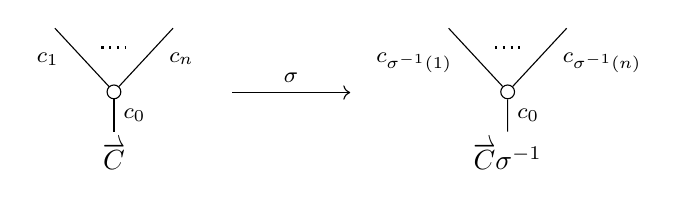
\begin{tikzpicture}
[grow=up,auto,level distance=2.3em,every node/.style = {font=\footnotesize},dummy/.style={circle,draw,inner sep=0pt,minimum size=1.75mm}]

\node at (0,0) [font=\normalsize]{$\vect{C}$}
child{node [dummy] {}
	child{
		edge from parent node [swap,near end] {$\mathfrak c_n$} node [name=Kn] {}}
	child{
		edge from parent node [near end] {$\mathfrak c_1$}
		node [name=Kone,swap] {}}
	edge from parent node [swap] {$\mathfrak c_0$}
};
\draw [dotted,thick] (Kone) -- (Kn) ;
\node at (5,0) [font=\normalsize] {$\vect{C} \sigma^{-1}
	$}
child{node [dummy] {}
	child{
		edge from parent node [swap,near end] {$\mathfrak c_{\sigma^{-1}(n)}$} node [name=Kn] {}}
	child{
		edge from parent node [near end] {$\mathfrak c_{\sigma^{-1}(1)}$}
		node [name=Kone,swap] {}}
	edge from parent node [swap] {$\mathfrak c_0$}
};
\draw [dotted,thick] (Kone) -- (Kn) ;

\draw[->] (1.5,0.8) -- node{$\sigma$} (3,0.8);
\end{tikzpicture}
\end{equation}
Alternatively,
$\mathfrak{C}$-corollas can be represented simply as
strings in $\mathfrak{C}$,
which we call $\mathfrak{C}$-profiles
(cf. Remark \ref{MAPSPTRANS REM}).
In profile notation, 
\eqref{CSYM EQ2} then becomes
\begin{equation}\label{CSYM EQ1}
\vect{C} =
(\mathfrak c_1, \dots, \mathfrak c_n; \mathfrak c_0) \xrightarrow{\sigma} (\mathfrak c_{\sigma^{-1}(1)}, \dots, \mathfrak c_{\sigma^{-1}(n)}; \mathfrak c_0)
= \vect{C} \sigma^{-1}.
\end{equation}
For this reason, we also refer to 
$\Sigma_{\mathfrak{C}}$ as the 
$\mathfrak{C}$-symmetric category,

Lastly, we note that the notation
$\vect{C} \sigma^{-1}$ used above
comes from the natural right action of $\Sigma_n$
on $\mathfrak{C}$-profiles of arity $n$ via
$
(\mathfrak c_1, \dots, \mathfrak c_n; \mathfrak c_0) \sigma
=
(\mathfrak c_{\sigma(1)}, \dots, \mathfrak c_{\sigma(n)}; \mathfrak c_0)$.


\begin{definition}\label{SSYM DEF}
	The category $\mathsf{sSym}$ of \textit{simplicial symmetric sequences} has:
\begin{itemize}
	\item objects given by pairs
	$(\mathfrak C, X)$ with $\mathfrak{C} \in \mathsf{Set}$
	a set of colors and
	$\Sigma_{\mathfrak C}^{op} \xrightarrow{X}\sSet$
	a functor; 
	\item a map
	$(\mathfrak{C},X) \to (\mathfrak{D},Y)$
	given by a map of colors
	$\varphi \colon \mathfrak{C} \to \mathfrak{D}$
	and $\Phi$ as below.
\begin{equation}
\begin{tikzcd}[row sep = tiny, column sep = 45pt]
	\Sigma_{\mathfrak{C}}^{op} \arrow[dr, "X"{name=U}] 
	\arrow{dd}[swap]{\varphi}
\\
	& \mathsf{sSet}
\\
	|[alias=V]| \Sigma_{\mathfrak{D}}^{op} \arrow[ur, "Y"']
\arrow[Leftarrow, from=V, to=U,shorten >=0.25cm,shorten <=0.25cm, swap,"\Phi"]
\end{tikzcd}
\end{equation}
\end{itemize} 
\end{definition}

More explicitly,
we note specifying \eqref{CSYM EQ2} to a map
$\vect{C} \sigma \to \vect{C}$ in $\Sigma_{\mathfrak{C}}$,
one has that a symmetric sequence
$X \colon \Sigma_{\mathfrak{C}}^{op} \to \mathsf{sSet}$
has structure maps
\begin{equation}\label{SSYMSTMAP EQ}
	X(\vect{C}) = 
	X(\mathfrak c_1, \dots, \mathfrak c_n; \mathfrak c_0) \xrightarrow{\simeq} 
	X(\mathfrak c_{\sigma(1)}, \dots, \mathfrak c_{\sigma(n)}; \mathfrak c_0) =	
	X(\vect{C}\sigma)
\end{equation}
for $\vect{C}$ of arity $n$ and $\sigma \in \Sigma_n$.



The free operad monad $\mathbb{F}$
is then a monad on $\mathsf{sSym}$ which,
when evaluated on $X \colon \Sigma_{\mathfrak{C}}^{op} \to \mathsf{sSet}$,
is given by the left Kan extension
(the real challenge, of course, is that of defining the multiplication
$\mathbb{F}\mathbb{F} \Rightarrow \mathbb{F}$)
\begin{equation}\label{FREEOP_EQ}
\begin{tikzcd}[column sep = 150pt]
	\Omega^{0,op}_{\mathfrak{C}}
	\arrow[d, "\mathsf{lr}^{op}"']
	\arrow[r, 
	"\vect{T} \mapsto \prod_{v \in \boldsymbol{V}(T)} X(\vect{T}_v)"{name=U}]
&
	\mathsf{sSet}
\\
	|[alias=V]|
	\Sigma^{op}_{\mathfrak{C}}
	\arrow[ur, "\Lan = \mathbb F X"']
	\arrow[Leftarrow, from=V, to=U,shorten >=0.25cm,shorten <=0.25cm]
\end{tikzcd}
\end{equation}
The category 
$\mathsf{sOp}$ of \emph{colored simplicial operads}
can then be described as the category of 
$\mathbb{F}$-algebras on $\mathsf{sSym}$.
For $G$ a finite group, we then write
$\mathsf{sOp}^G$ (resp. $\mathsf{sSym}^G$)
for the category of 
$G$-objects on 
$\mathsf{sOp}$ ($\mathsf{sSym}$)
which we call the category of
\emph{$G$-equivariant colored simplicial operads
(symmetric sequences)}.
Note that, by abstract nonsense,
$\mathbb{F}$
induces a monad on $\mathsf{sSym}^G$
whose category of algebras is $\mathsf{sOp}^G$.


Mirroring \eqref{COLORSET EQ}
we now have \emph{color set functors}
\begin{equation}\label{OPERCOLFUN EQ}
	\mathsf{sSym} \xrightarrow{\mathfrak{C}_{\bullet}} \mathsf{Set}
\qquad
	\mathsf{sOp} \xrightarrow{\mathfrak{C}_{\bullet}} \mathsf{Set}
\qquad
	\mathsf{sSym}^G \xrightarrow{\mathfrak{C}_{\bullet}} \mathsf{Set}^G
\qquad
	\mathsf{sOp}^G \xrightarrow{\mathfrak{C}_{\bullet}} \mathsf{Set}^G.
\end{equation}

\begin{remark}\label{CTTCOLSET REM}
	Replacing $\mathsf{sSet}$ with 
	$\mathsf{Set}$
	in Definition \ref{SSYM DEF}
	and \eqref{FREEOP_EQ}
	one recovers the analogue non-simplicial categories
	$\mathsf{Sym}$, 
	$\mathsf{Op}$, 
	$\mathsf{Sym}^G$, 
	$\mathsf{Op}^G$. 
%	
	As is well known, there is then a fully faithful inclusion
	$\mathsf{sOp} \subset \mathsf{Op}^{\Delta^{op}}$
	as those simplicial objects with a constant set of colors.
\end{remark}


The color set functors above are all 
Grothendieck fibrations and, moreover, the monad 
$\mathbb{F}$ is suitably compatible with these fibrations.
In \cite{BP_HGOP} the fibration perspective 
is used to describe the fibers 
$\mathsf{sSym}^G_{\mathfrak{C}}$, 
$\mathsf{sOp}^G_{\mathfrak{C}}$
of those objects with a fixed $G$-color set $\mathfrak{C}$
and maps which are the identity on colors. 
However, here we will be able to make do with a more elementary approach.

If $\mathfrak{C}$ is a $G$-set of colors, 
one has a left $G$-action of $\mathfrak{C}$-profiles.
Then, if $X \in \mathsf{sSym}^G$
has colors $\mathfrak{C}_X =\mathfrak{C}$,
on has, generalizing
\eqref{SSYMGSTMAP EQ},
that $X$ has structure maps
\begin{equation}\label{SSYMGSTMAP EQ}
X(\vect{C}) = 
X(\mathfrak c_1, \dots, \mathfrak c_n; \mathfrak c_0) \xrightarrow{\simeq} 
X(g\mathfrak c_{\sigma(1)}, \dots, g \mathfrak c_{\sigma(n)}; g \mathfrak c_0) =	
X(g \vect{C}\sigma)
\end{equation}
for $\vect{C}$ a $\mathfrak{C}$-profile of arity $n$
and
$(g,\sigma) \in G \times \Sigma^{op}_n$.

Note that, implicit in the $g \vect{C} \sigma$ notation in
\eqref{SSYMGSTMAP EQ}
is the fact that $G \times \Sigma_n^{op}$
has a left action on 
$\mathfrak{C}$-profiles of arity $n$.
As such, given a subgroup
$\Gamma \leq G \times \Sigma_n^{op}$
and $\vect{C}$ of arity $n$, we say that 
\emph{$\Gamma$ stabilizes $\vect{C}$} 
if 
$g \vect{C} \sigma = \vect{C}$
for all $(g,\sigma) \in \Gamma$.
In particular, 
\eqref{SSYMGSTMAP EQ}
then implies that whenever $\Gamma$ stabilizes $\vect{C}$
and for
$X\in \mathsf{sSym}^G$
(resp.
$\O \in \mathsf{sOp}^G$)
with $G$-color set $\mathfrak{C}$,
the level
$X(\vect{C})$
(resp. $\O(\vect{C})$)
has an action by $\Gamma$.


\begin{notation}\label{SIGFREE NOT}
	For $x \in X(\vect{C})$
	with $\vect{C}$ of arity $n$ and 
	$(g,\sigma) \in G \times \Sigma_n^{op}$
	we write
	$gx\sigma \in X(g \vect{C} \sigma)$
	for the image of $x$ under 
	\eqref{SSYMGSTMAP EQ}.
	Note that this defines an action of
	$G \times \Sigma_n^{op}$
	on $\coprod_{\vect{C} \text{ of arity }n} X(\vect{C})$.
	
	Moreover, if $x \sigma = x$ only when $\sigma = id$ then we say 
	$x$ is \emph{$\Sigma$-free}.
\end{notation}




\begin{remark}\label{SYMGCPRESH REM}
	Let $\mathcal{G}_{\mathfrak{C}}$
	denote the groupoid with objects the 
	$\mathfrak{C}$-signatures
	and arrows 
	$\vect{C} \to g \vect{C} \sigma$
	for $\vect{C}$ of arity $n$
	and $(g,\sigma) \in G \times \Sigma^{op}_n$.
	In other words, 
	$\mathcal{G}_{\mathfrak{C}}$
	is the coproduct over $n\geq 0$ of the action groupoids 
	for the actions of
	$G \times \Sigma^{op}_n$
	on $n$-ary signatures
	(alternatively, in 
	\cite{BP_HGOP} 
	we use an alternative description
	$\mathcal{G}_{\mathfrak{C}}
	= G \ltimes \Sigma_{\mathfrak{C}}^{op}$;
	see \cite[Prop. 2.52]{BP_HGOP}).
%	
	Equation \eqref{SSYMGSTMAP EQ} then identifies 
	$\mathsf{sSym}^G_{\mathfrak{C}} \simeq 
	\mathsf{sSet}^{\mathcal{G}_{\mathfrak{C}}}$.	
\end{remark}








Before describing the model structure on $\mathsf{sOp}^G$
we need to recall two more ingredients.

First, 
a subgroup $\Gamma \leq G \times \Sigma_n^{op}$
is called a \emph{$G$-graph subgroup}
if $\Gamma \cap \Sigma_n^{op} = \{*\}$.
Equivalently, it is straightforward to show
that $\Gamma$ must be of the form 
$\Gamma = \sets{(h,\phi(h)^{-1})}{h \in H}$
for some subgroup $H \leq G$
and homomorphism $\phi \colon H \to \Sigma_n$.

Second, one has functors
\[
	\mathsf{sOp} \xrightarrow{\pi_0}
	\mathsf{Op} \xrightarrow{j^{\**}}
	\mathsf{Cat}
\]
where $\pi_0$ is computed levelwise,
i.e. 
$(\pi_0 \O)(\vect{C}) = 
\pi_0(\O(\vect{C}))$
and
$j^{\**}$ forgets non-unary operations.


Generalizing \cite{Ber07b,CM13b},
we show in \cite{BP_HGOP}
that $\mathsf{sOp}^G$ 
has a Dwyer-Kan style model structure.
More precisely, we have the following result, which is
\cite[Thm. III]{BP_HGOP},
with the alternative characterization of fibrations 
provided by 
\cite[Prop. 4.78]{BP_HGOP}.



\begin{theorem}\label{SOPG_THM}
      The category $\sOp^G$ has a cofibrantly generated model structure with weak equivalences (resp. fibrations) those maps
      $F \colon \O \to \P$ such that:
\begin{itemize}
\item $F$ is \emph{fully faithful} (resp. a \emph{local fibration}), i.e. the induced maps
	\begin{equation}\label{DKEQUIV_EQ}
		\O ( \vect{C})^\Gamma \longto 
		\P(F \vect{C})^\Gamma
	\end{equation}
	are Kan equivalences (resp. Kan fibrations) in $\sSet$
	for all $\mathfrak C_\O$-signatures $\vect C = (\mathfrak c_1, \dots, \mathfrak c_n; \mathfrak c_0)$
	and all graph subgroups $\Gamma \leq G \times \Sigma_n^{op}$ which stabilize $\vect C$;
\item $F$ is \emph{essentially surjective} (resp. an \emph{isofibration}), i.e. the induced maps of usual categories
	\begin{equation}\label{ESSSURJ EQ}
		j^{\**}\pi_0 \O^H \longto j^{\**}\pi_0 \P^H
	\end{equation}
	are essentially surjective (resp. isofibrations) for all $H \leq G$.
\end{itemize}
\end{theorem}



	For a fixed $G$-set of colors $\mathfrak{C}$,
	the 
	fixed color symmetric sequences
	category
	$\mathsf{sSym}_{\mathfrak{C}}^G$
	admits an auxiliary model structure where
	(adapting \eqref{DKEQUIV_EQ})
	$X \to Y$ is a (trivial) fibration
	iff 
	$X(\vect{C})^{\Gamma} \to Y(\vect{C})^{\Gamma}$
	is a (trivial) Kan fibration.
	For instance, using the identification
	$\mathsf{sSym}^{G}_{\mathfrak{C}}
	\simeq \mathsf{sSet}^{\mathcal{G}_{\mathfrak{C}}}$
	from Remark \ref{SYMGCPRESH REM},
	this is the model structure
	from \cite[Prop. 3.17]{BP_HGOP}
	with respect to the family of 
	$\mathcal{F}^{\Gamma}$
	such that
	$\mathcal{F}^{\Gamma}_{\vect{C}}$
	consists of the graph subgroups stabilizing $\vect{C}$
	(here we use the fact that the automorphism group of 
	an $n$-ary signature $\vect{C}$ in 
	$\mathcal{G}_{\mathfrak{C}}$
	can be naturally viewed as a subgroup of 
	$G \times \Sigma_n^{op}$).




\begin{proposition}\label{SSYMCOFCH PROP}
	Let $f \colon A \to B$ be a map in
	$\mathsf{sSym}^G_{\mathfrak{C}} \simeq \mathsf{sSet}^{\mathcal{G}_{\mathfrak{C}}}$.
	The following are equivalent:
\begin{enumerate}
	\item[(i)] $f$ is a cofibration;
	\item[(ii)] $f$ is a monomorphism and the stabilizer of every
	$x \in B \setminus f(A)$
	is a graph subgroup;
	\item[(iii)] $f$ is a monomorphism and every 
	$x \in B \setminus f(A)$ is $\Sigma$-free
	(cf. Notation \ref{SIGFREE NOT}).
\end{enumerate}
\end{proposition}

\begin{proof}
By \cite[Rem. 3.14]{BP_HGOP}
the generating cofibrations in 
$\mathsf{sSym}^G_{\mathfrak{C}}$
then have the form
$\mathcal{G}_{\mathfrak{C}}
(\vect{C},-)/\Gamma \cdot (\partial \Delta[k] \to \Delta[k])$
with $\Gamma \in \mathcal{F}^{\Gamma}_{\vect{C}}$,
$k \geq 0$,
so that (i) $\Leftrightarrow$ (ii)
follows by adapting 
\cite[Prop. 2.16]{Ste16}
or
\cite[Prop. 6.5]{Per18}.
(ii) $\Leftrightarrow$ (iii)
is straightforward.
\end{proof}



In light of (iii) in the previous result,
a color fixed map of operads
$\O \to \mathcal{P}$
such that the underlying map of symmetric sequences is a cofibration
is called a \emph{$\Sigma$-cofibration}.
%
Combining Proposition \ref{SSYMCOFCH PROP} with \cite[Prop. 3.63]{BP_HGOP} (also, see 
\cite[Prop. 4.11(ii)]{BP_HGOP})
yields the following.


\begin{proposition}\label{COPOFSIGCOF PROP}
	If $f \colon \O \to \mathcal{P}$
	is a color fixed map in $\mathsf{sOp}^G$
	and $\O$ is $\Sigma$-cofibrant
	then $f$ is a $\Sigma$-cofibration.
	In particular, cofibrant operads are $\Sigma$-cofibrant.
\end{proposition}




We next recall the 
\emph{operadification-nerve functor}
adjunctions
\begin{equation}\label{TAUNER EQ}
	\tau\colon \mathsf{dSet}
	\rightleftarrows
	\mathsf{Op} \colon N
\qquad
	\tau\colon \mathsf{PreOp}
	\rightleftarrows
	\mathsf{sOp} \colon N.
\end{equation}
where we note that the rightmost adjunction 
is induced by applying the leftmost adjunction
to each simplicial level
(indeed, by Definition \ref{PREOP DEF} 
Remark \ref{CTTCOLSET REM}
both $\mathsf{PreOp}$ and $\mathsf{sOp}$
are characterized by demanding that
the color sets on all simplicial levels are
are the same).

To describe the nerve $N$, 
we need to recall the operad
$\Omega(F) \in \mathsf{Op}$
freely determined by a forest $F \in \Phi$.
Explicitly, 
$\Omega(F)$ is the $\boldsymbol{E}(F)$-colored operad
which, when evaluated on
a $\boldsymbol{E}(F)$-colored corolla
$\vect{C} = 
(C,\mathfrak{c} \colon \boldsymbol{E}(C) \to \boldsymbol{E}(F))$,
is given by
\begin{equation}\label{OMEGADEF_EQ}
\Omega(F)(\vect C) =
	\begin{cases}
		\** \qquad & 
		\mbox{if
			$\mathfrak{c} \colon \boldsymbol{E}(C) \to \boldsymbol{E}(F)$
			defines a map $C \to F$ in $\Phi$}
	\\
		\varnothing & \text{otherwise.}
	\end{cases}
\end{equation}
We note that, since all levels of 
$\Omega(F)$ are either $\**$ or $\emptyset$,
there is always at most one possible way to compose operations,
and hence at most one possible operad structure on $\Omega(F)$.
That the operad structure indeed exists 
(i.e. that composition is always defined)
is a consequence of the observation that,
for any tree $U\in \Omega$,
a coloring
$\mathfrak{c} \colon \boldsymbol{E}(U) \to \boldsymbol{E}(F)$
defines a map
$U \to F$ in $\Phi$
iff
the restrictions
$\mathfrak{c}_v \colon \boldsymbol{E}(U_v) \to \boldsymbol{E}(F)$
define maps
$U_v \to F$ in $\Phi$
for all vertices $v \in \boldsymbol{V}(U)$.


We will also make use of an alternative description of $\Omega(F)$, as follows.

First, if $\vect{C}\in \Sigma_{\mathfrak{C}}$ is a
$\mathfrak{C}$-corolla,
we denote its representable functor as 
$\Sigma_{\mathfrak C}[\vect C] =
\Sigma_{\mathfrak C}^{op}(\vect C, -)$ in 
$\Sym_{\mathfrak C} = \mathsf{Set}^{\Sigma^{op}_{\mathfrak{C}}}$.
Second, for
$\vect{F}\in \Phi_{\mathfrak{C}}$ a
$\mathfrak{C}$-forest, 
we extend the 
$\Sigma_{\mathfrak C}[-]$ notation via
\[
	\Sigma_{\mathfrak C}[\vect F] = \sideset{}{^{\mathfrak C}}\coprod_{v \in \boldsymbol{V}(F)} \Sigma_{\mathfrak C}[\vect F_v],
\]
where $\amalg^{\mathfrak C}$ denotes the coproduct
in $\Sym_{\mathfrak C}$ (rather than in the larger category $\Sym$).
Third, for 
$F \in \Phi$
an (uncolored) forest we write
$F^{\tau}$ for $F$ together with its tautological 
$\boldsymbol{E}(F)$-coloring, i.e.
$F^{\tau} = 
(F,\mathfrak{t}\colon \boldsymbol{E}(F) \xrightarrow{=} \boldsymbol{E}(F))$,
and abbreviate
$\Sigma_{\tau}[F] = \Sigma_{\boldsymbol{E}(T)}[F^{\tau}]$.
All together, one then has an identification
\begin{equation}\label{OMFFREE EQ}
	\Omega(F) = \mathbb{F} \Sigma_{\tau}[F]
\end{equation}
which, informally, says that 
``$\Omega(F)$ is freely generated by the vertices of $F$''.

For $\O \in \mathsf{Op}$
the nerve $N \O \in \mathsf{dSet}$ from \eqref{TAUNER EQ}
is then described by
\[
	(N \O) (U) = \mathsf{Op}(\Omega(U),\O),\qquad U \in \Omega
\]
while $\tau\colon \mathsf{dSet} \to \mathsf{Op}$
is the unique colimit preserving functor such that
$\tau(\Omega[U]) \to \Omega(U)$.



We now recall \cite[Prop. 5.3 and Thm. 6.1]{MW09}
that the nerve
$N \colon \mathsf{\O} \to \mathsf{dSet}$
is then a fully faithful inclusion
whose (essential) image can be characterized
as those
dendroidal sets $X \in \mathsf{dSet}$
with the strict right lifting property against inner horn inclusions
$\Lambda^e[U] \to \Omega[T]$ for $U\in\Omega,e\in \boldsymbol{E}(U)$.
Next,
following either \cite[Prop. 2.5 and Cor. 2.6]{CM13a}
or \cite[Props. 3.22 and 3.31]{BP_edss},
this is in turn equivalent to the strict right lifting property of $X$
against Segal core inclusions
$Sc[U] \to \Omega[T]$ for $U \in \Omega$,
which is in turn equivalent to the strict Segal condition
(cf. Definition \ref{SEGCOLCHAR DEF}) below,
demanding that the maps
\begin{equation}\label{STRSEGCON EQ}
	X(U)
	\xrightarrow{\simeq}
	X(Sc[U]),
	\quad
	U \in \Omega
\qquad \qquad
	X_{\mathfrak{c}}(U) 
	\xrightarrow{\simeq}
	\prod_{v \in \boldsymbol{V}(U)}
	X_{\mathfrak{c}_v}(U_v),
	\quad
	U \in \Omega,
	\mathfrak{c} \colon 
	\boldsymbol{E}(U) \to X(\eta)
\end{equation}
are all isomorphisms.
Moreover, one then has the following alternate formula for the nerve
$N \O$ evaluated at
$U\in \Omega,
\mathfrak{c} \colon \boldsymbol{E}(U) \to \mathfrak{C}_{\O}$.
\begin{equation}\label{ALTNER EQ}
	(N \O)_{\mathfrak{c}} (U) 
	= 
	\prod_{v \in \boldsymbol{E}(U)}
	\O(U_v,\mathfrak{c}_v)
	=
	\prod_{v \in \boldsymbol{E}(U)}
	\O(\vect{U}_v).
\end{equation}



To describe the generating (trivial) cofibrations of 
the model structure in Theorem \ref{SOPG_THM}
we will make use of a fibered simplicial tensoring on
$\mathsf{sOp}^G$
which is closely related to the analogue tensoring on
$\mathsf{PreOp}^G$
from \S \ref{FIBTENS_SEC}.

First, for $\O \in \mathsf{sOp}^G_{\mathfrak{C}}$
and 
$K \in \mathsf{sSet}$
we define the \emph{fiber cotensor}
$\{K,\O\}_{\mathfrak{C}_{\bullet}} 
\in \mathsf{sOp}^G_{\mathfrak{C}}$
via the pointwise simplicial cotensor, i.e.
\begin{equation}\label{KOCOPER EQ}
	\set{K, \O}_{\mathfrak{C}_{\bullet}} (\vect C) = \O(\vect C)^K.
\end{equation}


\begin{remark}\label{NERTENID REM}
	The fact that 
	$\set{K, \O}_{\mathfrak{C}_{\bullet}}$
	as described above has an operad structure
	can be seen by considering nerves. 
	Indeed, 
	one readily checks that the strict Segal condition
	\eqref{STRSEGCON EQ} for $N\O$
	implies the same condition for 
	the preoperad
	$\{K,N \O\}_{\mathfrak{C}_{\bullet}}$
	(defined as in \eqref{EASYCOTEN EQ}).
	Thus, \eqref{KOCOPER EQ}
	describes the levels
	of the unique (up to isomorphism) operad
	$\set{K, \O}_{\mathfrak{C}_{\bullet}}$
	such that
	$N \set{K, \O}_{\mathfrak{C}_{\bullet}} 
	\simeq
	\set{K, N \O}_{\mathfrak{C}_{\bullet}}$.
\end{remark}



Next, we turn to the \emph{fiber tensor} 
$(-)\otimes_{\mathfrak{C}_{\bullet}} K$
adjoint to \eqref{KOCOPER EQ}.
First, note that 
\eqref{KOCOPER EQ}
still makes sense 
at the level of symmetric sequences, i.e. 
with 
$\O \in \mathsf{sOp}^G_{\mathfrak{C}}$
replaced with
$X \in \mathsf{sSym}^G_{\mathfrak{C}}$.
Then, at the level of symmetric sequences, the left adjoint construction
$X \times K \in \mathsf{sSym}^G_{\mathfrak{C}}$
is simply given pointwise by
$(X \times K)(\vect{C}) = X(\vect{C}) \times K$.
It is now formal that, 
on a free operad $\mathbb{F} X$,
the tensor $\mathbb{F} X \otimes_{\mathfrak{C}_{\bullet}} K$
adjoint to \eqref{KOCOPER EQ} is given by 
$(\mathbb{F} X) \otimes_{\mathfrak{C}_{\bullet}} K
= \mathbb{F} (X \times K)$
so that,
for a general $\O \in \mathsf{sOp}^G$
(which has a standard description
$\O \simeq coeq (\mathbb{F}\mathbb{F}\O \rightrightarrows \mathbb{F}\O)$
as a coequalizer of free algebras)
it is given by
\[
\mathcal{O} \otimes_{\mathfrak{C}_{\bullet}} K
\simeq
coeq 
\left(
\mathbb{F} (\mathbb{F} \O \times K) 
\rightrightarrows \mathbb{F} (\O \times K) 
\right).
\]
\begin{remark}\label{BYHAND2 REM}
	In \cite[\S 7.1]{CM13b}, 
	the objects $\Omega(T)  \otimes_{\mathfrak{C}_{\bullet}} K$
	were denoted $T[K]$ and built by hand.
\end{remark}


\begin{remark}
	The analogues of Remarks \ref{TENSCOADJ REM},
	\ref{NOTTWOVARADJ REM}
	apply mutatis mutandis to the operadic fiber tensor.
%	
	In particular, one has that the canonical map
\begin{equation}\label{COCARTAR EQ}
	\amalg_i \O \otimes_{\mathfrak{C}_{\bullet}} K_i
	\to
	\O \otimes_{\mathfrak{C}_{\bullet}} (\amalg_i K_i)
\end{equation}
	is a cocartesian arrow over the fold map
	$\amalg_i \mathfrak{C} \to \mathfrak{C}$.
\end{remark}



\begin{proposition}\label{TAUOTIMES_PROP}
	For all $X \in \mathsf{PreOp}^G$ and $K \in \sSet$, 
	one has a natural identification
	\[\tau(X \otimes_{\mathfrak{C}_{\bullet}} K) \simeq \tau(X) \otimes_{\mathfrak{C}_{\bullet}} K\]
	with the first (resp. second) $\otimes_{\mathfrak{C}_{\bullet}}$ is 
	the fiber simplicial tensoring of $\mathsf{PreOp}^G$ 
	(resp. $\sOp^G$).
\end{proposition}

\begin{proof}
	This is equivalent to the 
	already established (cf. Remark \ref{NERTENID REM}) adjoint identification
	$
	N \{K,\O\}_{\mathfrak{C}_{\bullet}}
	\simeq
	\{K,N \O\}_{\mathfrak{C}_{\bullet}} 
	$
	for $\O \in \mathsf{sOp}^G$.	
\end{proof}



\begin{remark}
	Proposition \ref{TAUOTIMES_PROP} is a slight generalization of 
	\cite[Prop. 7.2]{CM13b},
	which establishes the case
	$X = \Omega[U]$, $U\in \Omega$
	by direct inspection
	(cf. Remarks \ref{BYHAND1 REM},\ref{BYHAND2 REM}).
\end{remark}



\begin{remark}\label{SIGMATAUQUOT REM}
Let $\Gamma \leq G \times \Sigma_n^{op}$
be the graph subgroup given by
$\Gamma = \{(h,\phi(h)^{-1})|h\in H\}$
for $H\leq G$, $\phi\colon H \to \Sigma_n$.
Writing
$C_{n}$ for the $n$-corolla, 
$\phi$ defines a left $H$-action on $C_{n}$,
so that one obtains an associated
$G$-corolla $C = G \cdot_{H} C_{n}$.
It is then straightforward to check that there are natural identifications
(here we view the natural 
left $G^{op}\times \Sigma_n$-action on 
$G \cdot C_{n}$ has a 
right $G\times \Sigma_n^{op}$-action)
\begin{equation}\label{SIGMATAUQUOT EQ}
	(G \cdot C_{n})/\Gamma
\simeq
	G \cdot_H C_{n}
= 
	C
\qquad
	\Sigma_{\tau}[G \cdot C_{n}]/\Gamma
\simeq
	\Sigma_{\tau}[G \cdot_H C_{n}]
= 
	\Sigma_{\tau}[C]
\end{equation}
in $\Phi^G_{\bullet}$ and $\mathsf{Sym}^G$, respectively.
\end{remark}


We need one final ingredient to describe the generating sets of maps for the model structure on
$\mathsf{sOp}^G$
(cf. \cite[Def. 4.4]{BP_HGOP}).


\begin{definition}
	Let $\widetilde{[1]}$ denote the free isomorphism category,
	i.e. the contractible groupoid with two objects $0,1$.
%		
	An \textit{interval} is a cofibrant simplicial category $\mathbb I \in \mathsf{sCat}_{\set{0,1}}$ equivalent to $\widetilde{[1]}$.
\end{definition}

%The canonical example is $W_!N\widetilde{[1]}$, with the equivalence given by the counit of the adjunction.

\begin{remark}
	Specifying \cite[Def. 4.19]{BP_HGOP}
	for $\mathsf{sSet}$, we can rewrite the notation therein via
\[
	\mathbb{F}
	\left(\Sigma_{\tau}[G \cdot C_{n}]/\Gamma \cdot f\right)
\simeq
	\mathbb{F}
	\left(\Sigma_{\tau}[C] \cdot f\right)
\simeq
	\mathbb{F}
	\left(\Sigma_{\tau}[C] \right) \otimes_{\mathfrak{C}_{\bullet}} f
\simeq 
	\Omega(C) \otimes_{\mathfrak{C}_{\bullet}} f
\]
where the first identification is
\eqref{SIGMATAUQUOT EQ},
the second follows by definition of
$\otimes_{\mathfrak{C}_{\bullet}}$,
and the third is \eqref{OMFFREE EQ}.
We thus have that the generating cofibrations in $\mathsf{sOp}^G$
are the maps
	\begin{itemize}
		\item[(C1)] $\emptyset \to G/H \cdot \Omega(\eta)$ for $H \leq G$
		\item[(C2)] $\Omega(C) \otimes_{\mathfrak{C}_{\bullet}} (\partial \Delta[m] \to \Delta[m])$
		for $C \in \Sigma_G$, $m \geq 0$.
	\end{itemize}
	while the generating trivial cofibrations are 
	(for the countability condition, see \cite[Rem. 4.17]{BP_HGOP})
	\begin{itemize}
		\item[(A1)] 
		$G/H \cdot \left(\eta \to \mathbb{G}\right)$ 
		for $H \leq G$ and $\mathbb G$ an interval with countably many simplices.
		\item[(A2)] 
		$\Omega(C) \otimes_{\mathfrak{C}_{\bullet}} (\Lambda^k[m] \to \Delta[m])$
		for $C \in \Sigma_G$, $m \geq 1$, $0 \leq k \leq m$.
	\end{itemize}
\end{remark}

In (C2),(A2) above 
the group $G$ acts only on $\Omega(C)$
and not on the featured simplicial sets.
The following lemma will allow us to consider the case where the simplicial sets also have a $G$-action.

\begin{lemma}
	\label{OPTENSCOF_LEM}
	For $C \in \Sigma_G$ and $A \to B$ a genuine (trivial) cofibration in $\sSet^G$,
	$\Omega(C) \otimes_{\mathfrak{C}_{\bullet}} (A \to B)$ is a (trivial) cofibration in $\sOp^G$.
\end{lemma}

\begin{proof}
	Since $\Omega(C) \otimes (-) \colon \sSet^G \to \sOp^G_{\boldsymbol{E}(T)}$ preserves colimits, 
	it suffices to consider the case 
	$(A \to B) = G/H \cdot (K \to L)$ for $K \to L$ a (trivial) cofibration in $\sSet$.
	Now consider the following diagram.
\begin{equation}
\begin{tikzcd}[column sep = small, ampersand replacement = \&]
	\left(G/H \cdot \Omega(C)\right) \otimes_{\mathfrak{C}_{\bullet}} K 
	\arrow[r] \arrow[d]
\&
	\Omega(C) \otimes_{\mathfrak{C}_{\bullet}} \left(G/H \cdot K\right)
	\arrow[d]
\\
	\left(G/H \cdot \Omega(C)\right) \otimes_{\mathfrak{C}_{\bullet}} L
	\arrow[r] 
\&
	\Omega(C) \otimes_{\mathfrak{C}_{\bullet}} \left(G/H \cdot L\right)
\end{tikzcd}
% }
\end{equation}
By \eqref{COCARTAR EQ} the horizontal arrows are cocartesian, while the vertical arrows fix colors, 
so this is a pushout square.
The result now follows since 
$G/H \cdot \Omega(C)$ decomposes as a coproduct 
$\amalg_i \Omega(C_i)$ with $C_i\in \Sigma_G$.
\end{proof}



%\begin{lemma}[cf. Lemma \ref{OMEGATTAME_LEM}]
%	For all $T \in \Omega_G$, $\Omega(T) \in \sOp^G$ is cofibrant.
%\end{lemma}
%
%\begin{proof}
%	This follows since the square below is a pushout in $\sOp^G$,
%	with $\coprod_{\boldsymbol{E}(T)} \Omega(\eta)$ cofibrant by (C1),
%	while the left vertical map is a cofibration by (C2) with $n=0$.
%	\[
%	\begin{tikzcd}
%	\displaystyle{
%		\coprod_{Gv \in \boldsymbol{V}_G(T)} \partial \Omega(T_{Gv})
%	}
%	\arrow[d] \arrow[r]
%	&
%	\displaystyle{
%		\coprod_{\boldsymbol{E}(T)} \Omega(\eta)
%	}
%	\arrow[d]
%	\\
%	\displaystyle{
%		\coprod_{Gv \in \boldsymbol{V}_G(T)} \Omega(T_{Gv})
%	}
%	\arrow[r]
%	&
%	\Omega(T)
%	\end{tikzcd}
%	\]
%\end{proof}













\subsection{Quillen equivalence between preoperads and operads}
\label{PREOPOPEQUIV SEC}

Our goal in this subsection is to prove
Theorem \ref{PREQUIEQUIV THM},
showing the Quillen equivalence between
preoperads $\mathsf{PreOp}^G$
and operads $\mathsf{sOp}^G$.
The key to proving this result is given by 
Lemma \ref{UNITEQUIV LEM}
and the subsequent
Corollary \ref{KEYEQUIV COR},
which allow us to understand the counit of the adjunction.
These latter results in turn depend on the following key 
result, whose proof is deferred to \S \ref{KEYRES SEC}.


\begin{lemma}\label{KEYPRVAR LEM}
	Suppose that $\mathcal{O} \in \mathsf{Op}^{G}$
	is $\Sigma$-cofibrant.
	Further, let $C \in \Sigma_G$ be any $G$-corolla,
	$r \geq 1$ a positive integer and consider 
	a pushout in $\mathsf{Op}^{G}$ of the form
\begin{equation}\label{PUSHOUTPROPVAR EQ}
	\begin{tikzcd}
	\partial \Omega(C)^{\amalg r} \ar{r} \ar{d} 
	& \mathcal{O} \ar{d}
\\
	\Omega(C)^{\amalg r} \ar{r} & \mathcal{P}.
	\end{tikzcd}
\end{equation}
	Then the induced map
\begin{equation}\label{ANODYNEVAR EQ}
	\Omega[C]^{\amalg r} 
	\amalg_{\partial \Omega[C]^{\amalg r}} N\mathcal{O} \to N\mathcal{P}
\end{equation}
	is $G$-inner anodyne.
\end{lemma}

\begin{remark}\label{KEYPRVAR REM}
	Both \eqref{PUSHOUTPROPVAR EQ} and \eqref{ANODYNEVAR EQ}
	are unchanged if the copowers $(-)^{\amalg r}$ in 
	$\mathsf{Op}^G$, $\mathsf{dSet}^G$
	are replaced with fibered copowers 
	$(-)^{\amalg_{\mathfrak{C}_{\bullet}} r} \simeq 
	(-) \otimes_{\mathfrak{C}_{\bullet}} \{1,\cdots,r\}$
	in 
	$\mathsf{Op}^G_{\boldsymbol{E}(C)}$,
	$\mathsf{dSet}^G_{\boldsymbol{E}(C)}$.
	
	Moreover, since 
	$\partial \Omega(C) = \Omega(C) \otimes_{\mathfrak{C}_{\bullet}} \emptyset$,
	one is moreover free to replace
	the left vertical map in \eqref{PUSHOUTPROPVAR EQ}
	with 
	$\Omega(C) \otimes_{\mathfrak{C}_{\bullet}} K
	\to
	\Omega(C) \otimes_{\mathfrak{C}_{\bullet}} L$
	for $K\to L$ any inclusion of sets.
\end{remark}


\begin{remark}
	The integer $r \geq 1$ in 
	Lemma \ref{KEYPRVAR LEM}
	is included to match our required application in Lemma \ref{UNITEQUIV LEM}.
	However, it readily follows by induction on $r$ that one needs only prove the $r=1$ case.
	Indeed, writing $\O_r$ for the pushout in 
	\eqref{PUSHOUTPROPVAR EQ}
	for each $r$,
	one has a diagram below
\begin{equation}
\begin{tikzcd}
	\Omega[C]^{\amalg r} \amalg_{\partial \Omega[C]^{\amalg r}} N\mathcal{O} \ar{r} \ar{d}
&
	N \mathcal{O}_r \ar{d}
\\
	\Omega[C]^{\amalg r+1} \amalg_{ \partial \Omega[C]^{\amalg r+1}} N \mathcal{O} \ar{r}
&
	\Omega[C] \amalg_{\partial \Omega[C]} N \mathcal{O}_r \ar{r}
&
	N \mathcal{O}_{r+1}
\end{tikzcd}
\end{equation}
	where the square is a pushout so that induction on $r$ and the $r=1$ case yield that all horizontal maps
	are $G$-inner anodyne.
	The proof of the interesting $r=1$ case will occupy the entirety of \S \ref{KEYRES SEC}.
\end{remark}





\begin{lemma}\label{UNITEQUIV LEM}
	Let $A \to B$ be a tame cofibration in $\mathsf{PreOp}^G$, 
	$\mathcal{O} \in \mathsf{sOp}^G$ a $\Sigma$-cofibrant 
	$G$-operad,
	and consider a pushout diagram in $\mathsf{sOp}^G$ of the form
\begin{equation}\label{THEPUSH EQ}
\begin{tikzcd}
	\tau A \ar{r} \ar{d} & \mathcal{O} \ar{d}
\\
	\tau B \ar{r} & \mathcal{P}
\end{tikzcd}
\end{equation}
	Then $\mathcal{O} \to \mathcal{P}$ is a $\Sigma$-cofibration and 
	\begin{equation}\label{UNITEQUIV EQ}
	B \amalg_{A} N \mathcal{O}
	\to 
	N \mathcal{P}
	\end{equation}
	is a weak equivalence.
\end{lemma}

Setting $A = \emptyset $, $\mathcal{O}= \emptyset$ in the previous result yields the following.

\begin{corollary}\label{KEYEQUIV COR}
	If $B \in \mathsf{PreOp}^G$ is tame cofibrant, then 
	$B \to N \tau B$ is a weak equivalence.
\end{corollary}

\begin{proof}[Proof of Lemma \ref{UNITEQUIV LEM}]
	We first consider the case where $A\to B$ is in one of (TC1),(TC2),(TC3).
	
	The (TC1) case is immediate, 
	since $\mathcal{O} \to \mathcal{O} \amalg G/H \cdot \Omega(\eta)$ is a $\Sigma$-cofibration and
	\eqref{UNITEQUIV EQ}
	is the isomorphism
	$N\mathcal{O} \amalg G/H\cdot \Omega[\eta] \simeq 
	N\left( \mathcal{O} \amalg G/H \cdot \Omega(\eta) \right)$.
	
	The (TC3) case is also straightforward:
	since $\tau A \to \tau B$ is an isomorphism, one can take 
	$\mathcal{O}=\mathcal{P}$, so that 
	\eqref{UNITEQUIV EQ}
	becomes a section of the map
	$N \mathcal{O} \to B \amalg_{A} N \mathcal{O}$, which is a trivial cofibration (as it is a pushout of $A \to B$),
	and 2-out-of-3 thus implies that \eqref{UNITEQUIV EQ} is a weak equivalence.

	The most interesting case is then (TC2).
	Firstly, by Proposition \ref{TAUOTIMES_PROP} the functor $\tau$ sends maps in (TC2) to maps in (C2), 
	so $\O \to \P$ is indeed a $\Sigma$-cofibration
	by {\color{red} Proposition \ref{SIGMAG_COF PROP}}.
	Next, fixing a simplicial level $m\geq 0$,
	$A_m \to B_m$ then has the form
	$\Omega[C] \otimes_{\mathfrak{C}_{\bullet}} \left(\partial \Delta[n]_m \to \Delta[n]_m\right)$ so that
	$\tau A_m \to \tau B_m$ has the form
	$\Omega(C) \otimes_{\mathfrak{C}_{\bullet}} \left(\partial \Delta[n]_m \to \Delta[n]_m\right)$.
	But then (following the discussion in 
	Remark \ref{KEYPRVAR REM})
	Lemma \ref{KEYPRVAR LEM}
	yields that all levels
	$(B \amalg_{A} N \mathcal{O})_m
	\to 
	(N \mathcal{P})_m$
	for $m \geq 0$
	are equivalences in $\mathsf{dSet}^G$,
	showing that 
	$B \amalg_{A} N \mathcal{O}
	\to 
	N \mathcal{P}$
	is indeed a complete equivalence in
	$\mathsf{PreOp}^G$.

	We now turn to the case of $A \to B$ a general tame cofibration.
	As usual, $A \to B$ is a retract of a transfinite composition of pushouts of generating cofibrations.
	Since the conclusions of the result are invariant under retracts,
	we are free to assume that $A \to B$ is a transfinite composite
	\[
	A = A_0 \to A_1 \to A_2 \to \cdots \to A_{\beta} \to 
	colim_{\beta < \kappa} A_{\beta} = B.
	\]
	where each map $A_{\beta} \to A_{\beta +1}$ is a pushout of a map in one of (TC1),(TC2),(TC3).

	Defining $\mathcal{O}_{\beta}$ by replacing $A \to B$ with $A \to A_{\beta}$ in the pushout \eqref{THEPUSH EQ},
	$\mathcal{O} \to \mathcal{P}$ becomes the transfinite composite of the maps $\mathcal{O}_{\beta} \to \mathcal{O}_{\beta + 1}$
	and \eqref{UNITEQUIV EQ} becomes
	$
	colim_{\beta < \kappa} \left( 
	N \mathcal{O} \amalg_{N \tau A} N \tau A_{\beta}
	\to 
	N \mathcal{O}_{\beta}
	\right)
	$.

	It thus suffices to show, by induction on $\beta < \kappa$, 
	that the maps $\mathcal{O}_{\beta} \to \mathcal{O}_{\beta + 1}$ are $\Sigma$-cofibrations and that the maps 
	$N \mathcal{O} \amalg_{N \tau A} N \tau A_{\beta}
	\to 
	N \mathcal{O}_{\beta}$
	are weak equivalences
	(sufficiency of the latter condition uses the fact that 
	filtered colimits of weak equivalences in $\mathsf{PreOp}^G$ are weak equivalences, cf. Theorem \ref{PREOPMS THM}).
	Consider now the following diagrams.
	\[
	\begin{tikzcd}
	\tau A \ar{r} \ar{d} & \mathcal{O} \ar{d}
	&&
	A_{\beta} \amalg_{A} N \mathcal{O}
	\ar[>->]{r} \ar{d}[swap]{\sim} &
	A_{\beta+1} \amalg_{A} N \mathcal{O}
	\ar{d}[swap]{\sim}
	\\
	\tau A_{\beta} \ar{r} \ar{d} & \mathcal{O}_{\beta} \ar{d}
	&&
	N \mathcal{O}_{\beta} \ar[>->]{r} &
	A_{\beta+1} \amalg_{A_{\beta}} N \mathcal{O}_{\beta} \ar{d}
	\\
	\tau A_{\beta + 1} \ar{r} & \mathcal{O}_{\beta + 1}
	&&
	&
	N \mathcal{O}_{\beta+1}
	\end{tikzcd}
	\]
	The induction hypothesis states that
	$\mathcal{O} \to \mathcal{O}_{\beta}$ is a $\Sigma$-cofibration and that the map
	$A_{\beta} \amalg_A N \mathcal{O} \to \mathcal{O}_{\beta}$ is a weak equivalence.
	Therefore, $\mathcal{O}_{\beta}$ is $\Sigma$-cofibrant 
	and both vertical maps marked $\sim$ in the rightmost diagram above are weak equivalences 
	(this uses the fact that $\mathsf{PreOp}^G$ is left proper),
	and thus the induction step will follow provided that the result holds for
	the map $A_{\beta} \to A_{\beta + 1}$ and $\mathcal{O}_{\beta}$.
	But $A_{\beta} \to A_{\beta + 1}$ is assumed to be a pushout of a map in (TC1),(TC2),(TC3), 
	in which case the result is already known, and thus noting that the result is invariant under pushouts finishes the proof.
\end{proof}




Before proving Theorem \ref{PREQUIEQUIV THM}, 
we recall the following,
which are adapted from \cite{JT07} (see Proposition 7.15 therein). 


\begin{proposition}
	A cofibration $A \to B$ is a weak equivalence iff it has the left lifting property against all fibrations between fibrant objects.
\end{proposition}

%\begin{proof}
%	Let $B \xrightarrow{\sim} \tilde{B}$ be a fibrant replacement and
%	let $A \xrightarrow{\sim} \tilde{A} \twoheadrightarrow \tilde{B}$
%	be a factorization of the composite $A \to \tilde{B}$ 
%	as a trivial cofibration followed by a fibration.
%	One then has a lift in the diagram
%	\[
%	\begin{tikzcd}
%	A \ar{r}{\sim} \ar[>->]{d} & \tilde{A} \ar[->>]{d}
%	\\
%	B \ar{r}{\sim} \ar[dashed]{ru} & \tilde{B}
%	\end{tikzcd}
%	\]
%	where the top and bottom horizontal maps are weak equivalences. 
%	But then the 2-out-of-6 property for weak equivalences says that all maps are weak equivalences.
%\end{proof}


\begin{corollary}\label{SIMPLQUILL COR}
	An adjunction 
\[
	F \colon \mathcal{C}
	\rightleftarrows
	\mathcal{D} \colon G
\]
	between model categories is a Quillen adjunction
	provided that $F$ preserves cofibrations
	and $G$ preserves fibrations between fibrant objects.
\end{corollary}



\begin{theorem}\label{PREQUIEQUIV THM}
	The adjunction
\begin{equation}\label{PREQUIEQUIV EQ}
	\tau \colon \mathsf{PreOp}^G_{\text{tame}}
	\rightleftarrows 
	\mathsf{sOp}^G \colon N
\end{equation}
	is a Quillen equivalence.
\end{theorem}



\begin{proof}
	We first show that $N$ preserves and detects weak equivalences.
	To see this, note first that all objects in the image of $N$ are Segal operads, so that by Theorem \ref{FIBPREOP THM} 
	a map in the image of $N$ is a weak equivalence iff it is a Dwyer-Kan equivalence.
	But it is clear that $N$ preserves and reflects fully-faithful maps,
	and since
	$N \left(j^{\**} \O^H \right)
	\simeq
	j^{\**} \left( (N \O)^H \right)$
	for $H\leq G$
	one likewise has that 
	$N$ preserves and reflects essentially surjective maps.
	
	Next, we use Corollary \ref{SIMPLQUILL COR}
	to show that \eqref{PREQUIEQUIV EQ}
	is a Quillen adjunction.
	First,
	$\tau$ preserves cofibrations since,
	by Proposition \ref{TAUOTIMES_PROP},
	$\tau$ sends maps in (TC1),(TC2) to maps in (OC1),(OC2)
	and maps in (TC3) to isomorphisms.
	Second, to show that $N$ preserves fibrations between fibrant objects,
	by using the characterization in Theorem \ref{TAMEMS_THM}
	it suffices, thanks to an adjunction argument,
	to show that $\tau$
	sends the maps in (TA1),(TA2),(TA3)
	to trivial cofibrations. 
	Moreover, as we already know that $\tau$ preserves cofibrations, we need only show 	that $\tau$
	sends (TA1),(TA2),(TA3)
	to weak equivalences.
	The cases (TA2),(TA3) are again immediate 
	from Proposition \ref{TAUOTIMES_PROP},
	but (TA1) requires a different argument
	(which could also be used for (TC2),(TC3)).
	Writing $A \to B$ for a map in (TA1), one necessarily has that $A,B$ are tame cofibrant, so that
	Corollary \ref{KEYEQUIV COR}
	and $2$-out-of-$3$ imply that 
	$N \tau A \to N \tau B$ is a weak equivalence
	and thus, since $N$ reflects weak equivalences,
	$\tau A \to \tau B$ itself is a weak equivalence,
	as desired.
	
	For the Quillen equivalence claim, 
	let $B \in \mathsf{PreOp}^G$ be tame cofibrant and
	$\mathcal{O} \in \mathsf{sOp}^G$ be fibrant.
	We must show the leftmost map below is a weak equivalence iff 
	%its adjoint, 
	the rightmost composite is.
	\[
	\tau B \to \mathcal{O},
	\qquad
	B \xrightarrow{\sim} N \tau B \to N \mathcal{O}
	\]
	This now follows from Corollary \ref{KEYEQUIV COR}
	and the fact that $N$ preserves and detects weak equivalences.
\end{proof}


















\subsection{The homotopy coherent nerve and the proof of the main theorem}
\label{PFMNTHM SEC}


In this section we prove our main result,
Theorem \ref{QE THM}.
We first recall how the
$W_!\colon \mathsf{dSet}^G 
\rightleftarrows 
\mathsf{sOp}^G \colon hcN$
adjunction \eqref{QE_EQ} is defined.

In the categorical setting
the left adjoint $W_!$ admits 
an explicit description, due to Dugger and Spivak \cite{DS11},
in terms of so called \emph{necklaces},
which we extend to the operadic setting in 
Appendix \ref{WCONS AP}.
We now summarize the results in that appendix we will need.



For a tree $U \in \Omega$ there is 
a simplicial operad
$W(U) \in \mathsf{sOp}$
with set of colors $\boldsymbol{E}(U)$
and whose $n$-simplices evaluated at
a $\boldsymbol{E}(U)$-corolla
$\vect{C} = (C,\mathfrak{c})$


\begin{equation}\label{WU_EQ}
	W(U)_n(\vect C) =
	\begin{cases}
	\left\{\text{factorizations }
	C \xrightarrow{t} 
	F_0 \xrightarrow{i,p} 
	\cdots \xrightarrow{i,p}
	F_n \xrightarrow{f,p} U
	\right\}
&
	\mbox{if $\boldsymbol{E}(C) \xrightarrow{\mathfrak{c}} \boldsymbol{E}(U)$ defines a map in $\Omega$}
\\
	\varnothing
&
	\mbox{otherwise.}
\end{cases}
\end{equation}
where we label maps in $\Omega$ as
$t/i/f/p$
to indicate they are 
tall/inner faces/faces/planar
(cf. \S \ref{FORESTS_SEC}).


\begin{remark}
	The factorization description in \eqref{WU_EQ}
	reflects our approach in Appendix \ref{WCONS AP},
	which makes heavy use of the factorizations in 
	Proposition \ref{TREEFACT_PROP}.
	However, there is a simpler and more familiar description of $W(U)(\vect{C})$.
	If one lets
	$C \xrightarrow{t} U_C \xrightarrow{o,p} U$
	denote the unique ``tall followed by planar outer face'' factorization, 
	repeated use of Proposition \ref{TREEFACT_PROP}
	shows that the 
	$F_0 \to \cdots \to F_n$
	strings in \eqref{WU_EQ}
	are precisely the strings of planar inner faces of $U_C$.
	And since the latter are in bijection with strings of subsets of inner edges $\boldsymbol{E}^{\mathsf{i}}(U_C)$, 
	we have 
\begin{equation}\label{WU_EQ2}
	W(U)(\vect C) =
	\begin{cases}
	\Delta[1]^{\times \boldsymbol{E}^{\mathsf{i}}(U_{C})}
	\qquad
&
	\mbox{if $\boldsymbol{E}(C) \xrightarrow{\mathfrak{c}} \boldsymbol{E}(U)$ defines a map in $\Omega$}
\\
\varnothing
&
	\mbox{otherwise,}
	\end{cases}
\end{equation}
which recovers the description in \cite[\S 4]{CM13b}.
\end{remark}



\begin{remark}
	One neat feature of the description in 
	\eqref{WU_EQ}
	is that the nerve $N W(U)$
	can be defined identically 
	(cf. Definition \ref{NWTNS DEF}),
%	It is then straightforward to check that the nerve thus defined has the required functoriality and satisfies the strict Segal condition.
	allowing us to deduce many properties of $W_!$
	via systematic use of 
	Proposition \ref{TREEFACT_PROP}.
\end{remark}



The adjunction
\begin{equation} \label{SOPDSET_EQ}
	W_! \colon \dSet \rightleftarrows \sOp \colon h c N           
\end{equation}
is then defined by
\[
	W_!X = \colim_{\Omega[U] \to X}W(U)
	\qquad
	hcN\O(U) = \sOp^G(W(U), \O)
\]
with the equivariant analogue adjunction \eqref{QE_EQ}
obtained by taking $G$-objects.


For a $G$-tree 
$T = \amalg_i T_i = G \cdot_H T_{\**}$
in $\Omega_G$
we abbreviate
$W(T) = W_!(\Omega[T])$.
Note that, since the $T_i$ have disjoint edge sets, we thus have
\[
	W(T) = \amalg_i W(T_i) \simeq G \cdot_H W(T_{\**}).
\]


The following formalizes some key observations in the proof of
\cite[Prop. 4.5]{CM13b}.


\begin{lemma}\label{WLEFTQPUSH LEM}
      For $\eta \neq T \in \Omega^G$
      a tree with a $G$-action
      and $G$-subset $\emptyset \neq E \subseteq \boldsymbol{E}^{\mathsf{i}}(T)$,
      one has pushout digrams in $\sOp^G$
\begin{equation}\label{WLEFTQPUSH_EQ}
\begin{tikzcd}[column sep = small]
	\Omega(C) \otimes_{\mathfrak C_\bullet}
	\partial \left(\Delta[1]^{\times \boldsymbol{E}^{\mathsf{i}}(T)}\right)
	\ar{r} \ar{d}
&
	W_! \left(\partial \Omega[T]\right) 
	\arrow[d]
& % ----------
	\Omega(C) \otimes_{\mathfrak C_\bullet}
	\lambda^E \left(
	\Delta[1]^{\times \boldsymbol{E}^{\mathsf{i}}(T)}
	\right)
	\ar{r} \ar{d}
&
	W_! \left(\Lambda^E[T]\right) 
	\arrow[d]
\\
	\Omega(C) \otimes_{\mathfrak C_\bullet}
	\Delta[1]^{\times \boldsymbol{E}^{\mathsf{i}}(T)}
	\ar{r}
&
	W(T)
& % ----------
	\Omega(C) \otimes_{\mathfrak C_\bullet}
	\Delta[1]^{\times \boldsymbol{E}^{\mathsf{i}}(T)}
	\ar{r}
&
	W(T)
\end{tikzcd}
\end{equation}
      where
      $C = \mathsf{lr}(T)$, and
      $\partial \left(\Delta[1]^{\times \boldsymbol{E}^{\mathsf{i}}(T)}\right)
      \to
      \Delta[1]^{\times \boldsymbol{E}^{\mathsf{i}}(T)}$
      and
      $\lambda^E
      \left(
      \Delta[1]^{\times \boldsymbol{E}^{\mathsf{i}}(T)}
      \right)
      \to \Delta[1]^{\times \boldsymbol{E}^{\mathsf{i}}(T)}$
      are the iterated pushout products
\[
	\left(
	\partial\Delta[1] \to \Delta[1]
	\right)^{\square \boldsymbol E^{\mathsf{i}}(T)},
\qquad
	\left(
	\partial \Delta[1] \to \Delta[1]
	\right)^{\square (\boldsymbol{E}^{\mathsf{i}}(T) \setminus E)}
	\square
	\left(
	\{1\} \to \Delta[1]
	\right)^{\square E}
\]
      with $G$-action induced by the action on $\boldsymbol{E}^{\mathsf{i}}(T)$.
\end{lemma}




\begin{proof}
	Note first that
\[\Omega[C] \otimes_{\mathfrak{C}_{\bullet}} K
\simeq
\left(
\mathbb{F} \Sigma_{\tau}[C]	
\right)	\otimes_{\mathfrak{C}_{\bullet}} K
\simeq
\mathbb{F} (\Sigma_{\tau}[C] \times K).\]
Further noting that
\[
\left(\mathbb{F} (\Sigma_{\tau}[C] \times K)\right)(\underline{l};r) =
(\Sigma_{\tau}[C] \times K)(\underline{l};r) = K,
\]
the top horizontal maps in 
\eqref{WLEFTQPUSH_EQ}
are the unique maps given by the identity at the 
$(\underline{l},r)$ level,
as per the calculations of
$W_!\left(\partial \Omega[T] \right)(\underline{l};r)$,
$W_!\left(\Lambda^E[T] \right)(\underline{l};r)$
in Examples \ref{WPARTIALT_EX}, \ref{WPARTIALT2_EX}.

Lastly, to see that the squares in
\eqref{WLEFTQPUSH_EQ} are pushout squares note that,
after taking nerves, it is clear that the left vertical inclusions attach precisely those dendrices 
missing from the right vertical inclusions.
In other words, \eqref{WLEFTQPUSH_EQ}
induces pushouts in $\mathsf{dSet}^G$ upon applying the nerve functor.
The result now follows since the nerve reflects colimits.
\end{proof}



\begin{proposition}[{cf. \cite[Prop. 4.9]{CM13b}}]
      \label{W!_LEFTQ_PROP}
      $W_!: \dSet^G \rightleftarrows \sOp^G\colon hcN$
      is a Quillen adjunction.
\end{proposition}

\begin{proof}
	Note first that, combining the pushouts in 
	Lemmas \ref{WLEFTQPUSH LEM}
	and \ref{OPTENSCOF_LEM}
	one has that 
	$W_!$ preserves cofibrations
	and sends $G$-inner anodyne extensions to trivial cofibrations.
	By adjunction,
	the latter claim implies 
	if $f\colon \mathcal{O} \to \mathcal{P}$ is a fibration between fibrant objects
	then 
	$hcN (f)\colon hcN \mathcal{O} \to hcN\mathcal{P}$
	is a $G$-inner fibration between $G$-$\infty$-operads.
	Hence, to check the needed claim that 
	$hcN$ preserves fibrations between fibrant objects
	(cf. Corollary \ref{SIMPLQUILL COR}),
	it now suffices to check that the maps
	$\tau \iota^{\**} (h c N_d(f)^H) = \iota^{\**} \tau (h c N_d(f^H))$
	for $H \leq G$
	are isofibrations of (usual) categories
	(cf. Theorem \ref{DSETGMOD THM}).
	
	But since by definition 
	of fibration in $\mathsf{sOp}^G$
	the maps $\iota^{\**} \pi_0 f^H$ in \eqref{ESSSURJ EQ}
	are isofibrations,
	the result follows by the identification
	$\pi_0 \mathcal{Q} \simeq 
	\tau \left(h c N (\mathcal{Q}) \right)$ for fibrant operads $\mathcal{Q} \in \mathsf{sOp}$,
	cf. \cite[Prop. 4.8]{CM13b}.
\end{proof}



\begin{remark}\label{TWOHOMOP REM}
	The identification
	$\pi_0 \mathcal{Q} \simeq 
	\tau \left(h c N (\mathcal{Q}) \right)$ 
	\cite[Prop. 4.8]{CM13b}
	used in the previous proof
	identifies two procedures of discretizing 
	a simplicial operad $\mathcal{Q} \in \mathsf{sOp}$
	to obtain its \emph{homotopy operad}
	$\pi_0 \mathcal{Q} \in \mathsf{Op}$.

	Notably, however, neither 
	Proposition \ref{W!_LEFTQ_PROP}
	nor the original 
	\cite[Prop. 4.9]{CM13b}
	require the full strength
	of \cite[Prop. 4.8]{CM13b}, 
	as essential surjectivity depends only on the 
	the category part within operads.
	Nonetheless, and in light of the fully faithful inclusions in 
	\eqref{ALLFULL EQ}
	it is natural to ask
	whether \cite[Prop. 4.8]{CM13b}
	generalizes to the context of genuine equivariant operads.
	The answer to this question is affirmative,
	and is provided by Proposition \ref{HOOPID_PROP}
	in Appendix \ref{HGEO AP}.
%	
%	In the equivariant context with 
%	$Z \in \mathsf{sOp}^G$,
%	and allowing $H\leq G$ to range over subgroups,
%	one obtains two procedures to produce a 
%	\emph{coefficient system of homotopy operads
%	$(G/H \mapsto \pi_0 \mathcal{Q}^H) \in \mathsf{Op}^{\mathsf{O}_G^{op}}$}.
%	However, such coefficient systems of operads ignore
%	all the non trivial norm maps
%	of $\mathcal{Q}$,
%	as they only depend on the fixed points
%	$\mathcal{Q}(\vect{C})^{H}$,
%	which correspond to demanding
%	$\Gamma \leq G \leq G \times \Sigma_n^{op}$
%	in \eqref{DKEQUIV_EQ}.
%	
%	In Appendix \ref{HGEO AP} we discuss a more complete equivariant generalization of \cite[Prop. 4.8]{CM13b},
%	by identifying to procedures of discretizing 
%	$\mathcal{Q} \in \mathsf{sOp}^G$
%	to obtain its so called 
%	``homotopy genuine equivariant operad'',
%	which is an enlargement of the coefficient systems of operads that also accounts for norm map data.
\end{remark}



We now turn to the proof of our main result,
Theorem \ref{QE THM}.


Recall that, given an object $X$ in a model category $\mathcal{M}$,
a simplicial frame for $X$ is a fibrant replacement
$c_!(X) \to \widetilde{X}(\bullet)$ of the constant 
simplicial object $c_!(X)$ in the Reedy model structure on $\mathcal{M}^{\Delta^{op}}$.
Moreover, if $X$ was already fibrant one is free to assume that $\widetilde{X}(0) = X$.

\begin{remark}\label{JOINTFIB REM}
	The proof of \cite[Prop. 4.5(ii)]{BP_edss}
	(or, alternatively, adapting \cite[Prop. 4.24(ii)]{BP_edss})
	shows that a Reedy fibrant $X(\bullet) \in \mathsf{sSet}^{\Delta^{op}}$
	is joint fibrant (i.e. its transpose swapping the two simplicial directions is also Reedy)
	iff the vertex maps $X(m) \to X(0)$
	are Kan equivalences.
\end{remark}

\begin{lemma}\label{DIAGWE LEM}
If $X \in (\mathsf{sdSet}^G)^{\Delta^{op}}$ is
Reedy fibrant 
over the dendroidal Reedy model structure 
on $\mathsf{sdSet}^G$
and the vertex maps 
$X(m) \to X(0)$ are simplicial equivalences in $\mathsf{sdSet}^G$
then the two maps
\[
X(0) \to \delta^{\**} X \leftarrow X_0
\]
are also simplicial equivalences in $\mathsf{sdSet}^G$.
\end{lemma}

\begin{proof}
By definition,
we need to show that for each $T \in \Omega_G$ the maps 
\[
	X(0)(\Omega[T]) \to 
	\delta^{\**} X (\Omega[T]) \leftarrow
	X_0 (\Omega[T])
\]	
are Kan equivalences in $\mathsf{sSet}$.
Both of these equivalences will follow from 
\cite[Prop. 4.5(iv)]{BP_edss}
provided we show that
$X(\Omega[T])$ is a joint fibrant object in $\mathsf{sSet}$.
And since the vertex maps 
$X(\Omega[T])(m) \to X(\Omega[T])(0)$
are Kan equivalences by assumption on $X$,
by Remark \ref{JOINTFIB REM} it remains only to check that
$X(\Omega[T])$
is Reedy fibrant in $\mathsf{sSet}^{\Delta^{op}}$.
For this last claim, 
note first that the Reedy fibrancy 
assumption on $X$ is that the matching maps 
$X(m) \to M_m X(\bullet)$
are dendroidal fibrations in 
$\mathsf{sdSet}^G$.
Unpacking definitions,
this means that for every normal monomorphism 
$A \to B$ in $\mathsf{dSet}^G$ the maps
\[
X(m)(B) \to 
X(m)(A) \underset{{M_m X(\bullet)(A)}}{\times} M_m X(\bullet)(B)
\]
are Kan fibrations in $\mathsf{sSet}$.
But now setting $A \to B$ to be the map $\emptyset \to \Omega[T]$
we obtain that the maps
$X(\Omega[T])(m) \to 
M_m X(\Omega[T])(\bullet)$
are Kan fibrations, i.e. that 
$X(\Omega[T])$ is indeed Reedy fibrant
in $\mathsf{sSet}^{\Delta^{op}}$.
\end{proof}



\begin{proof}[Proof of Theorem \ref{QE THM}]
Consider the square of adjunctions on the left below 
(where we depict only the right adjoints).
We already know that all four adjunctions therein are Quillen,
and that those adjunctions other than the
$(W_!,hcN)$
adjunction are Quillen equivalences.
Next, 
we consider the induced diagram of homotopy categories
and derived functors on the right.
Crucially,
note that while 
the right Quillen functors $N$ and $hcN$
must be right derived, 
the left Quillen functors $\gamma^{\**}$ and $c_!$ do not, 
since they preserve all weak equivalences.
\begin{equation}\label{SQINPROOF EQ}
\begin{tikzcd}
	\mathsf{PreOp}^G 
&
	\mathsf{sOp}^G 
	\ar{l}[swap]{N}
	\ar{d}{hcN}
&&%%%
	\Ho \mathsf{PreOp}^G 
	\ar{d}[swap]{\gamma^{\**}}{\sim}
&
	\Ho \mathsf{sOp}^G 
	\ar{l}[swap]{R N}{\sim}
	\ar{d}{R hcN}
\\
	\mathsf{sdSet}^G
	\ar{u}{\gamma_{\**}}
	\ar{r}[swap]{c^{\**}}
&
	\mathsf{dSet}^G
&&%%%
	\Ho \mathsf{sdSet}^G
&
	\Ho \mathsf{dSet}^G
	\ar{l}{c_!}[swap]{\sim}
\end{tikzcd}
\end{equation}
Recalling that a Quillen adjunction
is a Quillen equivalence iff the induced adjunction of homotopy categories is an equivalence adjunction,
the desired claim that
$(W_!,hcN)$ is a Quillen equivalence will thus follow
provided we show that the right square in 
\eqref{SQINPROOF EQ}
commutes up to natural isomorphism.
In other words, we will show that
for each fibrant operad
$\O \in \mathsf{sOp}^G$
there is a natural zigzag of weak equivalences between 
$\gamma^{\**} N \O$ and
$c_! hcN \O$.

We now discuss this zigzag. Assume 
$\mathcal{O} \in \mathsf{sOp}^G$ is fibrant.
First, choose a (functorial) fibrant simplicial frame
$\widetilde{\mathcal{O}}(\bullet) \in (\mathsf{sOp}^G)^{\Delta^{op}}$, where we assume $\widetilde{\mathcal{O}} (0) = \mathcal{O}$.
Next, let 
$\gamma^{\**} N \widetilde{\mathcal{O}}(\bullet) 
\to \widetilde{Q}(\bullet)$
be a Reedy fibrant replacement in  
$(\mathsf{sdSet}^G)^{\Delta^{op}}$.
We note that 
both $\widetilde{\O}$ and $\widetilde{Q}$
have two simplicial directions:
the frame direction, whose levels are written as
$\widetilde{\O}(n),\widetilde{Q}(n)$
and an internal direction
(determined by the simplicial levels in $\mathsf{sOp}^G,\mathsf{sdSet}^G$),
whose levels are written 
$\widetilde{\O}_n,\widetilde{Q}_n$.
Our desired zigzag of weak equivalences in $\mathsf{sdSet}^G$
will have the form below.
\begin{equation}\label{BIGZIG EQ}
\begin{tikzcd}[column sep =20pt]
	\gamma^{\**} N \mathcal{O} =
	\gamma^{\**} N \widetilde{\mathcal{O}} (0)
	\ar{r}{\sim}[swap]{(a)}
&
	\widetilde{Q}(0)
	\ar{r}{\sim}[swap]{(b)}
&
	\delta^{\**} \widetilde{Q}
	\ar[leftarrow]{r}{\sim}[swap]{(c)}
&	
	\widetilde{Q}_0
	\ar[leftarrow]{r}{\sim}[swap]{(d)}
&
	\left(\gamma^{\**} N \widetilde{\mathcal{O}}\right)_0
		\ar{r}{\sim}[swap]{(e)}
&
	hcN \widetilde{\mathcal{O}}
	\ar[leftarrow]{r}{\sim}[swap]{(f)}
&
	c_{!} hcN \mathcal{O}
\end{tikzcd}
\end{equation}

Firstly, the map (a) is a weak equivalence by definition of 
$\widetilde{Q}$.

Next, the maps 
(b),(c) are weak equivalences (in fact, simplicial equivalences)
by Lemma \ref{DIAGWE LEM}. 
Here, we note that while the vertex maps 
$\widetilde{Q}(m) \to \widetilde{Q}(0)$,
which are a priori only joint equivalences,
must in fact be simplicial equivalences since the 
levels $\widetilde{Q}(m)$ are joint fibrant.


To see that the map (d) is a weak equivalence,
note that one has identifications 
\begin{equation}\label{EQDMAPSP EQ}
\begin{tikzcd}[row sep=0,column sep=7pt]
	\widetilde{Q}_0(\Omega[T])
	\ar[equal]{r}
&
	\mathsf{sdSet}^G(c_!\Omega[T],\widetilde{Q})
	\ar[equal]{r}
&
	\mathsf{PreOp}^G(c_!\Omega[T],\gamma_{\**}\widetilde{Q})
\\
	\left(\gamma^{\**} N \widetilde{\mathcal{O}}\right)_0(\Omega[T])
	\ar[equal]{r}
&
	\mathsf{sdSet}^G(c_!\Omega[T],\gamma^{\**} N \widetilde{\mathcal{O}})
	\ar[equal]{r}
&
	\mathsf{PreOp}^G(c_!\Omega[T], N \widetilde{\mathcal{O}})
\end{tikzcd}
\end{equation}
in $\sSet$ for each $T \in \Omega_G$.
Next, since the counit maps 
$\gamma^{\**} \gamma_{\**} \widetilde{Q} \to \widetilde{Q}$
are joint equivalences in 
$\mathsf{sdSet}^G$m
one has that the maps
$N\widetilde{\O}(m) \to \gamma_{\**}
\widetilde{Q}(m)$
are weak equivalences in $\mathsf{PreOp}^G$.
Therefore, and since $\gamma_{\**}$ is right Quillen,
both $N\widetilde{\O}$ and $\gamma_{\**}\widetilde{Q}$
are simplicial frames for $N \O$
in the tame model structure
$\mathsf{PreOp}^G_{tame}$.
Thus, the fact that (d) is a weak equivalence
follows since both halves of \eqref{EQDMAPSP EQ}
compute the mapping space from 
$\Omega[T]$ to $N \O$
in the tame model structure
(this uses the observation that
$\Omega[T]$ is tame cofibrant, cf. Lemma \ref{OMEGATTAME_LEM}).


For (e), we consider the identifications
\begin{equation}\label{EQEMAPSP EQ}
\begin{tikzcd}[row sep=0,column sep=7pt]
	\left(\gamma^{\**} N \widetilde{\mathcal{O}}\right)_0(\Omega[T])
	\ar[equal]{r}
&
	\mathsf{PreOp}^G(c_!\Omega[T], N \widetilde{\mathcal{O}})
	\ar[equal]{r}
&
	\mathsf{sOp}^G(c_!\Omega(T), \widetilde{\mathcal{O}})
\\
	\left(hcN \widetilde{\mathcal{O}} \right)(\Omega[T])
	\ar[equal]{r} 
&
	\mathsf{sOp}^G(W(T),  \widetilde{\mathcal{O}})
\end{tikzcd}
\end{equation}
in $\mathsf{sSet}$ for each $T \in \Omega_G$.
Thus, since $W(T) \to \Omega(T)$ is a weak equivalence of cofibrant operads in $\sOp^G$
and $\widetilde{O}$ is a simplicial frame for $\O$,
it follows that 
\eqref{EQEMAPSP EQ}
likewise computes mapping spaces, 
and thus (e) is indeed a weak equivalence. 

Lastly, the claim that (f)
is a weak equivalence follows since
$c_! hcN \mathcal{O} = hcN c_! \mathcal{O}$,
the map
$c_! \mathcal{O} \to \widetilde{\O}$
is a levelwise equivalence of levelwise fibrant operads
and $hcN: \sOp^G \to \dSet^G$ is right Quillen.
\end{proof}



\begin{remark}
	The previous proof is a close variation of 
	the proof of \cite[Thm. 8.14]{CM13b},
	although the equivariant context 
	forces us to use a more formal argument.
	
	More precisely, the given proof of \cite[Thm. 8.14]{CM13b}
	relies on 
	\cite[Thm 5.9(v)]{CM13b},
	which states that a pre-operad
	$X \in \mathsf{PreOp}$
	is equivalent in $\mathsf{sdSet}$
	to the presheaf
	$T \mapsto \mathsf{Map}(\Omega[T],X)$
	for $T \in \Omega$
	(where $\mathsf{Map}(-,-)$
	denotes the homotopy space of maps).
	However, in the equivariant context
	the assignment 
	$T \mapsto \mathsf{Map}(\Omega[T],X)$
	for $T \in \Omega_G$
	does not produce a presheaf in 
	$\mathsf{sdSet}^G$
	(since the levels of such presheaves are indexed by
	$U \in \Omega$)
	but rather a presheaf in the category
	$\mathsf{sdSet}_G$,
	which is not featured in 
	\eqref{SQINPROOF EQ}.
	
	As such, rather than attempt to formulate and use
	an analogue of \cite[Thm 5.9(v)]{CM13b},
	our proof replaces the role of that result with 
	an explicit analysis of the simplicial framings
	needed to define the homotopy mapping spaces
	featured in \cite[Thm 5.9(v)]{CM13b}.
\end{remark}



\begin{remark}
	There is a natural way to attempt to simplify the zigzag
	\eqref{BIGZIG EQ}
	in the a previous proof. 
	Namely, one may attempt to replace the first four maps therein
	with the simpler two map zigzag
\begin{equation}\label{SIMPZIG EQ}
	\gamma^{\**} N \widetilde{\O}(0)
\to 
	\delta^{\**} \gamma^{\**} N \widetilde{\O}
\leftarrow
	\left(\gamma^{\**} N \widetilde{\O}\right)_0.
\end{equation}
As it turns out, it can be shown that 
\eqref{SIMPZIG EQ} consists of weak equivalences, 
but our argument for this is substantially more involved that the argument for \eqref{BIGZIG EQ}.

Briefly, if $\widetilde{X}$
in $\left(\mathsf{PreOp}^G_{tame}\right)^{\Delta^{op}}$
is a simplicial frame for some $X$ in 
$\mathsf{PreOp}^G$,
one can find a levelwise simplicial equivalence
$\widetilde{X} \xrightarrow{\sim} \widetilde{Y}$
with $\widetilde{Y}$
a simplicial frame in
$\left(\mathsf{PreOp}^G_{normal}\right)^{\Delta^{op}}$.
One then has that 
$\widetilde{X}(0) \to \delta^{\**}\widetilde{X} \leftarrow \widetilde{X}_0$ 
consists of weak equivalences iff
$\widetilde{Y}(0) \to \delta^{\**}\widetilde{Y} \leftarrow \widetilde{Y}_0$ does,
and the latter can be shown by following the
(rather involved) proof of 
\cite[Prop. 5.41]{BP_edss}
with $\widetilde{Y}$ taking the role
of $X^{J^{\bullet}}$ therein.

As a side note, 
\cite[Prop. 5.41]{BP_edss} is one of the keys to our proof of
\cite[Thm. 5.48]{BP_edss}, 
which establishes the DK description of weak equivalences between fibrant objects in
$\mathsf{PreOp}^G,\mathsf{sdSet}^G$,
so our proof of Theorem \ref{QE THM}
does still indirectly rely on \cite[Prop. 5.41]{BP_edss}.
\end{remark}



 
\section{Nerves of free extensions are homotopy pushouts}
\label{KEYRES SEC}

This section will be dedicated to proving the following key lemma,
which is the equivariant analogue of
\cite[Prop. 3.2]{CM13b}.


\begin{lemma}\label{KEYPR LEM}
	Suppose that $\mathcal{O} \in \mathsf{Op}^{G}$
	is $\Sigma$-cofibrant.
	Further, let $C \in \Sigma_G$ be any $G$-corolla and consider 
	a pushout in $\mathsf{Op}^{G}$ of the form
	\begin{equation}\label{PUSHOUTPROP EQ}
	\begin{tikzcd}
	\partial \Omega(C) \ar{r} \ar{d} & \mathcal{O} \ar{d}
	\\
	\Omega(C) \ar{r} & \mathcal{P}.
	\end{tikzcd}
	\end{equation}
	Then the induced map
	\begin{equation}\label{ANODYNE MAP}
	\Omega[C] \amalg_{\partial \Omega[C]} N\mathcal{O} \to N\mathcal{P}
	\end{equation}
	is $G$-inner anodyne.
\end{lemma}




\subsection{The characteristic edge lemma}



\begin{notation}
	Let $Y \in \mathsf{dSet}^G$ be a $G$-equivariant dendroidal set and 
	$y \colon \Omega[U^y] \to Y$
	a dendrex, $U^y \in \Omega$.
	
	We write $\langle y \rangle = y\left(  \Omega[U^y] \right)$
	and refer to
	$\langle y \rangle \subseteq Y$
	as the \emph{principal subpresheaf generated by $y$}.
	
	Moreover, if some (and thus any)
	non-degenerate representative $y$ is free 
	with respect to the $\mathsf{Aut}(U^y)$-action (via precomposition),
	we say $y$ and $\langle y \rangle$ are \emph{$\Sigma$-free}.
	If all dendrices $y$ are $\Sigma$-free, we say $Y$ itself is \textit{$\Sigma$-free}.
	
	Given a map of trees $V \to U^y$ we write $\partial_V y$ for the composite to $\Omega[V] \to \Omega[U^y] \xrightarrow{y} Y$.
\end{notation}



\begin{remark}
	Note that
	$\langle y \rangle = \langle \bar{y} \rangle$
	iff $y,\bar{y}$ are both degeneracies of a common non-degenerate dendrex.
	In particular, if the chosen representatives $y,\bar{y}$ are both nondegenerate,
	there must exist an isomorphism
	$\varphi \colon U^y \xrightarrow{\simeq} U^{\bar{y}}$
	(which is unique if 
	$\langle y \rangle$ is $\Sigma$-free)
	such that $y= \bar{y} \circ \varphi$.
\end{remark}


{\color{red} bla bla something about how this is the same as choosing some nice equivalence classes of dendrices}


\begin{notation}
	Given a $\Sigma$-free $\langle y \rangle$,
	a \emph{coherent inner edge set $E^{\langle y \rangle}$ for $\langle y \rangle$}
	is a collection of subsets 
	$E^y \subseteq \boldsymbol{E}^{\mathsf{i}}(U^y)$
	for each non-degenerate representative $y$ of $\langle y \rangle$, and such that 
	$E^{\bar{y}}  = \varphi \left(E^y \right)$
	for the unique $\varphi$ with $y= \bar{y} \circ \varphi$.
	Note that $E^{\langle y \rangle} = \left\{E^y \right\}$
	is entirely determined by any of the $E^y$.
	%
	%Note that for any representatives
	%$x,\bar{x}$ one has
	%$\langle \partial_{U^x - E^x} x\rangle
	%=
	%\langle \partial_{U^{\bar{x}} - E^{\bar{x}}} \bar{x}\rangle$,
	%so that we abbreviate this presheaf as
	%$\partial_{E^{\langle x \rangle}} \langle x\rangle$.
	%Moreover, given coherent inner edge sets
	%$E^{\langle x \rangle},F^{\langle x \rangle}$
	%we write
	%$E^{\langle x \rangle} \subseteq F^{\langle x \rangle}$
	%if
	%$E^{x} \subseteq F^{x}$
	%for some (and thus all) non-degenerate representatives $x$.
\end{notation}


\begin{remark}
	Recalling that $G$ acts on dendrices by postcomposition, i.e.
	$gy$ is the composite
	$\Omega[U^y] \xrightarrow{y} Y \xrightarrow{g} Y$
	we see that $U^{gy} = U^{y}$.
	Moreover, the action extends to principal subpresheaves and
	$g \langle y \rangle = \langle g y \rangle$.
	
	As such, if $\langle y\rangle$ is $\Sigma$-free, a coherent inner edge set 
	$E^{\langle y \rangle} = \{E^y \subseteq \boldsymbol{E}^{\mathsf{i}}(U^y)\}$
	for $\langle y \rangle$
	gives rise to a coherent inner edge set 
	$g E^{\langle y \rangle} = \{E^y \subseteq \boldsymbol{E}^{\mathsf{i}}(U^{gy})\}$
	for $g\langle y \rangle$
	with the same edge sets $E^y$.
\end{remark}



The following essentially replicates \cite[Def. 3.1]{BP_edss} as generalized in \cite[Rem. 3.7]{BP_edss},
except with dendrices
$y \colon \Omega[U^y] \to Y$
mostly replaced with the principal presheaves
$\langle y \rangle \subseteq Y$. 
The reformulation of (Ch0.2) and the descending chain condition
are discussed in Remarks \ref{CH02 REM}, \ref{DCC REM}.

\begin{definition}\label{CHAREDGE DEF}
	Let $f\colon X \to Y$ be a monomorphism in 
	$\mathsf{dSet}^G$ and 
	$\left\{ \langle y \rangle\right\}$
	a set of $\Sigma$-free principal subpresheaves of $Y$. 
	Suppose further that 
	$\left\{ \langle y \rangle \right\}$ is equipped 
	with a poset structure compatible with the natural $G$-action
	and which satisfies the descending chain condition.
	For each $\langle y \rangle$ denote
	\[
	X_{< \langle y \rangle} = X \cup 
	\bigcup_{\langle\bar{y}\rangle < \langle y \rangle} \langle \bar{y} \rangle
	\]
	Given a coherent inner edge set 
	$
	\Xi^{\langle y \rangle} =
	\left\{ \Xi^y \subseteq \boldsymbol{E}^{\mathsf{i}}(U^y)\right\}$,
	non-degenerate representative
	$y \colon \Omega[U^y] \to Y$, and a subface $V \hookrightarrow U^y$,
	we write
	$\Xi^y_V = \Xi^y \cap \boldsymbol{E}^{\mathsf{i}}(V)$.
	
	We say
	$
	\left\{ \Xi^{\langle y \rangle} \right \} 
	%=\left\{ \Xi^y \subseteq \boldsymbol{E}^{\mathsf{i}}(U^y)\right\}
	$
	is a \emph{characteristic inner edge collection} 
	of $\left\{ \langle y \rangle \right\}$ with respect to $X$ if
	for some (and thus any) choice of non-degenerate representatives
	$y\colon \Omega[U^y] \to Y$ one has that:
	\begin{enumerate}
		\item[(Ch0.1)] $y \colon \Omega[U^y] \to Y$ is injective away from
		$y^{-1}\left( X_{< \langle y \rangle} \right)$; 
		\item[(Ch0.2)]
		$\{\langle y\rangle\}$ and
		$\{\Xi^{\langle y \rangle}\}$ are $G$-equivariant, in the sense that
		$g\langle y\rangle \in \{\langle y\rangle\}$ and 
		$g \Xi^{\langle y \rangle} =
		\Xi^{g \langle y \rangle}$,
		i.e. $\Xi^y = \Xi^{gy}$;
		\item[(Ch1)] if $V \hookrightarrow U^y$ is an outer face and $\Xi^y_V = \emptyset$,
		then $\langle \partial_V y \rangle \subseteq X_{< \langle y \rangle}$;
		\item[(Ch2)] if $V \hookrightarrow U^y$ is any face and
		$\langle \partial_{V-\Xi^y_V} y\rangle \subseteq X$,
		then
		$\langle \partial_V y\rangle \subseteq X_{< \langle y \rangle}$;
		\item[(Ch3)] if $\langle \bar{y} \rangle \not \geq \langle y \rangle$,
		$V \hookrightarrow U^y$,
		and
		$\langle \partial_{V-\Xi^y_V} y\rangle \subseteq \langle \bar{y} \rangle$,
		then
		$\langle \partial_V y\rangle \subseteq X_{< \langle y \rangle}$.
	\end{enumerate}
\end{definition}


\begin{remark}\label{CH02 REM}
	In \cite[Rem. 3.7]{BP_edss} the role of each presheaf 
	$\langle y \rangle$ is played by a special chosen representative,
	which we here denote by
	$y^{\mathsf{pl}} \in \langle y \rangle$. 
	The motivation for this is that in some key examples, such as in \cite[Ex. 3.9]{BP_edss}, one can choose preferred ``planar representatives'',
	allowing for a pictorial depiction of the dendrices and poset as in
	\cite[Fig. 3.1]{BP_edss}. 
	
	There is then a bijection $\{\langle y \rangle\} = \{ y^{\mathsf{pl}}\}$ between principal presheaves and the set of representatives, but while the former has a $G$-action the latter a priori does not (as $gy^{\mathsf{pl}}$ may not be planar). Translating the $G$-action along this bijection one has that the action of $g$ on $y^{\mathsf{pl}}$ is
	$(g y^{\mathsf{pl}})^{\mathsf{pl}}$ and (ii),(iii) in 
	(Ch0.2) of \cite[Rem. 3.7]{BP_edss} precisely 
	encode this action on planar representatives.
\end{remark}

\begin{remark}\label{DCC REM}
	Recall that a poset satisfies the descending chain condition if there are no infinite descending chains or, equivalently, if any non-empty subset has a minimal element. As such, while the proof of \cite[Lemma 3.4]{BP_edss}
	assumed the poset $\{\langle y \rangle\}$ was finite,
	since that proof follows by iteratively adding elements to $G$-equivariant convex subsets of the poset (cf. the last paragraph of the proof in loc. cit.), the argument generalizes to any poset satisfying the descending chain condition.
\end{remark}

\begin{lemma}[{cf. \cite[Lemma 3.4]{BP_edss}}]
	\label{CHAREDGE LEM}
	If
	$
	\left\{ \Xi^{\langle y \rangle} \right \} 
	%=\left\{ \Xi^y \subseteq \boldsymbol{E}^{\mathsf{i}}(U^y)\right\}
	$
	is a \emph{characteristic inner edge collection} 
	of $\left\{ \langle y \rangle \right\}$ with respect to $X$ then
	\begin{equation}\label{CHAREDGE EQ}
	X \to X \cup \bigcup_{\{\langle y \rangle\}} \langle y \rangle
	\end{equation}
	is $G$-inner anodyne.
\end{lemma}




\subsection{Proof of the key lemma}

First, as $\partial \Omega[T] \to \Omega[T]$ is a generating cofibration in $\sOp^G$,
$\O \to \P$ is a cofibration with $\Sigma$-cofibrant source, and hence by Proposition \ref{COPOFSIGCOF PROP},
$\P$ is $\Sigma$-cofibrant.

{\color{red} HERE}

This section is dedicated to proving Lemma \ref{KEYPR LEM}
as an application of the characteristic edge lemma, 
Lemma \ref{CHAREDGE LEM}.
This will require a fair amount of preparation,
starting with a description of the pushout operad
$\mathcal{P}$ in \eqref{PUSHOUTPROP EQ}.

First, we let $\mathfrak{C} = \mathfrak{C}_{\O}$
and write 
$\mathfrak{c} \colon
\boldsymbol{E}(C) \to \mathfrak{C}$
for the induced map of colors.
Then, denoting $\vect{C} = (C,\mathfrak{c})$
for the associated colored $G$-forest,
one has identifications
\[
\check{\mathfrak{c}}_{!} \Omega(C) 
\simeq 
\check{\mathfrak{c}}_{!} 
\left( \mathbb{F} \Sigma_{\tau}[C] \right)
\simeq 
\mathbb{F} 
\left(\mathfrak{c}_{!}  \Sigma_{\tau}[C] \right)
\simeq
\mathbb{F} 
\left( \Sigma_{\mathfrak{C}}[\vect{C}] \right)	
\]
\[
\check{\mathfrak{c}}_{!} \partial \Omega(C) 
\simeq 
\check{\mathfrak{c}}_{!} 
\left( \mathbb{F} \emptyset_{\boldsymbol{E}(C)} \right)
\simeq 
\mathbb{F} 
\left(\mathfrak{c}_{!} \emptyset_{\boldsymbol{E}(C)} \right)
\simeq
\mathbb{F} 
\left( \emptyset_{\mathfrak{C}} \right)	
\]
which allow us to rewrite the pushout 
\eqref{PUSHOUTPROP EQ}
as the alternative pushout in 
$\mathsf{Op}^G_{\mathfrak{C}}$
\begin{equation}
\begin{tikzcd}
\mathbb{F} ( \emptyset_{\mathfrak{C}} ) \ar{r} \ar{d}
&
\mathcal{O} \ar{d}
\\
\mathbb{F} \left( 
\Sigma_{\mathfrak{C}}[\vect{C}] \right) \ar{r}
&
\mathcal{P}.
\end{tikzcd}
\end{equation}
%
By \cite[Lemma 3.44]{BP_HGOP}
with $u\colon X \to Y$
the map $\emptyset_{\mathfrak{C}} \to \Sigma_{\mathfrak{C}}[\vect{C}]$
(and as further detailed in 
\cite[Remark A.51]{BP_HGOP})
one then has,
for each $\mathfrak{C}$-corolla
$\vect{D} \in \Sigma_{\mathfrak{C}}$,
the formula
\begin{equation}\label{PUSHOPPR EQ}
\mathcal{P}(\vect{D}) 
	\simeq 
\coprod_{
	[\vect{T}] \in \mathsf{Iso}
	\left(\vect{D} \downarrow \Omega_{\mathfrak{C}}^a \right)
}
\left(
\prod_{v \in \boldsymbol{V}^{ac}(T)} \mathcal{O}(\vect{T}_v)
\times
\prod_{v \in \boldsymbol{V}^{in}(T)} \Sigma_{\mathfrak{C}}[\vect{C}](\vect{T}_v)
\right)
\cdot_{\mathsf{Aut}_{\Omega^a_{\mathfrak{C}}}(\vect{T})} \mathsf{Aut}_{\Sigma_{\mathfrak{C}}}(\vect{D})
\end{equation}
(where we note that 
since $X = \emptyset_{\mathfrak{C}}$
it is likewise always
$Q^{in}_{\vect{T}}[u]$
in \cite[Lemma 3.44]{BP_HGOP}).


The decomposition \eqref{PUSHOPPR EQ}
will be the key to verifying the 
characteristic edge conditions in Definition \ref{CHAREDGE DEF}.
To do so, we will first find it useful to discuss a number of special types of dendrices and principal subpresheaves of $N \mathcal{P}$, suggested by \eqref{PUSHOPPR EQ}.
%
Recall that, by the strict Segal condition characterization of nerves \cite[Cor. 2.7]{CM13a},
a dendrex $p \colon \Omega[U] \to N \mathcal{P}$
is uniquely specified by the tree $U \in \Omega$ together with a choice of operations
$\{p_v \in \mathcal{P}(U_v)\}_{v \in \boldsymbol{V}(T)}$.
Moreover, we will throughout use make use of the decomposition 
\[
	\left(
	\Omega[C] \amalg_{\partial \Omega[C]} N \O
	\right)_{\mathfrak{d}} (D)
\simeq
	\Sigma_{\mathfrak{C}}[\vect{C}](\vect{D}) \amalg \O(\vect{D}).
\]


\begin{definition}
	A dendrex $p\colon \Omega[U] \to N \mathcal{P}$ 
	is called:
	\begin{itemize}
		\item \emph{elementary} if for each vertex $U_v \hookrightarrow U$
		it is $ \partial_{U_v} p \in \mathcal{O} \amalg \Sigma_{\mathfrak{C}}[\vect{C}]$; % \O \amalg_{\mathfrak{C}}B$;
		\item \emph{alternating} if $U \in \Omega^a$ is an alternating tree
		and for each active (resp. inert) vertex 
		$U_v \hookrightarrow U$ it is
		$\partial_{U_v} p \in \O$
		(resp. $ \partial_{U_v} p \in \Sigma_{\mathfrak{C}}[\vect{C}]$);
		\item \emph{canonical} if it is non-degenerate and has a degeneracy which is alternating.
	\end{itemize}
\end{definition}


\begin{definition}
	Let $\langle p \rangle \subseteq N \mathcal{P}$ be 
	a principal subpresheaf. 
	We say $\langle p \rangle$ is:
	\begin{itemize}
		\item \emph{unital} if there is a representative
		$p\colon \Omega[U] \to N \mathcal{P}$ with $U=\eta$ the stick tree;
		\item \emph{reduced} if there is a representative
		$p\colon \Omega[U] \to N \mathcal{P}$ with $U \in \Sigma$, i.e. with $U$ a corolla;
		\item \emph{elementary} 
		if there is an elementary representative
		$p\colon \Omega[U] \to N \mathcal{P}$;
		\item \emph{canonical} 
		if there is a canonical (equivalently, alternating) representative
		$p\colon \Omega[U] \to N \mathcal{P}$.
	\end{itemize}
\end{definition}



\begin{remark}
	A dendrex is elementary iff its degeneracies are elementary,
	so the definition of elementary subpresheaf does not depend on the choice of representative.
\end{remark}


\begin{notation}
	Recalling that any tree $U$
	has an associated corolla $\mathsf{lr}(U)$, 
	we abbreviate
	$\partial_r p = \partial_{\mathsf{lr}(U)}p$
	and call
	$\langle \partial_r p \rangle$
	the \emph{reduction} of  
	$\langle p \rangle$.
\end{notation}




\begin{remark}\label{PUSHOPPRRST REM}
	Equation \eqref{PUSHOPPR EQ} 
	%can be restated as saying 
	implies
	that for each reduced principal subpresheaf
	$\langle r \rangle \subseteq N \mathcal{P}$
	there exists an alternating dendrex $a$ of $N \mathcal P$, 
	\emph{unique up to isomorphism}, 
	such that
	$\langle \partial_r a \rangle = \langle r \rangle$.
	%
	Moreover, $\langle a \rangle$ is thus the only canonical subpresheaf whose reduction is 
	$\langle r \rangle$,
	and we write
	$\langle r \rangle_{\chi} = \langle a \rangle$
	to denote this.
	
	Lastly, note that one thus has that 
	$\langle p \rangle$ is canonical iff
	$\langle p \rangle = \langle \partial_r p \rangle_{\chi}$.
\end{remark}


\begin{remark}\label{UNITALCASE REM}
	A reduced subpresheaf $\langle r \rangle$
	is unital iff 
	$\langle r \rangle_{\chi}$ is unital, in which case
	$\langle r \rangle = \langle r \rangle_{\chi}$.
\end{remark}



\begin{remark}\label{ELEMLABEL REM}
	If $e \colon \Omega[U^e] \to N \mathcal{P}$
	is an elementary dendrex, 
	the tree $U^e$ can be naturally regarded as an
	$\{\O,\vect{C}\}$-labeled tree by labeling each vertex $U^e_v \into U^e$ according to whether
	it is $\partial_{U^e_v} e \in \O $ or
	$ \partial_{U^e_v} e \in \Sigma_{\mathfrak{C}}[\vect{C}]$.
	
	By ({\color{blue} the alternating tree analogue of})
	\cite[Prop. 5.48]{BP_geo}, there is hence an unique alternating tree $U^a$ together with a tall planar $\vect{C}$-inert label map $U^a \to U^e$,
	and it then follows that
	$\partial_{U^a} e$ is an alternating dendrex so that
	$\langle \partial_{U^a} e \rangle = \langle \partial_r e \rangle_{\chi}$.
	%
	In particular, this shows that
	$\langle \partial_r e \rangle_{\chi} \subseteq 
	\langle e \rangle$.
\end{remark}



\begin{definition}\label{XIEDGES DEF}
	Let $e \colon \Omega[U^e] \to N \mathcal{P}$ be a non-degenerate elementary dendrex. 
	We write
	$\Xi^e \subseteq \boldsymbol{E}^{\mathsf{i}}(U^e)$
	for the subset of inner edges of $U^e$ which are adjacent to at least one $\vect{C}$-labeled vertex.
\end{definition}



\begin{remark}\label{XIEREDEF REM}
	Let $e \colon \Omega[U^e] \to N \mathcal{P}$ be a non-degenerate elementary dendrex, 
	$U^a \to U^e$ be as in Remark \ref{ELEMLABEL REM}, 
	and write $a = \partial_{U^a} e$.
	Since $U^a$ is alternating, all of its inner edges are adjacent to a 
	$\vect{C}$-labeled vertex. 
	Therefore, the fact that $U^a \to U^e$ is a tall $\vect{C}$-inert label map
	implies that $\Xi^e$ consists of those inner edges which are in the image of $U^a$.
\end{remark}



\begin{proposition}\label{CANIFFXIE PROP}
	Let $e \colon \Omega[U^e] \to N \mathcal{P}$ be a non-degenerate elementary dendrex.
	%
	Then $\langle e \rangle$
	is canonical iff $\Xi^e = \boldsymbol{E}^{\mathsf{i}}(U)$.
\end{proposition}

\begin{proof}
	We use the notation in Remark \ref{XIEREDEF REM}.
	Since $\langle a\rangle = \langle \partial_r e \rangle_{\chi}$, 
	$\langle e \rangle$
	is canonical 
	iff
	$\langle a\rangle = \langle e \rangle$, i.e.
	iff
	$U^a \to U^e$ is a degeneracy. 
	But since a map of trees is a degeneracy iff it is tall and surjective,
	it follows that $U^a \to U^e$ is a degeneracy
	iff its image includes all inner edges, i.e. iff $\Xi^e = \boldsymbol{E}^{\mathsf{i}}(U)$.
\end{proof}



\begin{remark}\label{WHENLRINN REM}
	If $U\neq \eta$ is not the stick tree,
	then $\mathsf{lr}(U) \simeq U - \boldsymbol{E}^{\mathsf{i}}(U)$
	is the inner face removing all inner edges.
\end{remark}



\begin{lemma}\label{ELEMEXIST LEM}
	For any principal subpresheaf $\langle p \rangle \subseteq N \mathcal{P}$
	there exists an elementary subpresheaf
	$\langle e \rangle \subseteq N \mathcal P$, 
	non-degenerate representative 
	$e \colon \Omega[U^e] \to N \mathcal{P}$,
	and a subset $E \subseteq \Xi^{e}$
	such that
	$\partial_{U^e-E} e$ is non-degenerate and 
	$\langle p \rangle = \langle \partial_{U^e-E} e \rangle$.
	In particular,  
	$\langle p \rangle \subseteq \langle e \rangle$.
\end{lemma}




\begin{proof}
	Let $p\colon \Omega[U] \to N \mathcal{P}$
	be a non-degenerate representative. We first build $e$.
	
	For each vertex $U_v \hookrightarrow U$, write
	$p_v = \partial_{U_v} p$
	and,
	noting that $\langle p_v \rangle$ is reduced,
	we further write 
	$e_v \colon \Omega[U^e_v] \to N \mathcal{P}$
	for some canonical representative of 
	$\langle p_v \rangle_{\chi}$
	(cf. Remark \ref{PUSHOPPRRST REM}).
	
	
	The identity
	$\langle p_v \rangle = \langle \partial_r e_v \rangle$
	implies that
	$U_v \simeq \mathsf{lr}(U^e_v)$,
	so that by choosing tall maps $U_v \to U^e_v$ 
	one obtains a $U$-substitution datum
	\cite[Def. 3.38]{BP_geo}
	which by 
	\cite[Prop. 3.41]{BP_geo}
	can be assembled into a tree $U^e$
	together with a tall map
	$U \to U^e$ such that for every vertex $U_v$
	the ``tall map followed by outer face'' factorization of
	the composite
	$U_v \to U \to U^e$
	is given by
	$U_v \to U^e_v \to U^e$.
	Since each vertex of $U^e$ is in exactly one of the outer trees $U^e_v$,
	we define $e \colon \Omega[U^e] \to N \mathcal{P}$
	as the unique dendrex such that
	$\partial_{U^e_v} e = e_v$.
	Note that since the $e_v$ are non-degenerate 
	%and canonical, $e$ is non-degenerate and elementary. %
	then so is $e$.
	
	
	Since $\partial_{U}e = p$ was chosen to be non-degenerate,
	%is non-degenerate by assumption,
	it remains to show that
	$U \to U^e$ identifies $U \simeq U^e - E$
	for some $E \subseteq \Xi^{e}$.
	%But since $p$ is non-degenerate,
	Since $\langle p_v \rangle, \langle p_v \rangle_{\chi}$ are non-unital
	(by assumption on $p$ and Remark \ref{UNITALCASE REM}),
	the $U^e_v$ are not stick trees,
	and Remark \ref{WHENLRINN REM} implies
	$U \simeq U^e-E$ for 
	$E = \amalg_{v \in \boldsymbol{V}(U)} \boldsymbol{E}^{\mathsf{i}}(U^e_v)$.
	%
	That
	$E \subseteq \Xi^{e}$, i.e. that any edge in $E$ is adjacent to a $\vect{C}$-labeled vertex,
	follows from Proposition \ref{CANIFFXIE PROP}.
\end{proof}




\begin{lemma}\label{FORSAKEN LEM}
	Suppose $e \colon \Omega[U^e] \to N \mathcal{P}$ is elementary
	and $\langle \partial_r e\rangle$ is not unital.
	Then there exists an inner face map
	$U^c \to U^e$ such that $\partial_{U^c} e$ is canonical.
\end{lemma}


\begin{proof}
	Let $U^a \to U^e$ be as in Remark \ref{ELEMLABEL REM}.
	
	Writing
	$a = \partial_{U^a} e$,
	$r = \partial_r e$, 
	and letting
	$c \colon \Omega[U^c] \to N \mathcal{P}$
	be a canonical representative of
	$\langle a \rangle = \langle r \rangle_{\chi}$,
	%and hence by Remark \ref{PUSHOPPRRST REM}
	one has that $a$ is a degeneracy of $c$,
	i.e. there is a degeneracy map $U^a \to U^c$
	such that $\partial_{U^a} c = a$.
	Since $\langle r \rangle = \langle \partial_r e\rangle$ is not unital,
	%by assumption,
	neither is $\langle r \rangle_{\chi}$ (cf. Remark \ref{UNITALCASE REM}), 
	so that $U^c$ can not be the stick tree $\eta$,
	and thus $U^a \to U^c$ has a section which is an inner face 
	(this follows from \cite[Cor. 5.38]{Per18} since no edge of $U^c$ is both a root and a leaf).
	But then the composite 
	$U^c \to U^a \to U$
	must be a face (or else $c = \partial_{U^c} e$ would be degenerate) and is tall, and is hence an inner face.
\end{proof}



\begin{lemma}\label{UNIQINAN LEM}
	Let 
	$c \colon \Omega[U^c] \to N \mathcal{P}$ 
	be a non-unital canonical dendrex,
	$e \colon \Omega[U^{e}] \to N \mathcal{P}$
	an elementary dendrex,
	and $\mathsf{lr}(U^c) \to U^{e}$ a tall map.
	
	
	Then, 
	if the solid diagram below commutes, there exists a tall dashed map making the diagram commute.
	%Moreover, if $C \to U^{e}$ is tall the dashed map is also tall.
	%if $e$ is canonical the dashed map is an isomorphism.
	\begin{equation}\label{UNIQINAN EQ}
	\begin{tikzcd}
	\Omega\left[\mathsf{lr}(U^c)\right] \ar{r} \ar{rd}&
	\Omega[U^c] \ar{r}{c} \ar[dashed]{d} &
	N \mathcal{P}
	\\
	&
	\Omega[U^{e}] \ar{ru}[swap]{e} 
	\end{tikzcd}
	\end{equation}
\end{lemma}

\begin{remark}
	The requirement that $\langle c \rangle$ is non-unital is essential, as there may exist non-unital $\langle e \rangle \subseteq N \O$
	such that $\langle \partial_r e\rangle = \langle \partial_r c\rangle$ is unital, in which case no dashed arrow as in \eqref{UNIQINAN EQ} can exist.
\end{remark}


\begin{proof}
	Since commutativity of \eqref{UNIQINAN EQ} implies
	$\langle \partial_r e \rangle =
	\langle \partial_r c \rangle$,
	which is not unital by assumption, 
	by Lemma \ref{FORSAKEN LEM} there is an inner face $U^{\bar{c}} \to U^{e}$
	such that $\bar{c} = \partial_{U^{\bar{c}}} e$ is canonical.
	
	By definition of canonical dendrex, there are
	degeneracies
	$U^a \to U^c$,
	$U^{\bar{a}} \to U^{\bar{c}}$
	with $U^a,U^{\bar{a}}$
	alternating trees
	and such that the composites 
	$\Omega[U^a] \to \Omega[U^c] \xrightarrow{c} N \mathcal{P}$,
	$\Omega[U^{\bar{a}}] \to \Omega[U^{\bar{c}}] \xrightarrow{\bar{c}} N \mathcal{P}$  
	are alternating dendrices. And since $\mathsf{lr}$ sends tall maps to isomorphisms, we can form the diagram
	\[
	\begin{tikzcd}
	\Omega[\mathsf{lr}(U^c)] \ar{r}{\simeq} \ar{rd}[swap]{\simeq} &
	\Omega\left[\mathsf{lr}(U^a)\right] \ar[dashed]{d}[swap]{\simeq} \ar{r} &
	\Omega[U^a] \ar[dashed]{d}[swap]{\simeq} \ar{r} &
	\Omega[U^c] \ar{r}{c} \ar[dashed]{d}[swap]{\simeq} &
	N \mathcal{P}
	\\
	&
	\Omega\left[\mathsf{lr}(U^{\bar{a}})\right] \ar{r} &
	\Omega[U^{\bar{a}}] \ar{r} &
	\Omega[U^{\bar{c}}] \ar{ru}[swap]{\bar c} \ar{r} &
	\Omega[U^{e}] \ar{u}[swap]{e}. &
	\end{tikzcd}
	\]
	We will argue that all dashed vertical isomorphisms exist.
	That the first vertical isomorphism exists is trivial.
	The existence of the second vertical isomorphism follows from
	\eqref{PUSHOPPR EQ} which implies that, for $a,\bar{a}$ alternating dendrices, all isomorphisms 
	$\partial_r a \simeq \partial_r \bar{a}$
	are induced from an isomorphism $a \simeq \bar{a}$.
	Lastly, the existence of the third isomorphism follows 
	from the fact that the factorization of degenerate dendrices through non-degenerate dendrices is unique up to (unique) isomorphism \cite[Prop. 5.62]{Per18}.
	%
	%The moreover claim is clear. 
\end{proof}



\begin{lemma}\label{UNIQINAN2 LEM}
	Let 
	$e \colon \Omega[U^e] \to N \mathcal{P}$ 
	be a non-degenerate elementary dendrex,
	$\bar{e} \colon \Omega[U^{\bar{e}}] \to N \mathcal{P}$
	an elementary dendrex,
	and 
	$U^e-E \to U^{\bar{e}}$ a map where $E \subseteq \Xi^e$.
	
	Then, 
	if the solid diagram below commutes, there exists a dashed map making the diagram commute.
	\begin{equation}\label{UNIQINAN2 EQ}
	\begin{tikzcd}
	\Omega[U^e-E] \ar{r} \ar{rd}&
	\Omega[U^e] \ar{r}{e} \ar[dashed]{d} &
	N \mathcal{P}
	\\
	&
	\Omega[U^{\bar{e}}] \ar{ru}[swap]{\bar{e}} 
	\end{tikzcd}
	\end{equation}
\end{lemma}


\begin{proof}
	We abbreviate $U' = U^e -E$. 
	Note first that, 
	by applying the
	``tall map followed by outer face'' factorization to
	$U' \to U^{\bar{e}}$
	to obtain
	$U' \to \tilde{U} \to U^{\bar{e}}$,
	the dendrex $\partial_{\tilde{U}} \bar{e}$
	is still elementary (being an outer face of an elementary dendrex),
	so we reduce to the case where $U' \to U^{\bar{e}}$ is a tall map.
	
	For each vertex $U'_v \hookrightarrow U'$ we apply the 
	``inner face followed by outer face factorization''
	to the composites
	$U'_{v} \hookrightarrow U' \to U^{e}$,
	$U'_{v} \hookrightarrow U' \to U^{\bar{e}}$
	to get
	$U'_{v} \to U_{v}^e \hookrightarrow U^e$,
	$U'_{v} \to U_{v}^{\bar{e}} \hookrightarrow U^{\bar{e}}$
	and, further writing
	$e_v = \partial_{U^e_v} e$,
	$\bar{e}_v = \partial_{U^{\bar{e}}_v} \bar{e}$, 
	we obtain solid diagrams
	\begin{equation}\label{UNIQINAN2A EQ}
	\begin{tikzcd}
	\Omega[U'_v] \ar{r} \ar{rd}&
	\Omega[U^e_v] \ar{r}{e_v} \ar[dashed]{d} &
	N \mathcal{P}
	\\
	&
	\Omega[U^{\bar{e}}_v] \ar{ru}[swap]{\bar{e}_v} 
	\end{tikzcd}
	\end{equation}
	We now claim that $e_v$ is canonical. Indeed, $e_v$ is non-degenerate elementary since it is an outer face of $e$, which is also non-degenerate elementary. And since all inner edges of $U^e_v$ are in 
	$E \subseteq \Xi^e$, they are all adjacent to $\vect{C}$-labeled vertices, 
	so $e_v$
	is indeed canonical by
	Proposition \ref{CANIFFXIE PROP}.
	
	
	Since $\langle e_v \rangle$ is non-unital
	(or $U'_v \to U_v^e$ would be a degeneracy),
	by Lemma \ref{UNIQINAN LEM} there is a tall dashed arrow in \eqref{UNIQINAN2A EQ} for each $v \in \boldsymbol{V}(U')$,
	i.e. a $U^e$-substitution datum. Thus
	by
	\cite[Prop. 3.41]{BP_geo}
	we obtain the desired dashed arrow in \eqref{UNIQINAN2 EQ}.
\end{proof}



\begin{corollary}\label{MINELEMSH COR}
	If $e \colon \Omega[U^e] \to N \mathcal{P}$ is a non-degenerate elementary dendrex
	and $E \subseteq \Xi^e$,
	then 
	$\langle e\rangle$ is the smallest elementary subpresheaf
	containing $\langle \partial_{U^e - E} e\rangle$,
	i.e. if 
	$\langle \partial_{U^e - E} e\rangle
	\subseteq \langle \bar{e} \rangle$
	with $\langle \bar{e} \rangle$
	elementary then 
	$\langle e\rangle
	\subseteq \langle \bar{e} \rangle$.
\end{corollary}

\begin{proof}
	$\langle \partial_{U^e - E} e\rangle
	\subseteq \langle \bar{e} \rangle$
	yields the diagram \eqref{UNIQINAN2 EQ}
	and the dashed arrow therein shows
	$\langle e\rangle
	\subseteq \langle \bar{e} \rangle$.
\end{proof}



\begin{corollary}\label{CANCHAR COR}
	An elementary subpresheaf $\langle e \rangle$
	is canonical iff
	it is the smallest elementary subpresheaf containing
	$\langle \partial_r e \rangle$.
\end{corollary}



\begin{proof}
	As noted in Remark \ref{PUSHOPPRRST REM}, 
	$\langle e \rangle$ is canonical iff
	$\langle e \rangle = \langle \partial_r e \rangle_{\chi}$.
	If $\langle \partial_r e \rangle$ is unital, then 
	$\langle \partial_r e \rangle = \langle \partial_r e \rangle_{\chi}$,
	which is elementary (cf. Remark \ref{UNITALCASE REM}), so the claim is clear.
	%
	Otherwise, letting 
	$c \colon \Omega[U^c] \to N \mathcal{P}$
	be a canonical representative of
	$\langle \partial_r e \rangle_{\chi} $,
	one has
	$\Xi^c = \boldsymbol{E}^{\mathsf{i}}(U^c)$
	and
	$\langle \partial_r e \rangle = 
	\langle \partial_{U^c-\Xi^c} c \rangle$
	so, by Corollary \ref{MINELEMSH COR},
	$\langle \partial_r e \rangle_{\chi} $
	is the smallest elementary containing $\langle \partial_r e \rangle$.
\end{proof}



\begin{corollary}\label{ISODIFCL COR}
	Suppose $N \mathcal{P}$ is $\Sigma$-free
	and let $e \colon \Omega[U^e] \to N \mathcal{P}$
	be an elementary non-degenerate dendrex and
	$E,E' \subseteq \Xi^e$.
	Then if 
	$\langle \partial_{U^e-E} e \rangle
	=
	\langle \partial_{U^e-E'} e \rangle$
	it must be $E = E'$.
\end{corollary}



\begin{proof}
	If 
	$\langle \partial_{U^e-E} e \rangle
	=
	\langle \partial_{U^e-E'} e \rangle$
	then one can find a solid diagram as below
	\[
	\begin{tikzcd}
	\Omega[U^e-E] \ar{d}[swap]{\simeq} \ar{r} &
	\Omega[U^e] \ar{r}{e} \ar[dashed]{d} &
	N \mathcal{P}
	\\
	\Omega[U^e-E'] \ar{r} &
	\Omega[U^e] \ar{ru}[swap]{e} &
	\end{tikzcd}
	\]
	and thus by Lemma \ref{UNIQINAN2 LEM} one can also find the vertical dashed arrow.
	%
	But since $N \mathcal{P}$ is $\Sigma$-free,
	the only possibility is for the dashed arrow to be the identity,
	so that $U^e-E=U^e-E'$ and $E=E'$.
\end{proof}


\begin{proof}[Proof of Lemma \ref{KEYPR LEM}]
	We will verify the characteristic edge conditions in Definition \ref{CHAREDGE DEF}.

	We set $X = N \mathcal{O} \amalg_{\partial \Omega[C]} \Omega[C]$, 
	with the $G$-poset of principal subpresheaves formed by the 
	elementary subpresheaves 
	$\langle e \rangle$
	under inclusion, and the characteristic inner edge sets
	$\Xi^{\langle e \rangle} = \left\{\Xi^{e}\right\}$ given as in Definition \ref{XIEDGES DEF}.
	Note that by Lemma \ref{ELEMEXIST LEM}
	every dendrex of $N \mathcal{P}$ is in some 
	$\langle e \rangle$, so that the map
	\eqref{CHAREDGE EQ} is indeed
	$N \mathcal{O} \amalg_{\partial \Omega[C]} \Omega[C]
	\to N \mathcal{P}$.
%	and moreover $\P$ being $\Sigma$-cofibrant implies that $N \mathcal P$ is $\Sigma$-free by Proposition \ref{SGS_COF_PROP}.
	
	Let $e\colon \Omega[U^e] \to N \mathcal{P}$
	be a non-degenerate elementary dendrex. We note the following: 
	\begin{itemize}
		\item[(a)] if $\Xi^e = \emptyset$ then 
		either all vertices of $U^e$ are $\O$-labeled, i.e. $e \in N \mathcal{O}$, 
		or $U^e$ is a $\vect{C}$-labeled corolla, 
		i.e. $e \in \Sigma_{\mathfrak{C}}[\vect{C}]$.
		In other words, $\Xi^e = \emptyset$ iff 
		$\langle e \rangle \subseteq X = N \mathcal{O} \amalg_{\partial \Omega[C]} \Omega[C]$.
		\item[(b)] any outer face of $e$ is again elementary,
		as is any inner face $\partial_{U^e-f} e$ such that $f \not \in \Xi^e$
		(since then both vertices adjacent to $f$ are $\O$-labeled).
		Therefore, by Corollary \ref{MINELEMSH COR},
		we see that a face of $e$ is \emph{not} in
		some elementary $\langle \bar{e} \rangle \subsetneq \langle e \rangle$
		iff it is of the form
		$\partial_{U^e - E} e$
		for some $E \subseteq \Xi^e$.
	\end{itemize}

	We now check the characteristic edge conditions. (Ch0.2) is clear.
	
	For (Ch1), by (b) any proper outer face of $e$ is in $X_{<\langle e\rangle}$, so we need only consider the case of
	$V=U^e$ with $\Xi^e=\emptyset$, in which case
	$\langle e \rangle \subseteq X \subseteq X_{<\langle e\rangle}$ by (a).
	
	For (Ch2),(Ch3), by (a) and the first half of (b) one needs only consider the case of
	$V \simeq U^e - E$ where $E \subseteq \Xi^e$ and $\Xi^e \neq \emptyset$.
	But then
	$V - \Xi^e_V \simeq U^e- \Xi^e$
	and by the second half of (b)
	one has
	$\langle \partial_{U^e-\Xi^e}e \rangle \subseteq  X_{<\langle e\rangle}$
	iff
	$\langle e \rangle \subseteq  X_{<\langle e\rangle}$
	iff
	$\langle \partial_{U^e-E}e \rangle \subseteq  X_{<\langle e\rangle}$,
	so (Ch2),(Ch3) follow.
	
	
	Lastly, we address (Ch0.1). By (a) we need only consider the case of $\Xi^e \neq \emptyset$,
	so that by (b)
	the complement of
	the preimage
	$e^{-1}(X_{<\langle e\rangle})$
	consists of the faces isomorphic to
	$U^e-E$ for $E \subseteq \Xi^e$.
	Injectivity of $e$ within each isomorphism class of the faces away from % in 
	$e^{-1}(X_{<\langle e\rangle})$
	follows from $N \mathcal{P}$ being $\Sigma$-free,
	while injectivity across distinct isomorphism classes of faces is
	Corollary \ref{ISODIFCL COR}.
\end{proof}



\begin{remark}
	Condition (Ch0.1) is, by some margin, the subtlest condition in the previous proof, and the main reason for the chosen formulations of 
	Lemmas \ref{UNIQINAN LEM}, \ref{UNIQINAN2 LEM}.
	In particular, we note that injectivity of 
	$e \colon \Omega[U^e] \to N \mathcal{P}$ will in general fail away from 
	$e^{-1}(X_{< \langle e \rangle})$.
	For example, two edges/vertices of $U^e$
	may be assigned the same color/operation, and similarly for larger outer faces. In fact, injectivity may even fail on inner faces
	$T^e-E$ where $E \not \subseteq \Xi^e$.
\end{remark}









\iffalse




\section{Indexing system analogue results}\label{INDSYS SEC}

As in \cite[\S 6]{BP_edss} and \cite[\S 9]{Per18}, we dedicate our final section to 
outlining the variations of the main results from Sections \ref{TAME_SEC} and \ref{QE_SEC} to
the \textit{indexing systems} of Blumberg-Hill \cite{BH15}, or more accurately
the mild generalization of \textit{weak indexing systems} of the authors \cite[\S 9]{Per18}, \cite[\S4.4]{BP_geo} (and independently identified by Gutierrez-White \cite{GW18}).


\subsection{Changes to model structures}
More generally, similar model structures exist for any (weak) indexing system.
\begin{definition}
      We recall that a subcategory $\mathcal B \subseteq \mathcal C$ is a \textit{sieve} if for all maps $A \to B$ in $\mathcal C$
      with $B \in \mathcal B$, both $A$ and $f$ are in $\mathcal B$.

      A \textit{weak indexing system} is a sieve
      $\Omega_\F \subseteq \Omega_G$
      satisfying the following Segal condition:

      come back
\end{definition}

Unpacking, let $\Sigma_\F \subseteq \Sigma_G$ denote the image of $\Omega_\F$ under the functor $\mathsf{lr}$.
As $\Sigma_G$ is equivalent to the category $\coprod_n \O_{\mathrm{Gr}_n}$
where $\mathrm{Gr}_n$ is the collection of graph subgroups of $G \times \Sigma_n$ \todo{citation},
$\Sigma_\F$ corresponds to some sub-$(G, \Sigma)$-family $\F = \set{\F_n}$ of $\mathrm{Gr} = \set{\mathrm{Gr}_n}$
so each $\F_n$ is a family of graph subgroups of $G \times \Sigma_n$.      

Extending the above, a map is \textit{$\F$-normal} (resp. \textit{$\F$-anodyne})
if it is in the smallest saturated class of maps containing the
boundary inclusions (resp. generating $G$-inner horn inclusions) for $T \in \Omega_\F$.
Additionally, a map is a \textit{trivial $\F$-fibration} (resp. \textit{$\F$-$\infty$-operad}) if it has the right lifting property with respect to $\F$-normal maps (resp. $\F$-anodyne maps).

\begin{theorem}[{\cite[\S 9]{Per18}}]
      There exists an $\F$-model structure on $\dSet^G$, denoted $\dSet^G_\F$, such that
      cofibrations are $\F$-normal monomorphisms,
      fibrant objects are $\F$-$\infty$-operads,
      fibrations between fibrant objects are precisely the maps $X \to Y$ such that the functors associated to each of the fixed-point homotopy categories $\tau j^{\**}(X^H \to Y^H)$ are categorical fibrations for all $H \leq G$,
      and weak equivalences are the smallest saturated class of maps containing $\F$-inner anodyne extensions and trivial $\F$-fibrations, and is closed via 2-out-of-3.
\end{theorem}


For $\sOp^G_\F$:
\begin{enumerate}
\item $\Omega(T)$ is $\F$-cofibrant iff $\Omega[T]$ is $\F$-tame cofibrant iff $\Omega(T)$ is $\Sigma_\F$-cofibrant iff $T \in \Sigma_\F$.
\item all generating (trivial) $\F$-cofibrations are $\Sigma_\F$-cofibrations.
\end{enumerate}


\subsection{Changes to proofs}



For COMUOTOHOM PROP: replace all instances of $\Omega_G$ with $\Omega_{\mathcal F}$ - in particular, $X \to Y$ is a simplicial equivalence in $\mathsf{sdSet}^G_{\mathcal F}$ iff $X(\Omega[T]) \to Y(\Omega[T])$ is a Kan equivalence for all $T \in \Omega_{\mathcal F}$. 










{\color{red} HERE}




We now have the following generalization of \cite[Prop 4.5]{CM13b} (see also \cite[Prop. 6.15]{Per18}).


\begin{proposition}
	\label{W!_COF_PROP}
	Suppose $\F = \set{\F_n}$ is a weak indexing system.
	Then $W_!: \dSet^G \to \sOp^G$ sends $\F$-normal monomorphisms to cofibrations and inner $\F$-anodyne extensions to trivial $\F$-cofibrations.
\end{proposition}

\begin{proof}
	It suffices to check this on the generating maps.
	This then follows from
	Lemmas \ref{OPTENS_LEM} and \ref{OPTENSCOF_LEM} with Proposition \ref{WLEFTQPUSH LEM}.
\end{proof}




\begin{corollary}
	[{cf. \cite[Prop. 6.15]{Per18}, \cite[Cor. 4.6]{CM11}}]
	For any $\F$-fibrant $\O \in \sOp^G$, $h c N \O$ is an $\F$-$\infty$-operad.
\end{corollary}




\fi







% ------------------------------ APPENDIX ----------------------------------------
\appendix







\section{The dendroidal $W_!$-construction}
\label{WCONS AP}



In this appendix we discuss the 
$W_!$-construction in the operadic context by extending the  
work of Dugger and Spivak in \cite{DS11} 
(which deals with the categorical context).


Our discussion will make systematic
use of the factorizations in $\Omega$ given by 
Proposition \ref{TREEFACT_PROP}.
As such, we will find the convenient to label a 
map in $\Omega$
by either of the letters d/i/o/t/f/p
to indicate that the map is
a degeneracy/inner face/outer face/tall/face/planar.
Moreover, given a map $\phi\colon S \to T$,
we will then write
\[
	S \xrightarrow{d}
	\phi S \xrightarrow{i,p}
	\overline{\phi S} \xrightarrow{o,p}
	T
\]
for the (strictly) unique 
factorization of $\phi$ with the indicated properties.
We note that the notation 
$\phi(S)$ is motivated by the fact that this tree has edge set
$\boldsymbol{E}(\phi S) = \phi (\boldsymbol{E}(S))$
while the 
$\overline{\phi S}$ notation is an instance of the 
\emph{outer closure of an inner face}
notation in \cite[Not. 2.14]{BP_edss}.



We now define the notion of dendroidal necklace,
generalizing the key notion in \cite{DS11}.
 

\begin{definition}[{cf. \cite[\S 3]{DS11}}]
	A \emph{necklace} is 
	a planar inner face map
	$\mathfrak{n} \colon J \to T$
	in $\Omega$.
	Moreover:
	%
	\begin{enumerate}[label = (\roman*)]
		\item 
		$J$ is called the \emph{inner face of joints} of the necklace;
		\item for each vertex $v \in \boldsymbol{V}(J)$,
		the outer face
		$\overline{\mathfrak{n} J_v} = T_v \hookrightarrow T$
		is called a \emph{bead} of the necklace.
	\end{enumerate}
\end{definition}

In the following, we write 
$\mathsf{Face}_{sc}(J)$ for the \emph{Segal core poset} of $J$,
consisting of those planar outer faces with no inner edges
(these consist of either a single edge or a single vertex of $J$).



\begin{definition}
	Given a necklace $\mathfrak{n} \colon J \to T$ 
	we define its representable presheaf
	$\Omega[\mathfrak{n}] \in \mathsf{dSet}$ by
	\begin{equation}
	\Omega[\mathfrak{n}] 
	= 
	\underset{U \in \mathsf{Face}_{sc}(J)}{\colim}
	\Omega[\overline{\mathfrak{n} U}]
	=
	\bigcup_{U \in \mathsf{Face}_{sc}(J)} 
	\Omega[\overline{\mathfrak{n} U}]
	\end{equation}
	where the union formula is taken inside $\Omega[T]$.
	
	The category $\mathsf{Nec}$ of necklaces is then the full subcategory of $\mathsf{dSet}$
	spanned by the $\Omega[\mathfrak{n}]$.
\end{definition}



\begin{lemma}\label{FACEINNECK LEM}
	Let $\mathfrak{n} \colon J \to T$ be a necklace. Then
	\begin{enumerate}[label=(\roman*)]
		\item a face $U \hookrightarrow T$
		is in $\Omega[\mathfrak{n}]$
		iff its outer closure $\bar{U}$ is; 
		\item an outer face 
		$U = \bar{U} \hookrightarrow T$
		is in $\Omega[\mathfrak{n}]$ iff 
		$\boldsymbol{E}^{\mathsf{i}}(J) \cap 
		\boldsymbol{E}^{\mathsf{i}}(U) = \emptyset$;
		\item there is a decomposition
		$
		\boldsymbol{E}(T) = 
		\boldsymbol{E}(J) \amalg 
		\coprod_{v \in \boldsymbol{V}(J)}
		\boldsymbol{E}^{\mathsf{i}}(T_v)
		$.
	\end{enumerate}
\end{lemma}



\begin{proof}
	(i) follows since $\Omega[\mathfrak{n}]$ is an union of outer faces.
	
	The arguments for (ii),(iii) are by induction on the number of inner edges $\boldsymbol{E}^{\mathsf{i}}(J)$,
	with the base case of $\boldsymbol{E}^{\mathsf{i}}(J) = \emptyset$  being obvious.
%	
	Otherwise, letting $e \in \boldsymbol{E}^{\mathsf{i}}(J)$, since $e$ is an inner edge of
	both $J$ and $T$
	one has grafting decompositions
	$J = J' \amalg_e J''$,
	$T = T' \amalg_e R''$
	together with inner face maps
	$\mathfrak{n}' \colon J' \to T'$,
	$\mathfrak{n}'' \colon J'' \to T''$.
%
	One then has that 
	$U$ is in $\Omega[\mathfrak{n}]$
	iff it is in either
	$\Omega[\mathfrak{n}']$ or in $\Omega[\mathfrak{n}'']$,
	yielding the induction step for (ii).
	The induction step for (iii) likewise follows. 
\end{proof}



\begin{remark}
	If $S \xrightarrow{d} S'$
	is a degeneracy,
	the vertices of $S'$ are naturally identified with
	the vertices of $S$ that are not collapsed to edges.
	Thus, by factoring a tall map
	$\varphi \colon S \xrightarrow{t} T$ as
	$S \xrightarrow{d} \varphi S \xrightarrow{i} T$
	the decomposition (iii) in Lemma \ref{FACEINNECK LEM}
	generalizes to 
\begin{equation}\label{EDGEBREAK EQ}
	\boldsymbol{E}(T) = 
	\boldsymbol{E}(\varphi S) \amalg 
	\coprod_{v \in \boldsymbol{V}(S)}
	\boldsymbol{E}^{\mathsf{i}}(\overline{\varphi S_v}).
\end{equation}
\end{remark}



\begin{notation}
	Given a necklace
	$\mathfrak{n} \colon J \to T$
	and outer face $F \to T$
	we write 
	$\mathfrak{n}_F \colon J_F \to F$
	for the necklace characterized by
\[
	\boldsymbol{E}^{\mathsf{i}}(J_F)
	=
	\boldsymbol{E}^{\mathsf{i}}(J)
	\cap
	\boldsymbol{E}^{\mathsf{i}}(F).
\]
\end{notation}



\begin{corollary}\label{NECINT COR}
	Let $\mathfrak{n} \colon J \to T$ be a necklace and
	$F \to T$ be an inner face.
	Then
\[
	\Omega[\mathfrak{n}_F] = \Omega[\mathfrak{n}] \cap \Omega[F]
\]
	where the intersection is taken inside
	$\Omega[T]$.
\end{corollary}

\begin{proof}
	Combining (i),(ii) in 
	Lemma \ref{FACEINNECK LEM}
	we see that a face $U \hookrightarrow F$ is
	in $\Omega[\mathfrak{n}]$
	iff $\boldsymbol{E}(J) \cap 
	\boldsymbol{E}^{\mathsf{i}}(\bar{U}) = \emptyset$,
	where (since $F$ is outer) the outer closure $\bar{U}$
	can be taken in either $T$ or $F$.
	But this is equivalent to 
	$\boldsymbol{E}(J_F) \cap 
	\boldsymbol{E}^{\mathsf{i}}(\bar{U}) = \emptyset$,
	i.e. to $U$ being in $\Omega[\mathfrak{n}_F]$.
\end{proof}



Given $T \in \Omega$,
and writing $\mathfrak{n}_T \colon \mathsf{lr}(T) \to T$,
one has 
$\Omega[\mathfrak{n}_T] = \Omega[T]$,
so that one has a natural inclusion
$\Omega \subset \mathsf{Nec}$
given by $T \mapsto \mathfrak{n}_T$.
Before proceeding, we will need to better understand the maps in 
$\mathsf{Nec}$.





\begin{proposition}\label{MAPNECK PROP}
	Let $\mathfrak{n}\colon J \to T$ and $\mathfrak{n}' \colon J' \to T'$ be necklaces. Then:
\begin{enumerate}
\item[(i)]
	A map $\mathfrak{n} \to \mathfrak{n}'$ in $\mathsf{Nec}$
	is uniquely determined by some map 
	$T \to T'$ in $\Omega$. 
	More precisely, there exists an unique dashed arrow
	making the following commute.
\begin{equation}\label{NECKMAP EQ}
\begin{tikzcd}
	\Omega[\mathfrak{n}] 
	\ar[hookrightarrow]{r} 
	\ar{d}
&
	\Omega[T] 
	\ar[dashed]{d}{\exists !}
\\
	\Omega[\mathfrak{n}']
	\ar[hookrightarrow]{r}
&
	\Omega[T']
	\end{tikzcd}
\end{equation}
\item[(ii)]
	A map of trees 
	$\varphi \colon T \to T'$ in $\Omega$
	induces a map 
	$\mathfrak{n} \to \mathfrak{n}'$ in $\mathsf{Nec}$
	iff
	$\varphi J \supseteq J'_{\overline{\varphi T}}$.
\end{enumerate}
\end{proposition}


\begin{proof}
	We first address (i).
	The composite
	$\Omega[\mathfrak{n}] \to 
	\Omega[\mathfrak{n}'] \to 
	\Omega[T']$
	in \eqref{NECKMAP EQ}
	induces compatible maps
	$\Omega[\overline{\mathfrak{n} U}] \to \Omega[T']$
	in $\mathsf{dSet}$,
	and hence 
	compatible maps
	$\overline{\mathfrak{n} U} \to T'$ 
	in $\Omega$.
	Hence, the result follows from the identification
	$T
	\simeq  
	\underset{U \in \mathsf{Face}_{sc}(J)}{\colim}
	\overline{\mathfrak{n} U}$, where the colimit is now in $\Omega$,
	cf. \cite[Cor. 3.70]{BP_geo}.
	
	We now turn to (ii).
	By (i),(ii) in Lemma \ref{FACEINNECK LEM}
	the map $\varphi$ defines a map of necklaces 
	precisely if, 
	for each $v \in \boldsymbol{V}(J)$, one has
	\begin{equation}\label{MAPDES EQ}
	\emptyset
	=
	\boldsymbol{E}^{\mathsf{i}}(J')
	\cap
	\boldsymbol{E}^{\mathsf{i}}(\overline{ \varphi T_v})
	=
	\boldsymbol{E}^{\mathsf{i}}(J')
	\cap
	\boldsymbol{E}^{\mathsf{i}}(\overline{ \varphi J_v}).
	\end{equation}
	
	Writing $\tilde{\varphi}$ for the composite
	$
	J \to T \xrightarrow{\varphi} \overline{\varphi T}
	$
	and noting that $\tilde{\varphi}$ is tall,
	\eqref{EDGEBREAK EQ} becomes 
	\begin{equation}\label{DECOMPPR EQ}
	\boldsymbol{E}(\overline{\varphi T})
	=
	\boldsymbol{E}(\varphi J)
	\amalg
	\coprod_{v \in \boldsymbol{V}(J)}
	\boldsymbol{E}^{\mathsf{i}}(\overline{\varphi J_v}).
	\end{equation}
	Thus \eqref{MAPDES EQ}
	amounts to
	$\boldsymbol{E}^{\mathsf{i}}(J') \cap 
	\boldsymbol{E}(\overline{\varphi T})
	\subseteq
	\boldsymbol{E}(\varphi J)$,
	which is equivalent to the desired
	$\varphi J \supseteq J'_{\overline{\varphi T}}$
	(as these trees have the same outer edges).
\end{proof}



\begin{remark}\label{NECKMAPCHAR REM}
	Let $\mathfrak{n},\mathfrak{n}',T,T'$ be as in
	Proposition \ref{MAPNECK PROP}
	and suppose 
	$\varphi \colon T \to T'$
	defines a map
	$\mathfrak{n} \to \mathfrak{n}'$.
	Then for every outer face $F \to T$
	it follows from 
	Corollary \ref{NECINT COR}
	that the restriction 
	$F \to \overline{\varphi F}$
	likewise induces a restriction
	$\mathfrak{n}_F \to \mathfrak{n}'_{\overline{\varphi F}}$,
	from which it follows that
	$\varphi J_F \supseteq 
	\left(J'_{\overline{\varphi T}}\right)_{\overline{\varphi F}}
	=
	J'_{\overline{\varphi F}}$.
\end{remark}





\begin{remark}\label{BEADMAP REM}
	Let $\mathfrak{n} = (J \to T)$,
	$\mathfrak{n}^{\**} = (J^{\**} \to T^{\**})$
	be necklaces,
	and $\varphi \colon T \to T^{\**}$
	be a face map which induces a map of necklaces
	$\mathfrak{n} \to \mathfrak{n}^{\**}$.

	Then for each bead $T_{v} \hookrightarrow T$
	of $\mathfrak{n}$
	there is a unique bead
	$T^{\**}_{\varphi_{\**} v} \hookrightarrow T^{\**}$
	of $\mathfrak{n}^{\**}$
	such that
	$T_v \hookrightarrow T \to T^{\**}$
	factors as
	$T_v \to T^{\**}_{\varphi_{\**}v} \hookrightarrow T^{\**}$.
%	
	In particular, 
	this defines a map of sets of beads
	$\varphi_{\**} \colon 
	B(\mathfrak{n}) \to B(\mathfrak{n}^{\**})$.
\end{remark}



\begin{definition}\label{NWTNS DEF}
	Let $T \in \Omega$ be a tree.
	We define 
	$W(T) \in \mathsf{sOp}$
	to be the operad whose nerve is the preoperad
	$NW(T)$ with $n$-simplices given by
\[
	\left(NW(T)_n\right)_{\mathfrak{s}}(S)
=
	\left\{
	\text{factorizations }
	S \xrightarrow{t} 
	J_0 \xrightarrow{i,p} 
	J_1 \xrightarrow{i,p} 
	\cdots \xrightarrow{i,p}
	J_n \xrightarrow{f,p}
	T
	\text{ in $\Omega$}
	\right\}
\]
	if $\mathfrak{s} \colon \boldsymbol{E}(S) \to \boldsymbol{E}(T)$
	defines a map $\phi \colon S \to T$ in $\Omega$
	and
	$\left(\left(NW(T)\right)_n\right)_{\mathfrak{s}}(S) = \emptyset$
	otherwise.
	
	Alternatively, it suffices to require that all maps
	$S \to F_i$ are tall
	and all maps $J_i \to T$ are planar face maps.

	
	The functoriality of 
	$NW(T)$
	with respect to a map $(S', \mathfrak s') \to ({S},\mathfrak{s})$
	is described by the diagram
\[
\begin{tikzcd}
	S' \ar{r}{t} \ar{d}
&
	J'_0 \ar{r}{i,p} \ar{d}{o}
&
	J'_1 \ar{r}{i,p} \ar{d}{o}
&
	\cdots \ar{r}{i,p}
&
	J'_n \ar{r}{f,p} \ar{d}{o}
&
	T \ar[equal]{d}
\\
	S \ar{r}{t} 
&
	J_0 \ar{r}{i,p}
&
	J_1 \ar{r}{i,p}
&
	\cdots \ar{r}{i,p}
&
	J_n \ar{r}{f,p}
&
	T	
\end{tikzcd}
\]
	where 
	$S' \to J'_0 \to J_0$
	(resp. $J'_k \to J'_{k+1} \to J_{k+1}$)
	is defined as the ``tall followed by outer face''
	factorization of composite
	$S' \to S \to J_0$
	(resp. $J'_k \to J_{k} \to J_{k+1}$).

	More generally, 
	given a necklace $\mathfrak{n}\colon J \to T$,
	we define
	$NW(\mathfrak{n}) \subseteq NW(T)$
	as the subpresheaf
	of those factorizations with the property that
	$J_0 \supseteq J_{\overline{\phi S}}$.

	Note that the fact that this is a presheaf follows 
	since
\[
	\boldsymbol{E}^{\mathsf{i}}(J'_0)
=
	\boldsymbol{E}^{\mathsf{i}}(J_0)
	\cap
	\boldsymbol{E}^{\mathsf{i}}(\overline{\phi' S'})
\supseteq
	\boldsymbol{E}^{\mathsf{i}}(J_{\overline{\phi S}})
	\cap
	\boldsymbol{E}^{\mathsf{i}}(\overline{\phi' S'})
=
	\boldsymbol{E}^{\mathsf{i}}(J_{\overline{\phi' S'}}).
\]
\end{definition}



\begin{remark}
	Note that all
	$NW(\mathfrak{n})$ defined above are indeed nerves of operads,
	i.e., 
	$NW(\mathfrak{n})(\eta)$ is discrete
	and
	$NW(\mathfrak{n})$ satisfies the strict Segal condition
	(cf. \cite[Cor 3.69]{BP_geo}).
\end{remark}



Next, we discuss the functoriality of
$NW(T)$ with respect to $T \in \Omega$.

For each map $T \to T^{\**}$ in $\Omega$
we define
$\left(NW(T)\right)_{n,\mathfrak{s}}(S)
	\to 
\left(NW(T^{\**})\right)_{n,\mathfrak{s}^{\**}}(S)$
via the diagram
\begin{equation}\label{NWTTSTAR EQ}
\begin{tikzcd}
	S \ar{r}{t} \ar[equal]{d}
&
	J_0 \ar{r}{i,p} \ar{d}{d}
&
	J_1 \ar{r}{i,p} \ar{d}{d}
&
	\cdots \ar{r}{i,p}
&
	J_n \ar{r}{f,p} \ar{d}{d}
&
	T \ar{d}
\\
	S \ar{r}{t} 
&
	J^{\**}_0 \ar{r}{i,p}
&
	J^{\**}_1 \ar{r}{i,p}
&
	\cdots \ar{r}{i,p}
&
	J^{\**}_n \ar{r}{f,p}
&
	T^{\**}
\end{tikzcd}
\end{equation}
where
$J_n \to J^{\**}_n \to T^{\**}$
(resp. 
$J_{k-1} \to J^{\**}_{k-1} \to J^{\**}_k$)
is the "degeneracy followed by face"
factorization of the composite
$J_n \to T \to T^{\**}$
(resp.
$J_{k-1} \to J_{k} \to J^{\**}_k$).




\begin{proposition}
	For any map $T \to T^{\**}$ in $\Omega$, the induced map
	$\left(NW(T)\right)_{\mathfrak{s}}(S)
	\to 
	\left(NW(T^{\**})\right)_{\mathfrak{s}}(S)$
	in 
	\eqref{NWTTSTAR EQ}
	is functorial on $(S,\mathfrak{s})$.
\end{proposition}



\begin{proof}
	First, note that the composite
	$\left(NW(T)\right)_{\mathfrak{s}}({S})
	\to 
	\left(NW(T)\right)_{\mathfrak{s}'}({S'})
	\to 
	\left(NW(T^{\**})\right)_{\mathfrak{s}'}({S'})$
	is computed by the left diagram below,
	where
	$S' \to J'_i \to J_i$
	and 
	$J'_i \to \left(J_i'\right)^{\**} \to T^{\**}$
	are the unique factorizations with the indicated properties.
	On the other hand, the composite
	$\left(NW(T)\right)_{\mathfrak{s}}(S)
	\to 
	\left(NW(T^{\**})\right)_{\mathfrak{s}}(S)
	\to 
	\left(NW(T^{\**})\right)_{\mathfrak{s}'}(S')$
	is computed as on the right
	with 
	$J_i \to J^{\**}_i \to T'$ and
	$S' \to \left(J_i^{\**}\right)' \to J^{\**}_i$
	the unique indicated factorizations.
\begin{equation}
\begin{tikzcd}
	S \ar{r}{t} 
&
	J_i \ar{r}{f,p} 
&
	T \ar[equal]{d}
&&%%%
	S \ar{r}{t} \ar[equal]{d}
&
	J_i \ar{r}{f,p} \ar{d}{d}
&
	T \ar{d}
\\
	S' \ar{u} \ar{r}{t} \ar[equal]{d}
&
	J'_i \ar{r} \arrow{u}[swap]{o,p} \arrow{d}{d}
&
	T \ar{d}
&&%%%
	S \ar{r}
&
	J^{\**}_i \arrow{r}{f,p}
&
	T^{\**} \ar[equal]{d}
\\
	S' \ar{r}
&
	\left(J_i'\right)^{\**} \arrow{r}{f,p}
&
	T^{\**}
&&%%%
	S' \arrow{r}{t} \ar{u}
&
	\left(J_i^{\**}\right)' \ar{r} \arrow{u}[swap]{o,p}
&
	T^{\**}
\end{tikzcd}
\end{equation}
	The key to the proof is to show
	that the planar faces 
	$\left(J_i'\right)^{\**}$ and
	$\left(J_i^{\**}\right)'$
	of $T^{\**}$
	coincide, since it will then be automatic that all maps connecting the
	$\left(J_i'\right)^{\**}$ and
	$\left(J_i^{\**}\right)'$
	and $S'$, $T^{\**}$
	likewise match.

	To see this, we consider the following diagram.
\begin{equation}
\begin{tikzcd}
	S' \ar{r}{t} \ar{d}
&
	J'_i \ar{r} \ar{d}{o,p}
&
	T \ar[equal]{d}
\\
	S  \ar{r}{t} \ar[equal]{d}
&
	J_i \ar{r}{f,p}  \ar{d}{d}
&
	T \ar{d}
\\
	S \ar{r}
&
	J_i^{\**} \ar{r}{f,p}
&
	T^{\**}
\end{tikzcd}
\end{equation}
	Both faces  
	$\left(J'_i\right)^{\**}$ and 
	$\left(J^{\**}_i\right)'
	$
	can alternatively be built by factoring
	the composite 
	$J'_i \to J_i \to J_i^{\**}$,
	with 
	$\left(J'_i\right)^{\**}$ 
	coming from the 
	degeneracy-face factorization
	and 
	$\left(J^{\**}_i\right)'$
	coming from the 
	tall-outer factorization.
	But since 
	$J'_i \to J_i \to J_i^{\**}$
	is a composite of convex maps 
	(see Remark \ref{CNVXM REM})
	it is again convex, 
	so the two factorizations coincide, 
	finishing the proof.
\end{proof}



\begin{corollary}
	Let $\mathfrak{n} \colon J \to T$ and
	$\mathfrak{n}^{\**} \colon J^{\**} \to T^{\**}$
	be necklaces and suppose 
	$\psi \colon T\to T^{\**}$
	induces a map $\mathfrak{n} \to \mathfrak{n}^{\**}$.
%	
	Then the induced map
	$NW(T) \to NW(T^{\**})$
	restricts to a map
	$NW(\mathfrak{n}) \to NW(\mathfrak{n}^{\**})$.
\end{corollary}



\begin{proof}
	We need to show that the 
	map
	$NW(T) \to NW(T^{\**})$
	sends simplices such that
	$J_0 \supseteq 
	J_{\overline{\varphi S}}$
	to simplices such that
	$J^{\**}_0 \supseteq 
	J^{\**}_{\overline{\varphi^{\**} S}}$.
	This follows since
\[
	J^{\**}_0 = 
	\psi (J_0) \supseteq
	\psi (J_{\overline{\varphi S}})
	\supseteq
	J^{\**}_{\overline{\psi (\overline{\varphi S})}}
	=
	J^{\**}_{\overline{\varphi^{\**} S}}
\]	
where the third step is
Remark \ref{NECKMAPCHAR REM}.
\end{proof}



We now introduce a notation that plays an important role 
in two key technical results,
Propositions \ref{NECKCOL PROP} and 
\ref{NWKANEX_PROP}.
Recall that, for any tree 
$U \in \Omega$, 
the poset $\mathsf{Face}_{inn}(U)$
of planar inner faces is in fact a lattice,
with the join $F \vee F'$
the characterized by
$\boldsymbol{E}^{\mathsf{i}}(F \vee F') 
=
\boldsymbol{E}^{\mathsf{i}}(F)
\cup
\boldsymbol{E}^{\mathsf{i}}(F')$.

\begin{notation}\label{STAU NOT}
	Let $\mathfrak{n} \colon J \to T$
	be a necklace and $\phi\colon S \to T$ a map in $\Omega$.
	
	We write
	$S^{\mathfrak{n}} = \phi S \vee J_{\overline{\phi S}}$,
	where the join is 
	taken in $\mathsf{Face}_{inn}(\overline{\phi S})$.
\end{notation}

\begin{remark}\label{STAU REM}
	In the context of Notation \ref{STAU NOT}
	one has natural identifications
\begin{equation}
\begin{tikzcd}[column sep = 12pt]
	NW(\mathfrak{n})_{\phi}(S^{\mathfrak{n}}) 
	\ar{r}{\simeq}
&
	NW(\mathfrak{n})_{\phi}(S)
&
	NW(S^{\mathfrak{n}} \to \overline{\phi T})_{\phi}(S)
	\ar{l}[swap]{\simeq}
\end{tikzcd}
\end{equation}
induced by the natural maps
$S \to S^{\mathfrak{n}}$ between trees and 
$(S^{\mathfrak{n}} \to \overline{\phi T}) \to \mathfrak{n}$
between necklaces.
\end{remark}




\begin{proposition}\label{NECKCOL PROP}
	Let $\mathfrak{n} \colon J \to T$ be a necklace.
	Then one has an identification
\begin{equation}\label{NECKCOL EQ}
	W(\mathfrak{n})
	\simeq 
	\underset{U \in \mathsf{Face}_{sc}(J)}{\colim}
	W(T_U)
\end{equation}
	where the colimit takes place 
	in $\mathsf{sOp}$.
\end{proposition}



\begin{proof}
	We will verify \eqref{NECKCOL EQ}
	by working with nerves throughout.
	More explicitly, 
	we will show, that for any $X\in \mathsf{PreOp}$
	satisfying the strict Segal condition,
	giving a map
	$NW(\mathfrak{n}) \to X$
	is the same as giving compatible maps
	$NW(T_U) \to X$.

	Moreover, clearly both sides of 
	\eqref{NECKCOL EQ} yield $\boldsymbol{E}(T)$
	when evaluated on $\eta$.
	As such, we are free to fix throughout
	a map of colors $\boldsymbol{E}(T) \to X(\eta)$
	and verify the universal property 
	for maps respecting this color assignment.
	In particular, we are free to 
	evaluate $W(\mathfrak{n}),X$ on suitable 
	$\boldsymbol{E}(T)$-colored trees, 
	rather than on uncolored trees.

	Given maps $NW(T_U) \to X$
	we now define the map $NW(\mathfrak{n}) \to X$ via 
	(where $S^{\mathfrak{n}}$ is as in Notation \ref{STAU NOT})
\begin{equation}\label{LONGMAP EQ}
\begin{tikzcd}[column sep = 20pt, row sep=0]
	NW(\mathfrak{n})_{\mathfrak{s}}(S)
&
	NW(\mathfrak{n})_{\mathfrak{s}}(S^{\mathfrak{n}})
	\ar{l}[swap]{\simeq}{(I)}
	\ar{r}{\simeq}[swap]{(II)}
&
	\underset{b \in B( \mathfrak{n}_{\overline{\phi S}})}{\prod}
	NW(\mathfrak{n})_{\mathfrak{s}}(S^{\mathfrak{n}}_b)
\\
&&&
	\underset{b \in B( \mathfrak{n}_{\overline{\phi S}})}{\prod}
	NW(T_{\phi_{\**}b})_{\mathfrak{s}}(S^{\mathfrak{n}}_b)
	\ar{lu}[swap]{\simeq}{(III)}
	\ar{ld}{(IV)}
\\
	X_{\mathfrak{s}}(S)
&
	X_{\mathfrak{s}}(S^{\mathfrak{n}})
	\ar{r}{\simeq}[swap]{(V)}
	\ar{l}{(VI)}
&
	\underset{b \in B(\mathfrak{n}_{\overline{\phi S}})}{\prod}
	X_{\mathfrak{s}}(S^{\mathfrak{n}}_b)
\end{tikzcd}
\end{equation}
	where the arrows (II) and (V) are isomorphims by the Segal condition
	while (III) is an isomorphism since 
	$S_b^{\mathfrak{n}} \to T$ factors through 
	$T_{\phi_{\**}b}$.
	
	Moreover, the arrow (IV) in \eqref{LONGMAP EQ}
	is induced by the chosen maps
	$NW(T_U) \to X$,
	so clearly 
	\eqref{LONGMAP EQ}
	denotes the only possible compatible map
	$NW(T) \to X$.

	It only remains to check that
	\eqref{LONGMAP EQ}
	is indeed a map in 
	$\mathsf{PreOp}$, i.e. that it is natural on 
	$\vect{S}=(S,\mathfrak{s})$.
	To see this, one first readily checks that a map
	$\psi \colon \vect{S} \to \vect{R}$
	induces a compatible inclusion
	$\psi \colon S^{\mathfrak{n}} \hookrightarrow R^{\mathfrak{n}}$
	showing the naturality of arrows (I),(VI) 
	in the zigzag.

	Next, by Remark \ref{BEADMAP REM}
	one has a map of bead sets
	$\psi_{\**} \colon 
	B(\mathfrak{n}_{\overline{\phi S}})
	\to
	B(\mathfrak{n}_{\overline{\phi' R}})$
	for which one has further compatible maps
	$S^{\mathfrak{n}}_b
	\to 
	R^{\mathfrak{n}}_{\psi_{\**}b}$,
	showing the naturality of the arrows (II),(V).
	Lastly, for any bead 
	$b \in B(\mathfrak{n}_{\overline{\phi S}})$
	one has
	$T_{\phi_{\**}b} = T_{\phi'_{\**} \psi_{\**}b}$
	showing naturality of the arrows (III),(IV).
\end{proof}





\begin{remark}\label{PREOPCOLEV REM}
	Let $I \xrightarrow{A_{\bullet}} \mathsf{PreOp}$
	be a diagram of preoperads and let
	$A = \colim_{i \in I} A_i$.
	
	For each $A(\eta)$-colored tree 
	$\vect{S} = (S,\mathfrak{s})$
	let us write
	$I_{\vect{S}/}$
	for the category whose objects are factorizations
	$\boldsymbol{E}(S) \to A_i(\eta) \to A(\eta)$ 
	for some $i \in I$,
	which we represent by 
	$\boldsymbol{E}(S) \to A_i(\eta)$,
	together with maps $i \to i'$ in $I$
	satisfying the obvious compatibility.
	
	Then
\begin{equation}\label{COLIMALT EQ}
	A_{\mathfrak{s}}(S) \simeq 
	\underset{(\boldsymbol{E}(S) \to A_i(\eta)) \in I_{\vect{S}/}}{\colim}
	A_{i,
	\mathfrak{s}_i}(S)
\end{equation}
	where in the expression 
	$A_{i,\mathfrak{s}_i}(S)$
	we write 
	$\mathfrak{s}_i$
	for the coloring given by
	$\boldsymbol{E}(S) \to A_i(\eta)$.
\end{remark}





\begin{proposition}
	\label{NWKANEX_PROP}
	Let $X \in \mathsf{dSet}$ and define
	$NW(X) \in \mathsf{PreOp}$ by
	\begin{equation}\label{NWKANEX EQ}
	NW(X) =
	\underset{(\mathfrak{n} \to X)
		\in \mathsf{Nec}_{/X}}{\colim}
	NW(\mathfrak{n}).
	\end{equation}
	where
	$\mathsf{Nec}_{/X} = \mathsf{Nec} \downarrow X$ is the over category of maps $\Omega[\mathfrak{n}] \to X$, and
	the colimit is taken in $\mathsf{PreOp}$.
	
	Then $NW(X)$ satisfies the strict Segal condition.
	%
	In particular, since $N$ is fully-faithful one has that
	$NW(X)$ is the nerve of the simplicial operad
\[
	W(X) =
	\underset{\Omega[\mathfrak{n}] \to X
	\in \mathsf{Nec}_{/X}}{\colim}
	W(\mathfrak{n}).
\]
	where the colimit is now taken in simplicial operads
	$\mathsf{sOp}$.
\end{proposition}



\begin{proof}
	We will evaluate 
	$NW(X)$ at each $X(\eta)$-colored tree
	$\vect{S}=(S,\mathfrak{s})$
	using Remark \ref{PREOPCOLEV REM}.
%	
	We write
	$\mathsf{Nec}_{\vect{S}//X}
	=
	\left(\mathsf{Nec}_{/X}\right)_{\vect{S}/}$
	for the category
	whose objects are pairs of arrows
	$\boldsymbol{E}(S) \to \Omega[\mathfrak{n}] \to X$
	whose composite is the coloring $\mathfrak{s}$.
	\eqref{COLIMALT EQ}
	then says that
\begin{equation}\label{NWKANEXEV EQ}
	NW(X)_{\mathfrak{s}}(S) 
	\simeq
	\underset{(\boldsymbol{E}(S) \to \Omega[\mathfrak{n}] \to X)
		\in \mathsf{Nec}_{\vect{S}//X}}{\colim}
	NW(\mathfrak{n})_{\mathfrak{s}_{\mathfrak{n}}}(S).
\end{equation}

	To show that $NW(X)$ satisfies the strict Segal condition, 
	we will rewrite \eqref{NWKANEXEV EQ} 
	by identifying appropriate subcategories of
	$\mathsf{Nec}_{\vect{S}//X}$.
	Firstly, write
	$\mathsf{Nec}_{\vect{S}//X}^{\Omega}
	\subset
	\mathsf{Nec}_{\vect{S}//X}$
	for the full subcategory of those objects for which the map
	$\boldsymbol{E}(S) \to \boldsymbol{E}(T)$
	defines a map $S \to T$ in $\Omega$.
		
	Additionally, we write 
	$
	\mathsf{Nec}_{\vect{S}//X}^{\Omega,nor}
	\subset
	\mathsf{Nec}_{\vect{S}//X}^{\Omega}
	$
	for the full subcategory of ``normalized factorizations'',
	which are defined by the property that
	$S \to T$ is a tall map and
	$J \supseteq \varphi(S)$.
	
	Moreover, there is a retraction
	$
	\mathsf{Nec}_{\vect{S}//X}^{\Omega}
	\xrightarrow{n}
	\mathsf{Nec}_{\vect{S}//X}^{\Omega,nor}
	$
	which sends
	$\boldsymbol{E}(S) \to \Omega[J \xrightarrow{\mathfrak{n}} T] \to X$
	to
	$n (\mathfrak{n}) = 
	(J_{\overline{\varphi S}} \vee \varphi S \to
	\overline{\varphi S})
	=
	(S^{\mathfrak{n}} \to \overline{\varphi S})
	$
	(cf. Notation \ref{STAU NOT}).
	Recall (cf. Remark \ref{STAU REM}) 
	that the natural map
	$n( \mathfrak{n}) \to \mathfrak{n}$ in $\mathsf{Nec}$
	induces isomorphisms
	$NW(n(\mathfrak{n}))_{\mathfrak{s}}(S) 
	\to
	NW(\mathfrak{n})_{\mathfrak{s}}(S)$.

	
	Since 
	$\mathsf{Nec}_{\vect{S}//X}^{\Omega}$
	is a cosieve of 
	$\mathsf{Nec}_{\vect{S}//X}$
	and 
	$NW(\mathfrak{n})_{\mathfrak{s}}(S) = \emptyset$
	whenever $\mathfrak{n}$ is not in 
	$\mathsf{Nec}_{\vect{S}//X}^{\Omega}$
	one can replace 
	$\mathsf{Nec}_{\vect{S}//X}$
	with 
	$\mathsf{Nec}_{\vect{S}//X}^{\Omega}$
	in
	\eqref{NWKANEXEV EQ}.
	Moreover, by the discussion in the previous paragraph one can
	likewise further replace it with
	$\mathsf{Nec}_{\vect{S}//X}^{\Omega,nor}$.
	
	Next, note that  the normalization conditions imply that
	$\mathsf{Nec}_{\vect{S}//X}^{\Omega,nor} 
	\simeq
	\prod_{v \in \boldsymbol{V}(S)}
	\mathsf{Nec}_{\vect{S_v}//X}^{\Omega,nor}$.
	Putting everything together we now obtain that
\begin{equation}
\begin{aligned}
	NW(X)_{\mathfrak{s}}(S) 
\simeq &
	\underset{(\boldsymbol{E}(S) \to \Omega[\mathfrak{n}] \to X)
		\in \mathsf{Nec}^{\Omega,nor}_{\vect{S}//X}}{\colim}
	NW(\mathfrak{n})_{\mathfrak{s}}(S)
\\
\simeq &
	\underset{(\boldsymbol{E}(S_v) \to \Omega[\mathfrak{n}_{T_v}] \to X)
		\in 
		\prod_{v \in \boldsymbol{V}(S)} \mathsf{Nec}^{\Omega,nor}_{\vect{S_v}//X}}{\colim}
	\left(\prod_{v \in \boldsymbol{V}(S)}
	NW(\mathfrak{n}_{T_v})_{\mathfrak{s}_v}(S_v)\right)
\\
\simeq &
	\prod_{v \in \boldsymbol{V}(S)}
	\left(
	\underset{(\boldsymbol{E}(S_v) \to \mathfrak{n}_{T_v} \to X)
		\in \mathsf{Nec}^{\Omega,nor}_{\vect{S_v}//X}}{\colim}
	NW(\mathfrak{n}_{T_v})_{\mathfrak{s}_v}(S_v)
	\right)
\\
\simeq &
	\prod_{v \in \boldsymbol{V}(S)} 
	NW(X)_{\mathfrak{s}_v}(S_v) 
\end{aligned}
\end{equation}
	where the second step is the identification above together with 
	the strict Segal condition on 
	$NW(\mathfrak{n})$,
	the third step is the fact that products commute with colimits in each variable, and the last step simply specifies
	the simplified version of \eqref{NWKANEXEV EQ}
	for $\vect{S_v} = (S_v,\mathfrak{s}_v)$.
	
	We have thus established the 
	strict Segal condition for $NW(X)$, 
	finishing the proof.
\end{proof}


\begin{remark}
	The normalization condition in the previous proof
	is equivalent to requiring that the tall map
	$\varphi \colon S \to T$
	induces a map
	$\mathsf{Sc}[S] \to \Omega[\mathfrak{n}]$.
\end{remark}


Propositions \ref{NECKCOL PROP} and 
\ref{NWKANEX_PROP}
now combine to give the following.


\begin{theorem}[{cf. \cite[Thm. 1.3]{DS11}}]
	\label{KANEXTCHAR THM}
	Consider the following diagram,
	were the functors labeled $W$ 
	are as defined by Definition \ref{NWTNS DEF}
	and Proposition \ref{NWKANEX_PROP}.
\begin{equation}
\begin{tikzcd}
	\Omega \ar[hookrightarrow]{r}
	\ar{rrd}[swap]{W} 
&
	\mathsf{Nec}
	\ar[hookrightarrow]{r}
	\ar{rd}{W}
&
	\mathsf{dSet}
	\ar{d}{W}
\\
&&
	\mathsf{sOp} 
\end{tikzcd}
\end{equation}
Then both triangles in this diagram are left Kan extensions.
%
In particular, the functor
$W \colon \mathsf{dSet} \to \mathsf{sOp}$
coincides with the functor
$W_! \colon \mathsf{dSet} \to \mathsf{sOp}$
as defined in \eqref{SOPDSET_EQ}.
\end{theorem}



\begin{remark}\label{TAUFUNEX REM}
	Recall that
	$\tau \colon \mathsf{dSet} \to \mathsf{Op}$
	is the left Kan extension along
	$\Omega \to \mathsf{dSet}$
	of the functor
	$\Omega \to \mathsf{Op}$
	given by $T \mapsto \Omega(T)$.
	
	It is then straightforward to check that
	that for any necklace
	$\mathfrak{n} = (J \to T)$
	one has 
	$\tau_! \Omega[\mathfrak{n}] \simeq \Omega(T)$.
	Adapting the proofs of 
	Proposition \ref{NWKANEX_PROP} and
	Theorem \ref{KANEXTCHAR THM} one then has
\begin{equation}
\begin{aligned}
	\left(N \tau_!X\right)_{\mathfrak{s}}(S) 
	\simeq &
\underset{(\boldsymbol{E}(S) \to 
	\Omega[J \to T] \to X)
	\in \mathsf{Nec}_{\vect{S}//X}}{\colim}
	\Omega[T]_{\mathfrak{s}}(S)
	\simeq &
\underset{(\boldsymbol{E}(S) \to 
	\Omega[J \to T] \to X)
	\in \mathsf{Nec}^{\Omega,nor}_{\vect{S}//X}}{\colim}
	\Omega[T]_{\mathfrak{s}}(S).
\end{aligned}
\end{equation}
Moreover, the normalization conditions guarantee
it is always 
$\Omega[T]_{\mathfrak{s}}(S) = \**$
in the rightmost formula.
Thus, specifying for the case of
$S=C$ a corolla one has that operations in
$\tau_!X(C)$
are represented by 
data of the form
$
	\Omega[C]
	\xrightarrow{t}
	\Omega[T]
	\leftarrow
	\Omega[J \to T]
	\to X
$
subject to the equivalence relation
generated by deeming two such data to be equivalent whenever there exists a map of necklaces
$(J \to T) \to (J^{\**} \to T^{\**})$
making the diagram below commute.
\[
\begin{tikzcd}
	\Omega[C] \ar{r}{t} \ar[equal]{d} &
	\Omega[T] \ar{d} &
	\Omega[J \to T] \ar{l} \ar{r} \ar{d} &
	X \ar[equal]{d}
\\
	\Omega[C] \ar{r}{t} &
	\Omega[T^{\**}] &
	\Omega[J^{\**} \to T^{\**}] \ar{l} \ar{r} &
	X
\end{tikzcd}
\]
\end{remark}




\begin{remark}\label{GTAUFUNEX REM}
	All the work in this appendix can be adapted to the categories
	$\mathsf{dSet}_G$ and $\mathsf{Op}_G$
	of genuine dendroidal sets and genuine operads
	discussed at the end of \S \ref{EDS_SEC}.
%	
	In particular, 
	the ``genuine operadification''functor
	$\tau_G \colon \mathsf{dSet}_G \to \mathsf{Op}_G$
	first mentioned in
	\eqref{TAUFUNCTS EQ}
	can be described via an analogue of
	Remark \ref{TAUFUNEX REM}.
	
Briefly,
an \emph{equivariant necklace}
is a map $\mathfrak{n} \colon J \to T$ of $G$-trees
that is a planar orbital inner face.
Alternatively, this means that $\mathfrak{n}$
is an ordered isomorphism on roots/components which is a planar inner face on tree components. 
%
Then, just as in Remark \ref{TAUFUNEX REM}
one has that, for each $G$-corolla $C$,
the operations in 
$\tau_G X(C)$
can be represented by data
$\Omega[C] \xrightarrow{t,r}
\Omega[T] \leftarrow
\Omega[J \to T] \to 
X$
(where the map labeled $t,r$ induces an ordered isomorphism on roots which is tall in each component)
subject to the equivalence relation generated by diagrams
\[
\begin{tikzcd}
\Omega[C] \ar{r}{t,r} \ar[equal]{d} &
\Omega[T] \ar{d} &
\Omega[J \to T] \ar{l} \ar{r} \ar{d} &
X \ar[equal]{d}
\\
\Omega[C] \ar{r}{t,r} &
\Omega[T^{\**}] &
\Omega[J^{\**} \to T^{\**}] \ar{l} \ar{r} &
X.
\end{tikzcd}
\]

\end{remark}




The remainder of this appendix is dedicated to providing a more explicit description of $W(X)$ for $X \in \mathsf{dSet}$.
%
Combining the proof of Proposition \ref{NWKANEX_PROP}
with the description of the simplices 
in Definition \ref{NWTNS DEF} gives the following.

\begin{corollary}[{cf. \cite[Cor. 4.4]{DS11}}]
	\label{NWXREPS COR}
	Let $X\in \mathsf{dSet}$.
	Then the simplices in
	$NW(X)_{n,\mathfrak{s}}(S)$
	are equivalence classes of quadruples
	$(\mathfrak{n}, S \xrightarrow{\phi} T, \Omega[\mathfrak{n}] \xrightarrow{x} X, J_{\bullet})$ 
	where:
	\begin{enumerate}[label=(\roman*)]
		\item $(J \xrightarrow{\mathfrak{n}} T) \in \mathsf{Nec}$ is a necklace; 
		\item $S \xrightarrow{\phi} T$
		is a tall map in $\Omega$
		which induces a map
		$\mathsf{Sc}[S] \to \Omega[\mathfrak{n}]$,
		i.e.
		$J \supseteq \phi(S)$;		
		\item $\Omega[ \mathfrak{n}] \to X$ is a map in $\mathsf{dSet}$
		such that the induced composite
		$\boldsymbol{E}(S) \to 
		\boldsymbol{E}(T) \to X(\eta)$
		is the coloring $\mathfrak{s}$;
		\item $J_{\bullet}$ denotes a tall simplex in $NW(\mathfrak{n})_{n,\phi}$, i.e.
		a factorization of $\phi$	
	\begin{equation}\label{STRINCOR EQ}
	\begin{tikzcd}
		S \ar{r}{t}
	&
		J_0 \ar{r}{i,p}
	&
		J_1 \ar{r}{i,p}
	&
		\cdots
		\ar{r}{i,p}
	&
		J_n \ar{r}{i,p}
	&
		T
	\end{tikzcd}
	\end{equation}
		such that 
		$J_0 \supseteq J$.
	\end{enumerate}
The equivalence relation is generated by considering 
$(\mathfrak{n},\phi,x,J_{\bullet})$ and
$(\mathfrak{n}^{\**},\phi^{\**},x^{\**},J_{\bullet}^{\**})$
to be equivalent if there is
a map
$\varphi \colon \Omega[\mathfrak{n}] \to \Omega[\mathfrak{n}^{\**}]$
such that
$\phi^{\**} = \varphi \phi$,
$x = x^{\**} \varphi $
and
$J^{\**}_k = \varphi J_k$
(i.e $J^{\**}_{\bullet}$
is obtained by push forwarding 
$J_{\bullet}$ along $\varphi$
in the sense of \eqref{NWTTSTAR EQ}).
\end{corollary}


Our final goal in this appendix is to show that, 
among the representatives in 
Corollary \ref{NWXREPS COR}
one can always identify a nice representative that is 
suitably unique.

Firstly, we discuss uniqueness of 
the maps
$\Omega[\mathfrak{n}] \xrightarrow{x} X$ up to degeneracy.

\begin{definition}
	A map of necklaces 
	$(J\to T) \to (J^{\**} \to T^{\**})$
	is called a \emph{degeneracy}
	if the associated map
	$\varphi \colon T \to T^{\**}$
	is a degeneracy and
	$\varphi J = J^{\**}$.
\end{definition}


\begin{definition}[{cf. \cite[\S 4]{DS11}}]
	Let $J \xrightarrow{\mathfrak{n}} T$ be a necklace and 
	$X \in \mathsf{dSet}$.
	A map $\Omega[\mathfrak{n}] \to X$
	is called \emph{totally non-degenerate}
	if for all beads $T_v$ of $\mathfrak{n}$
	the induced dendrex
	$\Omega[T_v] \to X$
	is non-degenerate.
\end{definition}


\begin{lemma}[{cf. \cite[Prop. 4.7]{DS11}}]
	\label{DEGNECK LEM}
	Any map 
	$\Omega[\mathfrak{n}] \to X$
	has a factorization, unique up to unique isomorphism, as
\[
	\Omega[J \xrightarrow{\mathfrak{n}} T] \to 
	\Omega[J^{\**} \xrightarrow{\mathfrak{n}^{\**}} T^{\**}] \to X
\]
	where the first map is a degeneracy of necklaces
	and the second map is totally non-degenerate.
\end{lemma}



\begin{proof}
	The proof is by induction on the size of 
	$\boldsymbol{E}^{\mathsf{i}}(J)$.
	The base case is that of $\boldsymbol{E}^{\mathsf{i}}(J) = \emptyset$
	(note that then it must also be $\boldsymbol{E}^{\mathsf{i}}(J') = \emptyset$),
	in which case the result reduces to 
	\cite[Prop. 6.9]{CM11} or
	\cite[Prop. 5.62]{Per18}.

	Otherwise, let $e \in \boldsymbol{E}^{\mathsf{i}}(J)$
	and consider the grafting decomposition
	$T = R \amalg_e S$.
	By the induction hypothesis, 
	one has factorizations, unique up to unique isomorphism,
	$\Omega[\mathfrak{n}_{R}] \to \Omega[\mathfrak{n}_R'] \to X$,
	$\Omega[\mathfrak{n}_S] \to \Omega[\mathfrak{n}_{S}'] \to X$.
	Writing 
	$\mathfrak{n}_R' = (J'_R \to R')$
	and 
	$\mathfrak{n}_S' = (J'_S \to S')$,
	we then set
	$\mathfrak{n}'= \left(
	J'_R \amalg_e J'_S \to T'_R \amalg_e T'_S
	\right)$.
	The uniqueness up to unique isomorphism property of
	$tau'$ is easily seen to be inherited from 
	the analogue property for 
	$\mathfrak{n}'_R,\mathfrak{n}'_S$
	(note that the ``unique isomorphism'' clause
	implies that there is no ambiguity concerning the grafting edge $e$),
	finishing the proof.
\end{proof}


Next, we also need a preferred form for the tall simplex data in \eqref{STRINCOR EQ}.


\begin{definition}[{cf. \cite[\S 4]{DS11}}]
	A tall simplex as in 
	\eqref{STRINCOR EQ}
	is called \emph{flanked}
	if $J_0 = J$
	and $J_n = T$.
%	
	Further, a quadruple
	$(\mathfrak{n},\phi,x,J_{\bullet})$
	is called \emph{flanked} if $J_{\bullet}$ is.
\end{definition}


\begin{remark}
	Suppose $(\mathfrak{n},\phi,x,J_{\bullet})$
	is a flanked quadruple
	and set $\mathfrak{n}_k = (J_k \to T)$.
	Then the structure maps in \eqref{STRINCOR EQ}
	induce a diagram of necklace maps
\begin{equation}
\begin{tikzcd}[column sep=12pt]
	\mathsf{Sc}[T]
	\ar[equal]{r} 
&
	\Omega[\mathfrak{n}_n]
	\ar{r}
&
	\Omega[\mathfrak{n}_{n-1}]
	\ar{r}
&
	\cdots
	\ar{r}
&
	\Omega[\mathfrak{n}_0]
	\ar[equal]{r}
&
	\Omega[\mathfrak{n}]
&
	\mathsf{Sc}[S]
	\ar{l}
\end{tikzcd}
\end{equation} 
\end{remark}



\begin{remark}\label{FLNKNECDEG REM}
	If both simplices 
	$J_{\bullet},J^{\**}_{\bullet}$ in a pushforward diagram
	\eqref{NWTTSTAR EQ}
	are flanked,
	then the associated map of necklaces
	$\mathfrak{n} \to \mathfrak{n}^{\**}$
	is a degeneracy.
\end{remark}


In what follows we say a quadruple
$(\mathfrak{n},\phi,x,J_{\bullet})$
as in Corollary \ref{NWXREPS COR}
is \emph{flanked} if $J_{\bullet}$ is and
\emph{totally non-degenerate} if $x$ is.


\begin{lemma}[{cf. \cite[Lemma 4.5]{DS11}}]
	\label{FLANKING LEM}
	\begin{enumerate}[label=(\roman*)]
		\item Any quadruple $(\mathfrak{n},\phi,x,J_{\bullet})$
		as in Corollary \ref{NWXREPS COR} is equivalent a flanked one;
		\item if two flanked quadruples are equivalent, then the equivalence can be described via a zigzag involving only flanked quadruples.
	\end{enumerate}
\end{lemma}



\begin{proof}
	The key to the proof is the fact that 
	the map $J_n \to T$
	induces a map of necklaces
	$(J_0 \to J_n) \to (J \to T)$.
	This map of necklaces then induces a pushforward of simplices
\begin{equation}
\begin{tikzcd}
	S \ar{r}{t} \ar[equal]{d}
&
	J_0 \ar{r}{i,p} \ar[equal]{d}
&
	J_1 \ar{r}{i,p} \ar[equal]{d}
&
	\cdots
	\ar{r}{i,p}
&
	J_n \ar[equal]{r} \ar[equal]{d}
&
	J_n \ar{d}
\\
	S \ar{r}{t}
&
	J_0 \ar{r}{i,p}
&
	J_1 \ar{r}{i,p}
&
	\cdots
	\ar{r}{i,p}
&
	J_n \ar{r}{i,p}
&
	T
\end{tikzcd}
\end{equation}	
	where the top simplex (and thus the associated quadruple) is now flanked, so (i) follows.

	(ii) then follows by noting that the procedure above is natural.
	More precisely, 
	an arbitrary pushforward of tall simplices
	along the necklace map $(J,T) \to (J^{\**} \to T^{\**})$
	as in \eqref{NWTTSTAR EQ}
	induces a pushforward of flanked simplices
\begin{equation}
\begin{tikzcd}
	S \ar{r}{t} \ar[equal]{d}
&
	J_0 \ar{r}{i,p} \ar{d}{d}
&
	J_1 \ar{r}{i,p} \ar{d}{d}
&
	\cdots \ar{r}{i,p}
&
	J_n \ar[equal]{r} \ar{d}{d}
&
	J_n \ar{d}
\\
	S \ar{r}{t} 
&
	J^{\**}_0 \ar{r}{i,p}
&
	J^{\**}_1 \ar{r}{i,p}
&
	\cdots \ar{r}{i,p}
&
	J^{\**}_n \ar{r}{f,p}
&
	T^{\**}
\end{tikzcd}
\end{equation}
along the necklace map
$(J_0 \to J_n) \to (J^{\**}_0 \to J^{\**}_n)$.
\end{proof}



\begin{corollary}[{cf. \cite[Cor. 4.8]{DS11}}]
	Each quadruple $(\mathfrak{n},\phi,x,J_{\bullet})$ as in Corollary \ref{NWXREPS COR}
	has a representative, unique up to unique isomorphism,
	which is both flanked and totally non-degenerate.
\end{corollary}



\begin{proof}
	By Lemma \ref{FLANKING LEM}(i)
	any quadruple is equivalent to a flanked quadruple 
	and by Lemma \ref{DEGNECK LEM}
	any flanked quadruple is equivalent to a flanked quadruple that is also totally non-degenerate.
	
	As for the uniqueness condition, 
	by Lemma \ref{FLANKING LEM}(ii)
	we need only consider zigzags of 
	equivalences of flanked quadruples, 
	which are induced by necklace degeneracies, 
	cf. Remark \ref{FLNKNECDEG REM}.
	Thus, arguing by induction on the size of the zigzag,
	Lemma \ref{DEGNECK LEM} implies that 
	all flanked quadruples in the zigzag have the same
	totally non-degenerate quotient,
	so the desired uniqueness claim reduces to the uniqueness claim
	in Lemma \ref{DEGNECK LEM}.
\end{proof}



\begin{example}\label{WPARTIALT_EX}
	Let $U \in \Omega$ be a tree.
	We will apply Lemma \ref{FLANKING LEM} to describe
	$W_!(\partial \Omega[U])$.
	Firstly, 
	on any signature $\vect{C}$
	that is not isomorphic to the leaf-root signature
	one readily sees that
	$W_!(\partial \Omega[U])(\vect{C}) = W(U)(\vect{C})$.

	For the interesting case of 
	$W_!(\partial \Omega[U])(\underline{l};r)$,
	note that a map
	$\Omega[J \to V] \to \Omega [U]$
	is totally non-degenerate iff
	the inducing map $V \to U$
	is a face map. 
	Moreover, we are free to choose the unique planar representative.
	Next, note that 
	$\Omega[J \to V] \to \Omega [U]$
	factors through $\partial \Omega[U]$
	iff either $V \neq U$ or $J \neq \mathsf{lr}(U)$.
	In other words, the $n$-simplices of 
	$W_!(\partial \Omega[U])(\underline{l};r)$
	are uniquely represented by strings
\begin{equation}\label{WDELREP EQ}
	J_0 \xrightarrow{i,p} 
	J_1 \xrightarrow{i,p} 
	\cdots \xrightarrow{i,p}
	J_n = V \xrightarrow{i,p} U
\end{equation}
	such that either $J_n \neq U$ or $J_0 \neq \mathsf{lr}(U)$.
	
	Put another way, 
	$W_!(\partial \Omega[U])(\underline{l},r)$
	is the boundary of the nerve of the poset of inner faces
	$\mathsf{Face}_{inn}(U) \simeq 
	(0 \to 1)^{\times \boldsymbol{E}^{\mathsf{i}}(U)}$.
	In particular, 
	$W_!(\partial \Omega[U])(\underline{l},r)$ 
	is identified with the \emph{domain} of the iterated pushout product
	\[
	\left(
	\{0,1\} \to \Delta[1]
	\right)^{\square \boldsymbol{E}^{\mathsf{i}}(U)}.
	\]
\end{example}



\begin{example}\label{WPARTIALT2_EX}
	Let $U\in \Omega$ and 
	$\emptyset \neq E \subseteq \boldsymbol{E}^{\mathsf{i}}(U)$.
	Just as in Example \ref{WPARTIALT_EX}
	one has 
	$W_!(\Lambda^E[U])(\vect{C}) = W(U)(\vect{C})$
	whenever $\vect{C} \not \simeq (\underline{l};r)$
	(though we note that this fails for outer horns).

	Then, one has that 
	$\Omega[J \to V] \to \Omega[U]$
	factors through $\Lambda^E[U]$
	iff either $V \not \supseteq U-E$ or $J \neq \mathsf{lr}(U)$.
	I.e., the $n$-simplices of
	$W_!(\Lambda^E[U])(\underline{l};r)$ 
	are uniquely represented by strings 
	\eqref{WDELREP EQ}
	such that either 
	$J_n \not \supseteq U-E$ or
	$J_0 \neq \mathsf{lr}(U)$. 
	Put another way, 
	$W_!(\Lambda^E[U])(\underline{l},r)$ 
	is identified with the \emph{domain} of
	the iterated pushout product
\[
	\left(
	\{0,1\} \to \Delta[1]
	\right)^{\square \boldsymbol{E}^{\mathsf{i}}(U)-E}
	\square
	\left(
	\{1\} \to \Delta[1]
	\right)^{\square E}.
\]
\end{example}










\section{The homotopy genuine equivariant operad}
\label{HGEO AP}


The overall goal of this appendix is to establish
Proposition \ref{HOOPID_PROP},
which compares two procedures to discretize an
equivariant operad $\O \in \mathsf{sOp}^G$,
and is the full equivariant generalization of
\cite[Prop. 4.8]{CM13b}
(cf. Remark \ref{TWOHOMOP REM}).

Most of the work will be spent 
describing the ``genuine operadification''functor
$\tau_G \colon \mathsf{dSet}_G \to \mathsf{Op}_G$
first mentioned in
\eqref{TAUFUNCTS EQ}.
For a general $X \in \mathsf{dSet}_G$
one can describe $\tau_G X$
as in Remark \ref{GTAUFUNEX REM},
but this description is somewhat cumbersome in practice.
Instead, here we will focus on the case of
$X \in \mathsf{dSet}_G$
a \emph{genuine $G$-$\infty$-operad}, 
in which case $\tau_G X$
admits a simpler description,
mimicking the description
of $\tau X$ when $X\in \mathsf{dSet}$
is a $\infty$-operad \cite[\S 6]{MW09}.


\begin{definition}
$X \in \mathsf{dSet}_G$
is a \emph{genuine $G$-$\infty$ operad}
if it has the right lifting property against all maps
$\upsilon_{G,\**} 
\left(\Lambda^E[T] \to \Omega[T]\right)$
for $T \in \Omega_G$
and $G$-subset
$E \subseteq \boldsymbol{E}^{\mathsf{i}}(T)$.
\end{definition}

\begin{remark}
	Since $\upsilon_{G,\**}$
	is fully faithful
	one has that 
	$X \in \mathsf{dSet}^G$
	is a $G$-$\infty$-operad
	iff
	$\upsilon_{G,\**}X \in \mathsf{dSet}_G$
	is a genuine $G$-$\infty$-operad.
\end{remark}

We now turn to the task of describing
$\tau_G X$ for $X \in \mathsf{dSet}_G$
a genuine $G$-$\infty$-operad.

We start with some notation. 
Given a multiset $I$ of edges of a tree $T \in \Omega$
(formally, a function 
$I \colon \boldsymbol{E}(T) \to \mathbb{N}_0$),
we write $\sigma^I T \in \Omega$
for the tree obtained by degenerating $T$ once for each edge in $I$.
More explicitly, $\sigma^I T$ is the unique tree such that there is a planar degeneracy
$\pi \colon \sigma^I T \to T$
such that $|\pi^{-1}(e)| = I(e) + 1$.
Moreover,
note that if $T\in \Omega_G$ is a $G$-tree, 
then $\sigma^{I} T \in \Omega_{G}$
can be defined if $I$ is $G$-equivariant
(formally, this means that the multiset $I$ is a composite
$\boldsymbol{E}(T) \to \boldsymbol{E}_G(T)
\to \mathbb{N}_0$;
i.e. if $e \in I$ has multiplicity $n$, then so does $ g.e$ for all $g \in G$).

Our main interest will be in degeneracies of $G$-corollas. Recall that, up to isomorphism, 
a $G$-corolla $C \in \Sigma_G$ is determined by the number $0 \leq k$ of leaf orbits
and isotropy subgroups
$H_i \leq H_0 \leq G$ for $0 \leq i \leq k$,
where $H_0$ is the isotropy of a (chosen) root edge.
Pictorially, such a $G$-corolla has the orbital representation given on the left below,
but in this section we will find it more convenient to label edge orbits using coset notation as on the right below,
so that $[e_i] = G e_i$ denotes the $G$-orbit of $e_i$.
\[
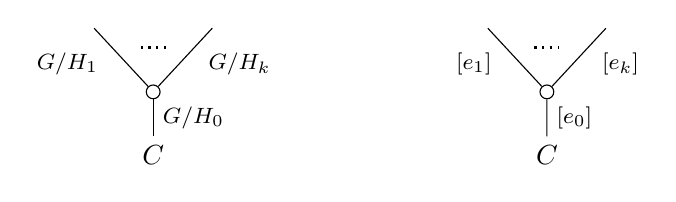
\begin{tikzpicture}
[grow=up,auto,level distance=2.3em,every node/.style = {font=\footnotesize},dummy/.style={circle,draw,inner sep=0pt,minimum size=1.75mm}]
	\node at (0,0) [font=\normalsize]{$C$}
		child{node [dummy] {}
			child{
			edge from parent node [swap,near end] {$G/H_k$} node [name=Kn] {}}
			child{
			edge from parent node [near end] {$G/H_1$}
node [name=Kone,swap] {}}
		edge from parent node [swap] {$G/H_0$}
		};
		\draw [dotted,thick] (Kone) -- (Kn) ;
	\node at (5,0) [font=\normalsize]{$C$}
		child{node [dummy] {}
			child{
			edge from parent node [swap,near end] {$[e_k]$} node [name=Kn] {}}
			child{
			edge from parent node [near end] {$[e_1]$}
node [name=Kone,swap] {}}
		edge from parent node [swap] {$[e_0]$}
		};
		\draw [dotted,thick] (Kone) -- (Kn) ;
\end{tikzpicture}
\]
We will then abbreviate $\sigma^i C = \sigma^{[e_i]} C$, and write $e_i$, $e_i'$ for the two edges of $\sigma^i C $ that degenerate the edge $e_i$ of $C$,
with $e_i$ denoting the inner edge and $e'_i$ the outer
edge.
\[
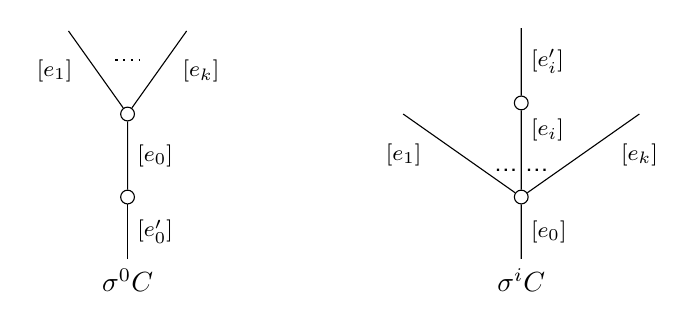
\begin{tikzpicture}
[grow=up,auto,level distance=3em,
every node/.style = {font=\footnotesize},
dummy/.style={circle,draw,inner sep=0pt,minimum size=1.75mm}]
	\node at (0,0) [font=\normalsize]{$\sigma^0 C$}
		child{node [dummy] {}
			child{node [dummy] {}
				child{
				edge from parent node [swap,near end] {$[e_k]$} node [name=Kn] {}}
				child{
				edge from parent node [near end] {$[e_1]$}
node [name=Kone,swap] {}}
			edge from parent node [swap] {$[e_0]$}}
		edge from parent node [swap] {$[e'_0]$}
		};
		\draw [dotted,thick] (Kone) -- (Kn) ;
	\node at (5,0) [font=\normalsize]{$\sigma^i C$}
		child{node [dummy] {}
			child{
			edge from parent node [swap,near end] {$[e_k]$} node [near start,inner sep=1pt,name=Kn] {}}
			child[level distance=3.4em]{node [dummy] {}
				child[level distance=2.7em]{
				edge from parent node [swap] {$[e'_i]$}
}
			edge from parent node [near end,swap] {$[e_i]$}
node [near start,inner sep=1pt,name=Kone,swap] {}
node [near start,inner sep=1pt,name=Kone1] {}}
			child{
			edge from parent node [near end] {$[e_1]$}
node [swap] {}
node [near start,inner sep=1pt,name=Kn1,swap]{}}
		edge from parent node [swap] {$[e_0]$}
		};
		\draw [dotted,thick] (Kone) -- (Kn) ;
		\draw [dotted,thick] (Kone1) -- (Kn1) ;
\end{tikzpicture}
\]
The $G$-tree $\sigma^i C$ then has an orbital inner face\footnote{See \cite[Defn. 2.16]{BP_edss} for a discussion of \textit{orbital} inner faces.}
$\sigma^i C - [e_i]$ obtained by removing $[e_i]$
as well as an orbital outer face obtained by removing $e'_i$,
which we denote $\sigma^i C - [e'_i]$.
Moreover, note that we have natural identifications
$C \simeq \sigma^i C - [e_i]$,
$C \simeq \sigma^i C - [e'_i]$.


In what follows, we will find it convenient to simplify notation by denoting maps $\upsilon_{G,\**}\Omega[T] \to X$,
where $T \in \Omega_G$ and $X \in \mathsf{dSet}_G$,
simply as $T \to X$.


\begin{definition}\label{HOEQUIVS DEF}
	Let $X \in \mathsf{dSet}_G$ be a genuine $G$-$\infty$-operad and $C$ a $G$-corolla with edge orbits
	$[e_0],\cdots,[e_k]$.
%	
	Given two parallel operations 
	$f,g\colon C \rightrightarrows X$,
	we write $f \sim_i g$ if there exists a map
	$H \colon \sigma^i C \to X$ such that
\begin{itemize}
\item $f$ equals the restriction $H|_{\sigma^i C-[e'_i]}$;
\item $g$ equals the restriction $H|_{\sigma^i C-[e_i]}$;
\item the restriction $H|_{\sigma^i [e_i]}$
is the degeneracy $\sigma^i [e_i] \to [e_i] \to C \to X$.
\end{itemize}
\end{definition}


\begin{remark}\label{HOMOTBOUND REM}
	Note that if $f \sim_i g$ then it must be
	$f|_{\partial C} = g|_{\partial C}$.
\end{remark}



\begin{example}\label{EQUIVSIM EX}
	Let $G = \mathbb{Z}_{/2} = \{\pm 1\}$
	and consider the $G$-corolla with orbital and expanded representations as given on the left below.
\[
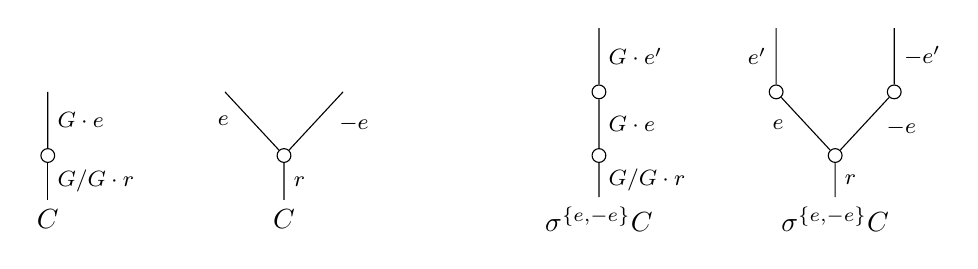
\begin{tikzpicture}
[grow=up,auto,level distance=2.3em,every node/.style = {font=\footnotesize},dummy/.style={circle,draw,inner sep=0pt,minimum size=1.75mm}]
	\node at (0,0) [font=\normalsize]{$C$}
		child{node [dummy] {}
			child{
			edge from parent node [swap] {$G \cdot e$}
node [name=Kone,swap] {}}
		edge from parent node [swap] {$G/G \cdot r$}
		};
	\node at (3,0) [font=\normalsize]{$C$}
		child{node [dummy] {}
			child{
			edge from parent node [swap,near end] {$-e$} node [name=Kn] {}}
			child{
			edge from parent node [near end] {$e$}
node [name=Kone,swap] {}}
		edge from parent node [swap] {$r$}
		};
	\node at (7,0) [font=\normalsize]{$\sigma^{\{e,-e\}} C$}
		child{node [dummy] {}
			child{node [dummy] {}
				child{
				edge from parent node [swap] {$G \cdot e'$}
node [swap] {}}
			edge from parent node [swap] {$G \cdot e$}
node [swap] {}}
		edge from parent node [swap] {$G/G \cdot r$}
		};
	\node at (10,0) [font=\normalsize]{$\sigma^{\{e,-e\}} C$}
		child{node [dummy] {}
			child{node [dummy] {}
				child{
				edge from parent node [swap] {$-e'$} node {}}
			edge from parent node [swap,near end] {$-e$} node {}}
			child{node [dummy] {}
				child{
				edge from parent node {$e'$}
node [swap] {}}
			edge from parent node [near end] {$e$}
node [swap] {}}
		edge from parent node [swap] {$r$}
		};
\end{tikzpicture}
\]
$C$ then has a single leaf $G$-edge orbit $[e] = G \cdot e$, so that for
$f,g \colon C \to X$ it is
$f \sim_1 g$
if there exists a dendrex
$H \colon \sigma^{\{e,-e\}}C \to X$
such that 
\begin{equation}\label{EQUIVHOMOT EQ}
	f = H|_{\sigma^{\{e,-e\}}C - \{e',-e'\}}
\qquad
	g = H|_{\sigma^{\{e,-e\}}C - \{e,-e\}}
\qquad
	H_{\sigma^e e}, H|_{\sigma^{-e}-e} \text{ are degenerate}.
\end{equation}
It is worthwhile to compare this equivariant relation with the relations obtained if one forgets the $G$-actions. Indeed, while \eqref{EQUIVHOMOT EQ} implicitly assumes that all of $f,g,H$ are $G$-equivariant,
by omitting that assumption one can reinterpret 
\eqref{EQUIVHOMOT EQ}
as defining a relation
$f \sim_{[e]} g$ between not necessarily $G$-equivariant maps $f,g \colon C \to X$.

A priori, the $\sim_{[e]}$ relation differs from the 
non-equivariant 
$\sim_{e}$ and $\sim_{-e}$
relations obtained by regarding $C$ as a non-equivariant corolla.
However, for $f,g,H$ as in \eqref{EQUIVHOMOT EQ} one has
\begin{equation}\label{EQUIVSIM EQ}
f = H|_{\sigma^{\{e,-e\}}C - \{e',-e'\}}
\sim_e H|_{\sigma^{\{e,-e\}}C - \{e,-e'\}}
\sim_{-e} H|_{\sigma^{\{e,-e\}}C - \{e,-e\}} =g
\end{equation}
so that, by Lemma \ref{EQUIVI LEM}(b) below one has that
$f \sim_{[e]} g$ in fact implies
$f \sim_{e} g$. Moreover, the converse statement follows immediately by using degeneracies.

More generally, similar considerations show that the $\sim$ relations are compatible with restricting the $G$-actions.
\end{example}



\begin{lemma}[{cf. \cite[Prop. 6.3 and Lemma 6.4]{MW09}}]
	\label{EQUIVI LEM}
	Let $X \in \mathsf{dSet}_G$ be a genuine $G$-$\infty$-operad and $C$ a $G$-corolla with edge orbits
	$[e_0],\cdots,[e_k]$. Then:
\begin{itemize}
	\item[(a)] each of the relations $\sim_i$ 
	in Definition \ref{HOEQUIVS DEF}
	is an equivalence relation;
	\item[(b)] all the equivalence relations $\sim_i$ coincide.
\end{itemize}
\end{lemma}

\begin{proof}
	We first address (a). 
	
	For reflexivity $f \sim_i f$,
	we take the exhibiting homotopy 
	$H$ to be the degeneracy
	$\sigma^i C \xrightarrow{\sigma^i} C \xrightarrow{f} X$.
	
	Both symmetry and transitivity will use the 
	tree $\sigma^{ii} C$ below, which degenerates $[e_i]$ twice.
\[
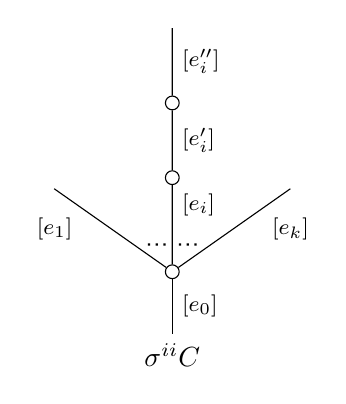
\begin{tikzpicture}
[grow=up,auto,level distance=3em,
every node/.style = {font=\footnotesize},
dummy/.style={circle,draw,inner sep=0pt,minimum size=1.75mm}]
	\node at (0,0) [font=\normalsize]{$\sigma^{ii} C$}
		child{node [dummy] {}
			child{
			edge from parent node [swap,near end] {$[e_k]$} node [near start,inner sep=1pt,name=Kn] {}}
			child[level distance=3.4em]{node [dummy] {}
				child[level distance=2.7em]{node [dummy] {}
					child[level distance=2.7em]{
					edge from parent node [swap] {$[e''_i]$}
}
				edge from parent node [swap] {$[e'_i]$}
}
			edge from parent node [near end,swap] {$[e_i]$}
node [near start,inner sep=1pt,name=Kone,swap] {}
node [near start,inner sep=1pt,name=Kone1] {}}
			child{
			edge from parent node [near end] {$[e_1]$}
node [swap] {}
node [near start,inner sep=1pt,name=Kn1,swap]{}}
		edge from parent node [swap] {$[e_0]$}
		};
		\draw [dotted,thick] (Kone) -- (Kn) ;
		\draw [dotted,thick] (Kone1) -- (Kn1) ;
\end{tikzpicture}
\]
For symmetry, suppose $f \sim_i g$ with 
$H \colon \sigma^{i} C \to X$ the exhibiting homotopy.
Define a map 
$\bar{H} \colon \Lambda^{[e_i]}_o[\sigma^{ii} C] \to X$ by
\[
	\bar{H}|_{\sigma^{ii}C - [e''_i]} = H,
		\qquad
	\bar{H}|_{\sigma^{ii}C - [e'_i]} = f \circ \sigma^i,
		\qquad
	\bar{H}|_{\sigma^{ii} [e_i]} = 
	f|_{[e_i]} \circ \sigma^{ii} =
	g|_{[e_i]} \circ \sigma^{ii}.
\]
Since the orbital inner horn inclusion
$\bar{H} \colon \Lambda^{[e_i]}_o[\sigma^{ii} C] \to \Omega[C]$
is $G$-inner anodyne by \cite[Prop. 3.13]{BP_edss},
$\bar{H}$ admits an extension $\widetilde{H} \colon \sigma^{ii}C \to X$.
The restriction $\widetilde{H}|_{\sigma^{ii}C - [e_i]}$ then provides the homotopy exhibiting $g \sim_i f$, and symmetry of $\sim_i$ follows.

Next, suppose $f \sim_i g$ and $g \sim_i h$, and let 
$H \colon \sigma^{i} C \to X$,
$K \colon \sigma^{i} C \to X$ be the exhibiting homotopies.
Define a map 
$\bar{H} \colon \Lambda^{[e'_i]}_o[\sigma^{ii} C] \to X$ by
\[
	\bar{H}|_{\sigma^{ii}C - [e''_i]} = H,
		\qquad
	\bar{H}|_{\sigma^{ii}C - [e_i]} = K,
		\qquad
	\bar{H}|_{\sigma^{ii} [e_i]} = 
	f|_{[e_i]} \circ \sigma^{ii} =
	g|_{[e_i]} \circ \sigma^{ii} =
	h|_{[e_i]} \circ \sigma^{ii}.
\]
$\bar{H}$ again admits an extension $\widetilde{H} \colon \sigma^{ii}C \to X$, 
and the restriction $\widetilde{H}|_{\sigma^{ii}C - [e'_i]}$
provides the homotopy exhibiting $f \sim_i g$, and transitivity of $\sim_i$ follows.


We next turn to (b). Consider the tree $\sigma^{ij} C$ which degenerates $C$ once along each of $[e_i]$ and $[e_j]$.
\[
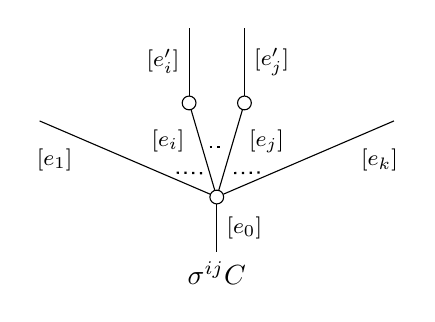
\begin{tikzpicture}
[grow=up,auto,level distance=2.75em,
every node/.style = {font=\footnotesize},
dummy/.style={circle,draw,inner sep=0pt,minimum size=1.75mm}]
	\node at (0,0) [font=\normalsize]{$\sigma^{ij} C$}
		child{node [dummy] {}
			child{
			edge from parent node [swap,near end] {$[e_k]$} node [near start,inner sep=1pt,name=Kn] {}}
			child[level distance=3.4em,sibling distance=2em]{node [dummy] {}
				child[level distance=2.7em]{
				edge from parent node [swap] {$[e'_j]$}
}
			edge from parent node [very near end,swap] {$[e_j]$}
node [near start,inner sep=1pt,name=Kone,swap] {}
node [inner sep=1pt,name=Kn2] {}}
			child[level distance=3.4em,sibling distance=2em]{node [dummy] {}
				child[level distance=2.7em]{
				edge from parent node {$[e'_i]$}
}
			edge from parent node [very near end] {$[e_i]$}
node [inner sep=1pt,name=Kone2,swap] {}
node [near start,inner sep=1pt,name=Kone1] {}}
			child{
			edge from parent node [near end] {$[e_1]$}
node [swap] {}
node [near start,inner sep=1pt,name=Kn1,swap]{}}
		edge from parent node [swap] {$[e_0]$}
		};
		\draw [dotted,thick] (Kn) -- (Kone) ;
		\draw [dotted,thick] (Kone1) -- (Kn1) ;
		\draw [dotted,thick] (Kone2) -- (Kn2) ;
\end{tikzpicture}
\]
Suppose $f \sim_i g$ with $H \colon \sigma^{i} C \to X$ the associated homotopy.
Define a map 
$\bar{H} \colon \Lambda^{[e_i]}_o[\sigma^{ij} C] \to X$ by
\[
	\bar{H}|_{\sigma^{ij}C - [e'_j]} = H,
		\qquad
	\bar{H}|_{\sigma^{ij}C - [e_j]} = f \circ \sigma^i,
		\qquad
	\bar{H}|_{\sigma^{ij}C - [e'_i]} = f \circ \sigma^j.
\]
Yet again, $\bar{H}$ admits an extension $\widetilde{H} \colon \sigma^{ij}C \to X$, and the restriction $\widetilde{H}|_{\sigma^{ij}C - [e_i]}$
provides a homotopy exhibiting $g \sim_j f$. (b) now follows.
\end{proof}



In light of Lemma \ref{EQUIVI LEM},
given parallel operations $f,g \colon C \rightrightarrows X$ with 
$C$ a $G$-corolla and $X$ a genuine $G$-$\infty$-operad,
we will henceforth write $f \sim g$ whenever $f \sim_i g$ for some (and thus all) $i$.
We now extend the $\sim$ relation.

\begin{definition}\label{XTENDSIM DEF}
	Let $T \in \Omega_G$ be a $G$-tree
	and $X \in \mathsf{dSet}_G$ be a 
	genuine $G$-$\infty$-operad.
	
	Given dendrices $x,y\colon T \to X$ we write
	$x \sim y$ if there are equivalences of restrictions
	$x|_{T_v} \sim y|_{T_v}$ for all $G$-vertices
	$v \in \boldsymbol{V}_G(T)$.
	
	Further, we define $\tau_G(X)(T) = X(T)/\sim$.
\end{definition}



\begin{proposition}
	Let $X \in \mathsf{dSet}_G$ be a genuine $G$-$\infty$-operad. Then the assignment 
	$T \mapsto \tau_G(X)(T)$
	is a contravariant functor in $T \in \Omega_G$, i.e.
	$\tau_G(X) \in \mathsf{dSet}_G$.
\end{proposition}

\begin{proof}
	It suffices to show that the $\sim$ equivalence relations are compatible with the generating classes of maps in $\Omega_G$, namely
	degeneracies, inner faces, outer faces, and quotient maps.
	
	The cases of degeneracies and outer faces are obvious. In the case of quotients, 
	since any quotient $\bar{T} \to T$ of $G$-trees induces quotients on $G$-vertices, it suffices to consider the case of a quotient
	$\bar{C} \xrightarrow{\pi} C$ of $G$-corollas.
	But it is then straightforward to check that if a homotopy exhibiting $f \sim_0 g$ also induces a homotopy exhibiting 
	$f \circ \pi \sim_0 g \circ \pi$
	(notably, the same needs not be true for the relations $f \sim_i g$ when $0<i$, 
	in which case the exhibiting homotopy 
	may instead exhibit a string of relations 
	$f \circ \pi \sim \cdots \sim g \circ \pi$
	as in \eqref{EQUIVSIM EQ}).

It remains to address the most interesting case,
that of inner faces. Since inner faces can be factored as composites of inner faces that collapse a singe inner edge orbit,
it suffices to consider the case of faces
$D \to T$ where $T$ has a single inner edge orbit; that is,
we can assume that there are $G$-corollas
$C_1$, $C_2$ such that 
$T = C_1 \amalg_{[e_i]} C_2$ and
$D = T - [e_i]$, as illustrated below.
\[
\begin{tikzpicture}
[grow=up,auto,level distance=3em,
every node/.style = {font=\footnotesize},
dummy/.style={circle,draw,inner sep=0pt,minimum size=1.75mm}]
	\node at (0,0) [font=\normalsize]{$C_1$}
		child{node [dummy] {}
			child[level distance=2.15em]{
			edge from parent node [swap,near end] {} node [inner sep=1pt,name=Kn] {}}
			child[level distance=4.5em]{node {}
			edge from parent node [pos=0.65,swap] {$[e_i]$}
node [near start,inner sep=1pt,name=Kone,swap] {}
node [near start,inner sep=1pt,name=Kone1] {}}
			child[level distance=2.15em]{
			edge from parent node [near end] {}
node [swap] {}
node [inner sep=1pt,name=Kn1,swap]{}}
		edge from parent node [swap] {$[e_0]$}
		};
		\draw [dotted,thick] (Kone) -- (Kn) ;
		\draw [dotted,thick] (Kone1) -- (Kn1) ;
	\node at (4,0) [font=\normalsize]{$C_2$}
		child{node [dummy] {}
			child{
			edge from parent node [swap,near end] {} node [name=Kn] {}}
			child{
			edge from parent node [near end] {}
node [name=Kone,swap] {}}
		edge from parent node [swap] {$[e_i]$}
		};
		\draw [dotted,thick] (Kone) -- (Kn) ;
	\node at (9,0) [font=\normalsize]{$T$}
		child{node [dummy] {}
			child[level distance=2.15em]{
			edge from parent node [swap,near end] {} node [inner sep=1pt,name=Kn] {}}
			child[level distance=4.5em]{node [dummy] {}
				child[level distance=3em]{
				edge from parent node [swap,near end] {} node [name=Kn2] {}}
				child[level distance=3em]{
				edge from parent node [near end] {}
node [name=Kone2,swap] {}}
			edge from parent node [pos=0.65,swap] {$[e_i]$}
node [near start,inner sep=1pt,name=Kone,swap] {}
node [near start,inner sep=1pt,name=Kone1] {}}
			child[level distance=2.15em]{
			edge from parent node [near end] {}
node [swap] {}
node [inner sep=1pt,name=Kn1,swap]{}}
		edge from parent node [swap] {$[e_0]$}
		};
		\draw [dotted,thick] (Kone) -- (Kn) ;
		\draw [dotted,thick] (Kone1) -- (Kn1) ;
		\draw [dotted,thick] (Kone2) -- (Kn2) ;
\end{tikzpicture}
\]
The claim is now that if
$x,y \colon T \to X$ are such that
$x|_{C_1} \sim y|_{C_1}$ and
$x|_{C_2} \sim y|_{C_2}$
then it is also 
$x|_{D} \sim y|_{D}$.
This will follow from the following two claims:
\begin{itemize}
\item[(i)] if $x,y \colon T \to X$ are such that
$x|_{C_1} = y|_{C_1}$ and
$x|_{C_2} = y|_{C_2}$
then $x|_{D} \sim y|_{D}$;
\item[(ii)]
given $x \colon T \to X$, $f\colon C_1 \to X$ and
$g \colon C_2 \to X$ such that
$f \sim x|_{C_1}$, $g \sim x|_{C_2}$,
there exists
$y \colon T \to X$ such that
$y|_{C_1} = f$, $y|_{C_2} = g$ and
$y|_D = x|_D$.
\end{itemize}
To show (i) and (ii), consider the degeneracies
$\sigma^0 T$ and $\sigma^i T$ pictured below.
\[
\begin{tikzpicture}
[grow=up,auto,level distance=3em,
every node/.style = {font=\footnotesize},
dummy/.style={circle,draw,inner sep=0pt,minimum size=1.75mm}]
	\node at (0,0) [font=\normalsize]{$\sigma^0 T$}
		child{node [dummy] {}
		child{node [dummy] {}
			child{
			edge from parent node [swap,near end] {} node [near start,inner sep=1pt,name=Kn] {}}
			child[level distance=3.4em]{node [dummy] {}
				child{
				edge from parent node [swap,near end] {} node [name=Kn2] {}}
				child{
				edge from parent node [near end] {}
node [name=Kone2,swap] {}}
			edge from parent node [near end,swap] {$[e_i]$}
node [near start,inner sep=1pt,name=Kone,swap] {}
node [near start,inner sep=1pt,name=Kone1] {}}
			child{
			edge from parent node [near end] {}
node [swap] {}
node [near start,inner sep=1pt,name=Kn1,swap]{}}
		edge from parent node [swap] {$[e_0]$}}
		edge from parent node [swap] {$[e'_0]$}
		};
		\draw [dotted,thick] (Kone) -- (Kn) ;
		\draw [dotted,thick] (Kone1) -- (Kn1) ;
		\draw [dotted,thick] (Kone2) -- (Kn2) ;
	\node at (6,0) [font=\normalsize]{$\sigma^i T$}
		child{node [dummy] {}
			child{
			edge from parent node [swap,near end] {} node [near start,inner sep=1pt,name=Kn] {}}
			child[level distance=3.4em]{node [dummy] {}
			child{node [dummy] {}
				child{
				edge from parent node [swap,near end] {} node [name=Kn2] {}}
				child{
				edge from parent node [near end] {}
node [name=Kone2,swap] {}}
			edge from parent node [swap] {$[e'_i]$}}
			edge from parent node [near end,swap] {$[e_i]$}
node [near start,inner sep=1pt,name=Kone,swap] {}
node [near start,inner sep=1pt,name=Kone1] {}}
			child{
			edge from parent node [near end] {}
node [swap] {}
node [near start,inner sep=1pt,name=Kn1,swap]{}}
		edge from parent node [swap] {$[e_0]$}
		};
		\draw [dotted,thick] (Kone) -- (Kn) ;
		\draw [dotted,thick] (Kone1) -- (Kn1) ;
		\draw [dotted,thick] (Kone2) -- (Kn2) ;
\end{tikzpicture}
\]
Given $x,y$ as in (i), one can now build a map
$H \colon \Lambda_o^{[e_i]}[\sigma^0 T] \to X$ by
\[
	H|_{\sigma^0 T - [e_0]} = x,
\qquad
	H|_{\sigma^0 T - [e'_0]} = y,
\qquad
	H|_{\sigma^0 C_1} = 
	x|_{C_1} \circ \sigma^0 = 
	y|_{C_1} \circ \sigma^0.
\]
Letting $\widetilde{H}\colon \sigma^0 T \to X$
be an extension of $H$,
the restriction $H|_{\sigma^0 T - [e_i]}$
provides the desired homotopy 
$x|_{D} \sim y|_{D}$, showing (i).


Lastly, let $x,f,g$ be as in (ii), 
and let
$K \colon \sigma^i C_1 \to X$ exhibit the relation
$f \sim_i x|_{C_1}$
and 
$ \bar{K} \colon \sigma^i C_2 \to X$
exhibit the relation
$x|_{C_2} \sim_i g$ (note the reversed order).
Now build the map
$H \colon \Lambda_o^{[e'_i]}[\sigma^i T] \to X$ by
\[
	H|_{\sigma^i T - [e_i]} = x,
\qquad
	H|_{\sigma^i C_1} = K,
\qquad
	H|_{\sigma^i C_2} = \bar{K}.
\]
Again letting 
$\widetilde{H} \colon \sigma^i T \to X$ be a lift,
the restriction 
$\widetilde{H}|_{\sigma^i T - [e'_i]}$
provides the desired $y \colon T \to X$ in (ii),
finishing the proof.
\end{proof}


\begin{corollary}\label{HOOPUNIV COR}
Let $X \in \mathsf{dSet}_G$ be a genuine $G$-$\infty$-operad. Then
	\begin{itemize}
	\item[(a)] $\tau(X) \in \mathsf{dSet}_G$ is a genuine equivariant operad, i.e. it satisfies the strict right lifting condition against the Segal core inclusions
	$Sc[T] \to \Omega[T]$ for $T \in \Omega_G$;
	\item[(b)] the quotient map
	$\upsilon_{\**}X \to \tau_G(X)$ is the universal map from $\upsilon_{\**}X$ to a genuine equivariant operad.
	\end{itemize}
\end{corollary}

\begin{proof}
	Note first that by Remark \ref{HOMOTBOUND REM}
	any map $Sc[T] \to \tau_G(X)$ admits a factorization 
	$Sc[T] \to X \xrightarrow{q} \tau_G(X)$.
	
	The right lifting property for $\tau_G(X)$
	against the maps $Sc[T] \to \Omega[T]$
	is then automatic from the lifting property for $X$.

	For strictness,	
	note that Definition \ref{XTENDSIM DEF}
	can be reinterpreted as saying that
	a pair of dendrices $\Omega[T] \rightrightarrows X$
	give rise to the same point of 
	$\tau_G(X)$, i.e. 
	the composites 
	$\Omega[T] \rightrightarrows X \xrightarrow{q}
	\tau_G(X)$ coincide, 
	iff the composites 
	$Sc[T] \to \Omega[T] \rightrightarrows X \xrightarrow{q}
	\tau_G(X)$ coincide, showing strictness, and thus (a).
		
	For (b), since $\tau_G(X)$ is a quotient of
	$X$, it suffices to show that any map
	of the form $F \colon X \to Y$ with $Y$ a genuine equivariant operad must also enforce the $\sim$ relation.
	For a $G$-corolla $C$ and
	$f,g\colon C \rightrightarrows X$ such that 
	$H \colon \sigma^i C \to X$ exhibits
	$f \sim_i g$, 
	the strict lifting condition for $Y$
	shows that the maps
	$F\circ H \colon \sigma^i C \to Y$,
	$F(f) \circ \sigma^i \colon \sigma^i C \to Y$
	must coincide, and thus that
	$F(f)=F(g)$.
	The further claim that $F$ respects equivalences
	of general pairs of dendrices $T \rightrightarrows X$
	is immediate from Definition \ref{XTENDSIM DEF}.
\end{proof}




The following is the analogue of \cite[Prop. 4.8]{CM13b}.

\begin{proposition}\label{HOOPID_PROP}
Let $\mathcal{O} \in \mathsf{sOp}^G$
be a fibrant operad. 
Then there is a natural isomorphism of genuine equivariant operads
\begin{equation}\label{HOOPID EQ}
\tau_G(hcN(\mathcal{O})) \xrightarrow{\simeq}
\pi_0 \left( \upsilon_{\**} N\mathcal{O} \right).
\end{equation}
\end{proposition}


\begin{proof}
      By \cite[Prop. 5.9]{BP_edss}, $\pi_0(\upsilon_{\**}N\O)$ is a genuine equivariant operad,
      and the existence of the map in \eqref{HOOPID EQ}
      will be an application of
      Corollary \ref{HOOPUNIV COR}(b).

Firstly,
note that we have the following identifications,
naturally in $T \in \Omega_G$.
\[
\upsilon_{\**}hcN(\O)(T)
\simeq
\mathsf{sOp}^G(W_!\Omega[T],\O)
\simeq
\mathsf{sdSet}^G(N W_!\Omega[T],N \O)
\simeq 
\mathsf{sdSet}_G(\upsilon_{\**}N W_!\Omega[T],\upsilon_{\**}N \O)
\]
where the second and third identifications use the fact that 
$N\colon \mathsf{Op} \to \mathsf{dSet}$ and $\upsilon_{\**} \colon \dSet^G \to \dSet_G$
are fully faithful inclusions. 
One now has a map
\begin{align*}
  \mathsf{sdSet}_G(\upsilon_{\**}N W_!\Omega[T],\upsilon_{\**}N \O)
  & \to
    \mathsf{sdSet}_G(\upsilon_{\**}N W_!\Omega[T],\pi_0\upsilon_{\**}N \O)
  \\ & \simeq
       \mathsf{dSet}_G(\pi_0 \upsilon_{\**}  N W_!\Omega[T],\pi_0\upsilon_{\**}N \O)
  \\ & \simeq
       \mathsf{dSet}_G(\upsilon_{\**}\Omega[T],\pi_0\upsilon_{\**}N \O)
  \\ & =
       (\pi_0\upsilon_{\**}N \O)(T)
\end{align*}
so altogether we obtain a map
$\upsilon_{\**}hcN(\O) \to \pi_0 \upsilon_{\**} N \O$
and hence, by Corollary \ref{HOOPUNIV COR},
the desired map 
\[
	\tau_G(hcN(\O)) \to \pi_0 \upsilon_{\**} N \O
\]
Moreover, both of these are quotients of $\upsilon_{\**}hcN(\O)$,
so to prove that this map is an isomorphism one needs only show that any two parallel operations $C \rightrightarrows hcN \O$ of $\upsilon_{\**}hcN(\O)$
that are identified in 
$\pi_0 \upsilon_{\**} N \O$
were already identified in 
$\tau_G(hcN(\O))$.
But this now follows immediately from the pushout from Proposition \ref{WLEFTQPUSH LEM}
\[
\begin{tikzcd}
	\Omega(C) \otimes_{\mathfrak{C}_{\bullet}}
	\partial \Delta[1]
	\ar{r} \ar{d}
&
	W_! \left(\partial \Omega[\sigma^0 C]\right) 
	\ar{d}
\\
	\Omega(C) \otimes_{\mathfrak{C}_{\bullet}}
	\Delta[1]
	\ar{r}
&
	W(\sigma^0 C)
\end{tikzcd}
\]
\end{proof}










\bibliography{biblio3}{}
\bibliographystyle{amsalpha2}



\end{document}


%%% Local Variables:
%%% mode: latex
%%% TeX-master: t
%%% End:
